% Preamble-ish commands {{{
\newcommand{\sectionbreak}{\clearpage}
\newcommand*{\aqeff}{\mathrm{AQ_{eff}}}
\renewcommand*{\thefigure}{S\arabic{figure}}
\renewcommand*{\thetable}{S\arabic{table}}
\renewcommand*{\thepage}{S\arabic{page}}
\setcounter{page}{1}
\setcounter{figure}{0}
\setcounter{table}{0}
\onehalfspacing
% }}}
% Title page {{{
\hspace{0pt}
\vfill
\begin{center}
    \huge
    Supporting Information

    \textit{for}

    \hsqctitle{}

    \vspace{1cm}

    \Large Jonathan R.\ J.\ Yong,\textsuperscript{1} Alexandar L.\ Hansen,\textsuperscript{2} {\=E}riks Kup{\v{c}}e,\textsuperscript{3} Tim D.\ W.\ Claridge\textsuperscript{1,}*

    \vspace{1cm}

    \large \textsuperscript{1} \textit{Chemistry Research Laboratory, Department of Chemistry, University of Oxford, Mansfield Road, Oxford, OX1 3TA, U.K.}

    \textsuperscript{2} \textit{Campus Chemical Instrument Center, The Ohio State University, 460 W.\ 12th Avenue, Columbus, OH, 43210 U.S.}

    \textsuperscript{3} \textit{Bruker UK Ltd., Banner Lane, Coventry, CV4 9GH, U.K.}

    * \texttt{tim.claridge@chem.ox.ac.uk}
\end{center}
\thispagestyle{empty}
\vfill
\hspace{0pt}
\newpage
%}}}

% Table of contents {{{
\tableofcontents

\newpage
%}}}

\section{Product operator analysis for pulse sequences}

\begin{figure}
    \centering
    % Inkscape
    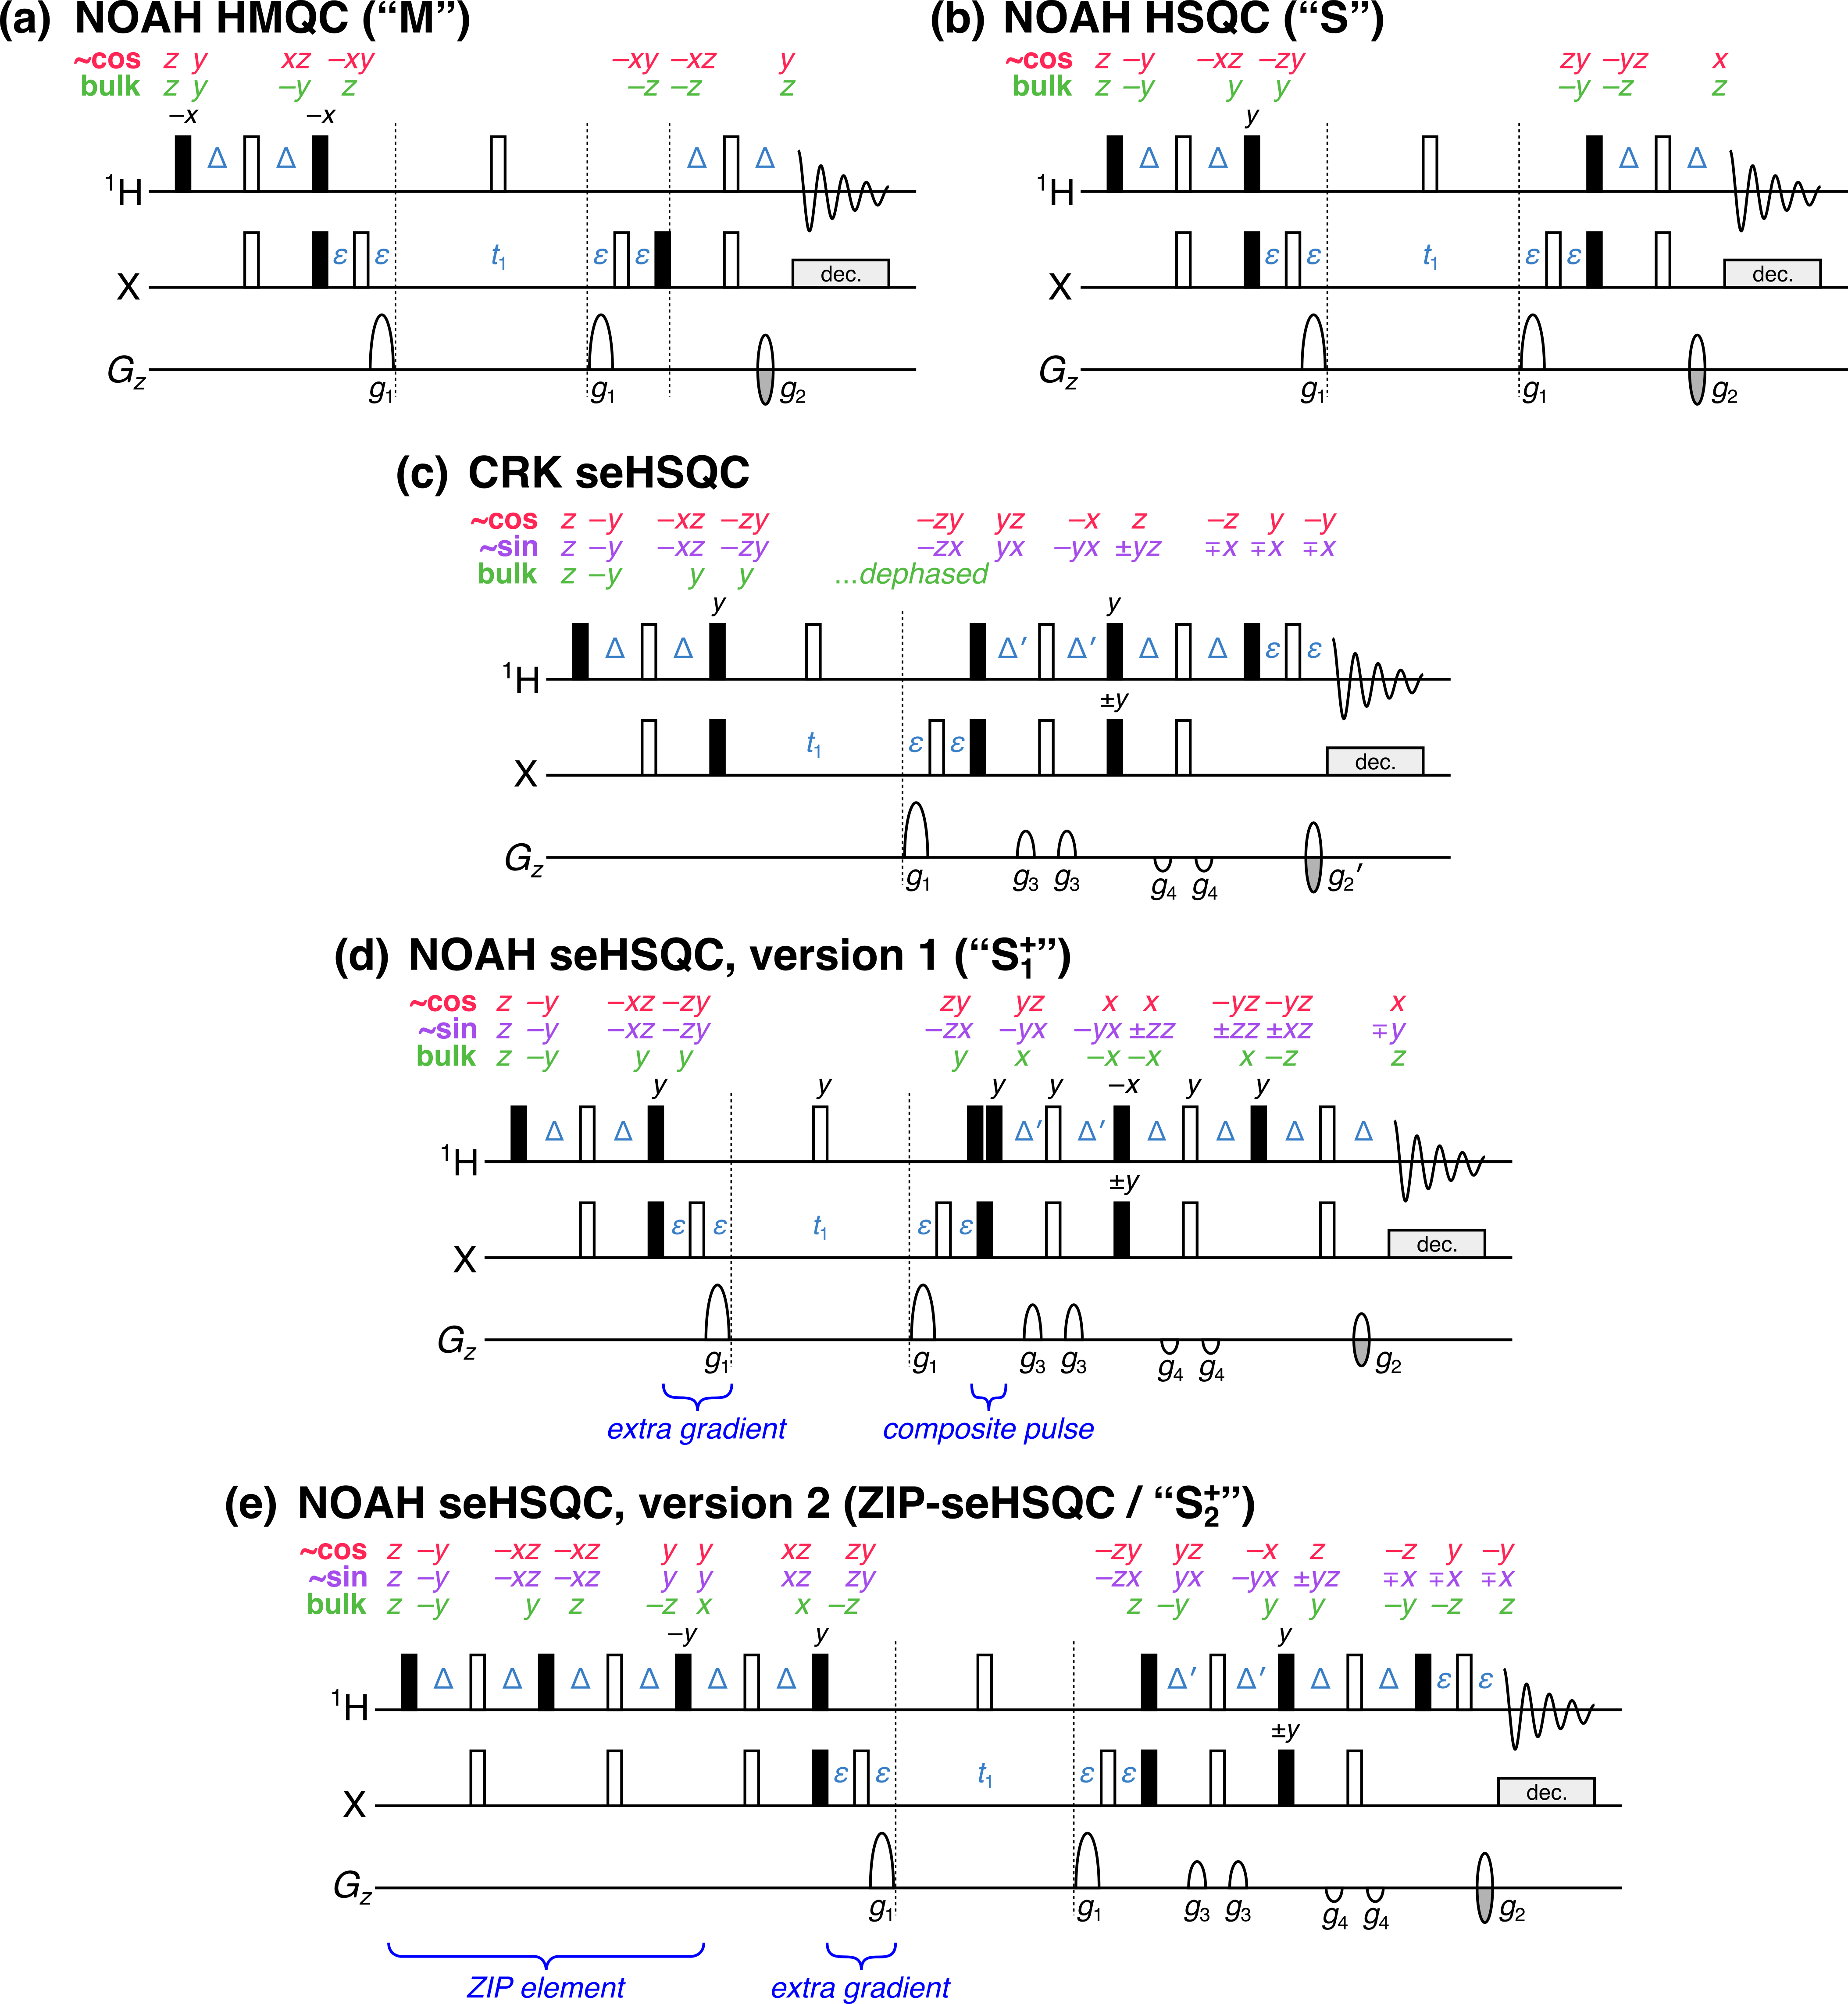
\includegraphics[width=0.82\textwidth]{pprogs_prodop.png}
    {\phantomsubcaption\label{fig:pprogs_prodop_hmqc}}
    {\phantomsubcaption\label{fig:pprogs_prodop_hsqc}}
    {\phantomsubcaption\label{fig:pprogs_prodop_crk}}
    {\phantomsubcaption\label{fig:pprogs_prodop_spv1}}
    {\phantomsubcaption\label{fig:pprogs_prodop_spv2}}
    \caption{
        Product operators for an IS spin system at each stage of the HSQC and seHSQC sequences described in the main text.
        One-letter terms $m$ ($m \in \{x, y, z\}$) are shorthand for single-spin terms on proton, i.e.\ $\hat{I}_m$.
        Two-letter terms $mn$ are shorthand for two-spin terms on both the proton and heteronucleus, i.e.\ $2\hat{I}_m\hat{S}_n$.
        ``$\sim$cos'' represents the pathway for \magn{\ce{C}} magnetisation that is cosine-modulated after $t_1$: for the HMQC and HSQC, this is the only component that is detected.
        For the seHSQC, the sine-modulated \magn{\ce{C}} component (labelled with ``$\sim$sin'') is also detected.
        ``bulk'' refers to the bulk \magnnot{\ce{C}} magnetisation, i.e.\ protons that are not directly coupled to the heteronucleus.
        Note that this analysis assumes $\Delta = \Delta' = 1/(4\cdot\onejxh)$.
        All other symbols have the same meaning as in \cref{fig:pprogs} of the main text.
        \textbf{\subref{fig:pprogs_prodop_hmqc}} NOAH HMQC (``\noahM{}'').
        \textbf{\subref{fig:pprogs_prodop_hsqc}} NOAH HSQC (``\noahS{}'').
        \textbf{\subref{fig:pprogs_prodop_crk}} Cavanagh--Rance--Kay seHSQC; notice that the bulk magnetisation is dephased by the lone $t_1$ gradient.
        \textbf{\subref{fig:pprogs_prodop_spv1}} NOAH seHSQC, version 1 (``\noahSpa{}'').
        \textbf{\subref{fig:pprogs_prodop_spv2}} NOAH seHSQC, version 2 (``\noahSpb{}'').
        Immediately following the ZIP pulse sequence element, directly bonded protons are rotated onto $+y$, whereas the bulk magnetisation is rotated onto $+x$.
    }
    \label{fig:pprogs_prodop}
\end{figure}

\section{Origin and suppression of wing artefacts}

The origin of the ``wing'' artefacts in the final homonuclear modules can be most clearly seen from the following series of experiments involving the NOAH-3 \nitrogen{} seHSQC/\carbon{} ZIP-seHSQC/CLIP-COSY (\noahthree{Spn}{Spb}{Cc}) supersequence.
As described in the main text, if the extra gradient before $t_1$ is not present, each peak in the COSY with an indirect-dimension frequency of $f_1 = \Omega_{\ce{H}}$ is flanked by a pair of artefacts at
\begin{align*}
    f_1 &= \Omega_{\ce{H}} \pm \Omega_{\ce{H}} \cdot \left(\frac{\mathrm{SW_{COSY}}}{2 \cdot \mathrm{SW_{HSQC}}}\right),
\end{align*}

where $\Omega_{\ce{H}}$ is the offset of the relevant proton and $\mathrm{SW}$ refers to the indirect-dimension spectral width.
Since the $f_1$ spectral widths of the two seHSQC modules are different, they lead to distinct sets of wing artefacts in the COSY.
In the spectra shown in the following figures, we have
\begin{align*}
    \mathrm{SW_{\ce{^15N}\,HSQC}} &= \SI{2128}{\Hz} \\
    \mathrm{SW_{\ce{^13C}\,HSQC}} &= \SI{23810}{\Hz} \\
    \mathrm{SW_{COSY}}            &= \SI{8418}{\Hz}
\end{align*}

meaning that the artefacts coming from the \nitrogen{} seHSQC occur at $f_1 = (1.00 \pm 1.98) \Omega_{\ce{H}}$ (and are therefore often folded), whereas artefacts coming from the \carbon{} seHSQC occur at $f_1 = (1.00 \pm 0.18) \Omega_{\ce{H}}$ (and are typically found very close to the main peak).
In both cases, the artefacts associated with intense methyl group peaks are the most obvious, but similar artefacts are observed for all other peaks, albeit with lower absolute intensities.

\begin{figure}
    \centering
    % figures/wing_artefacts.py
    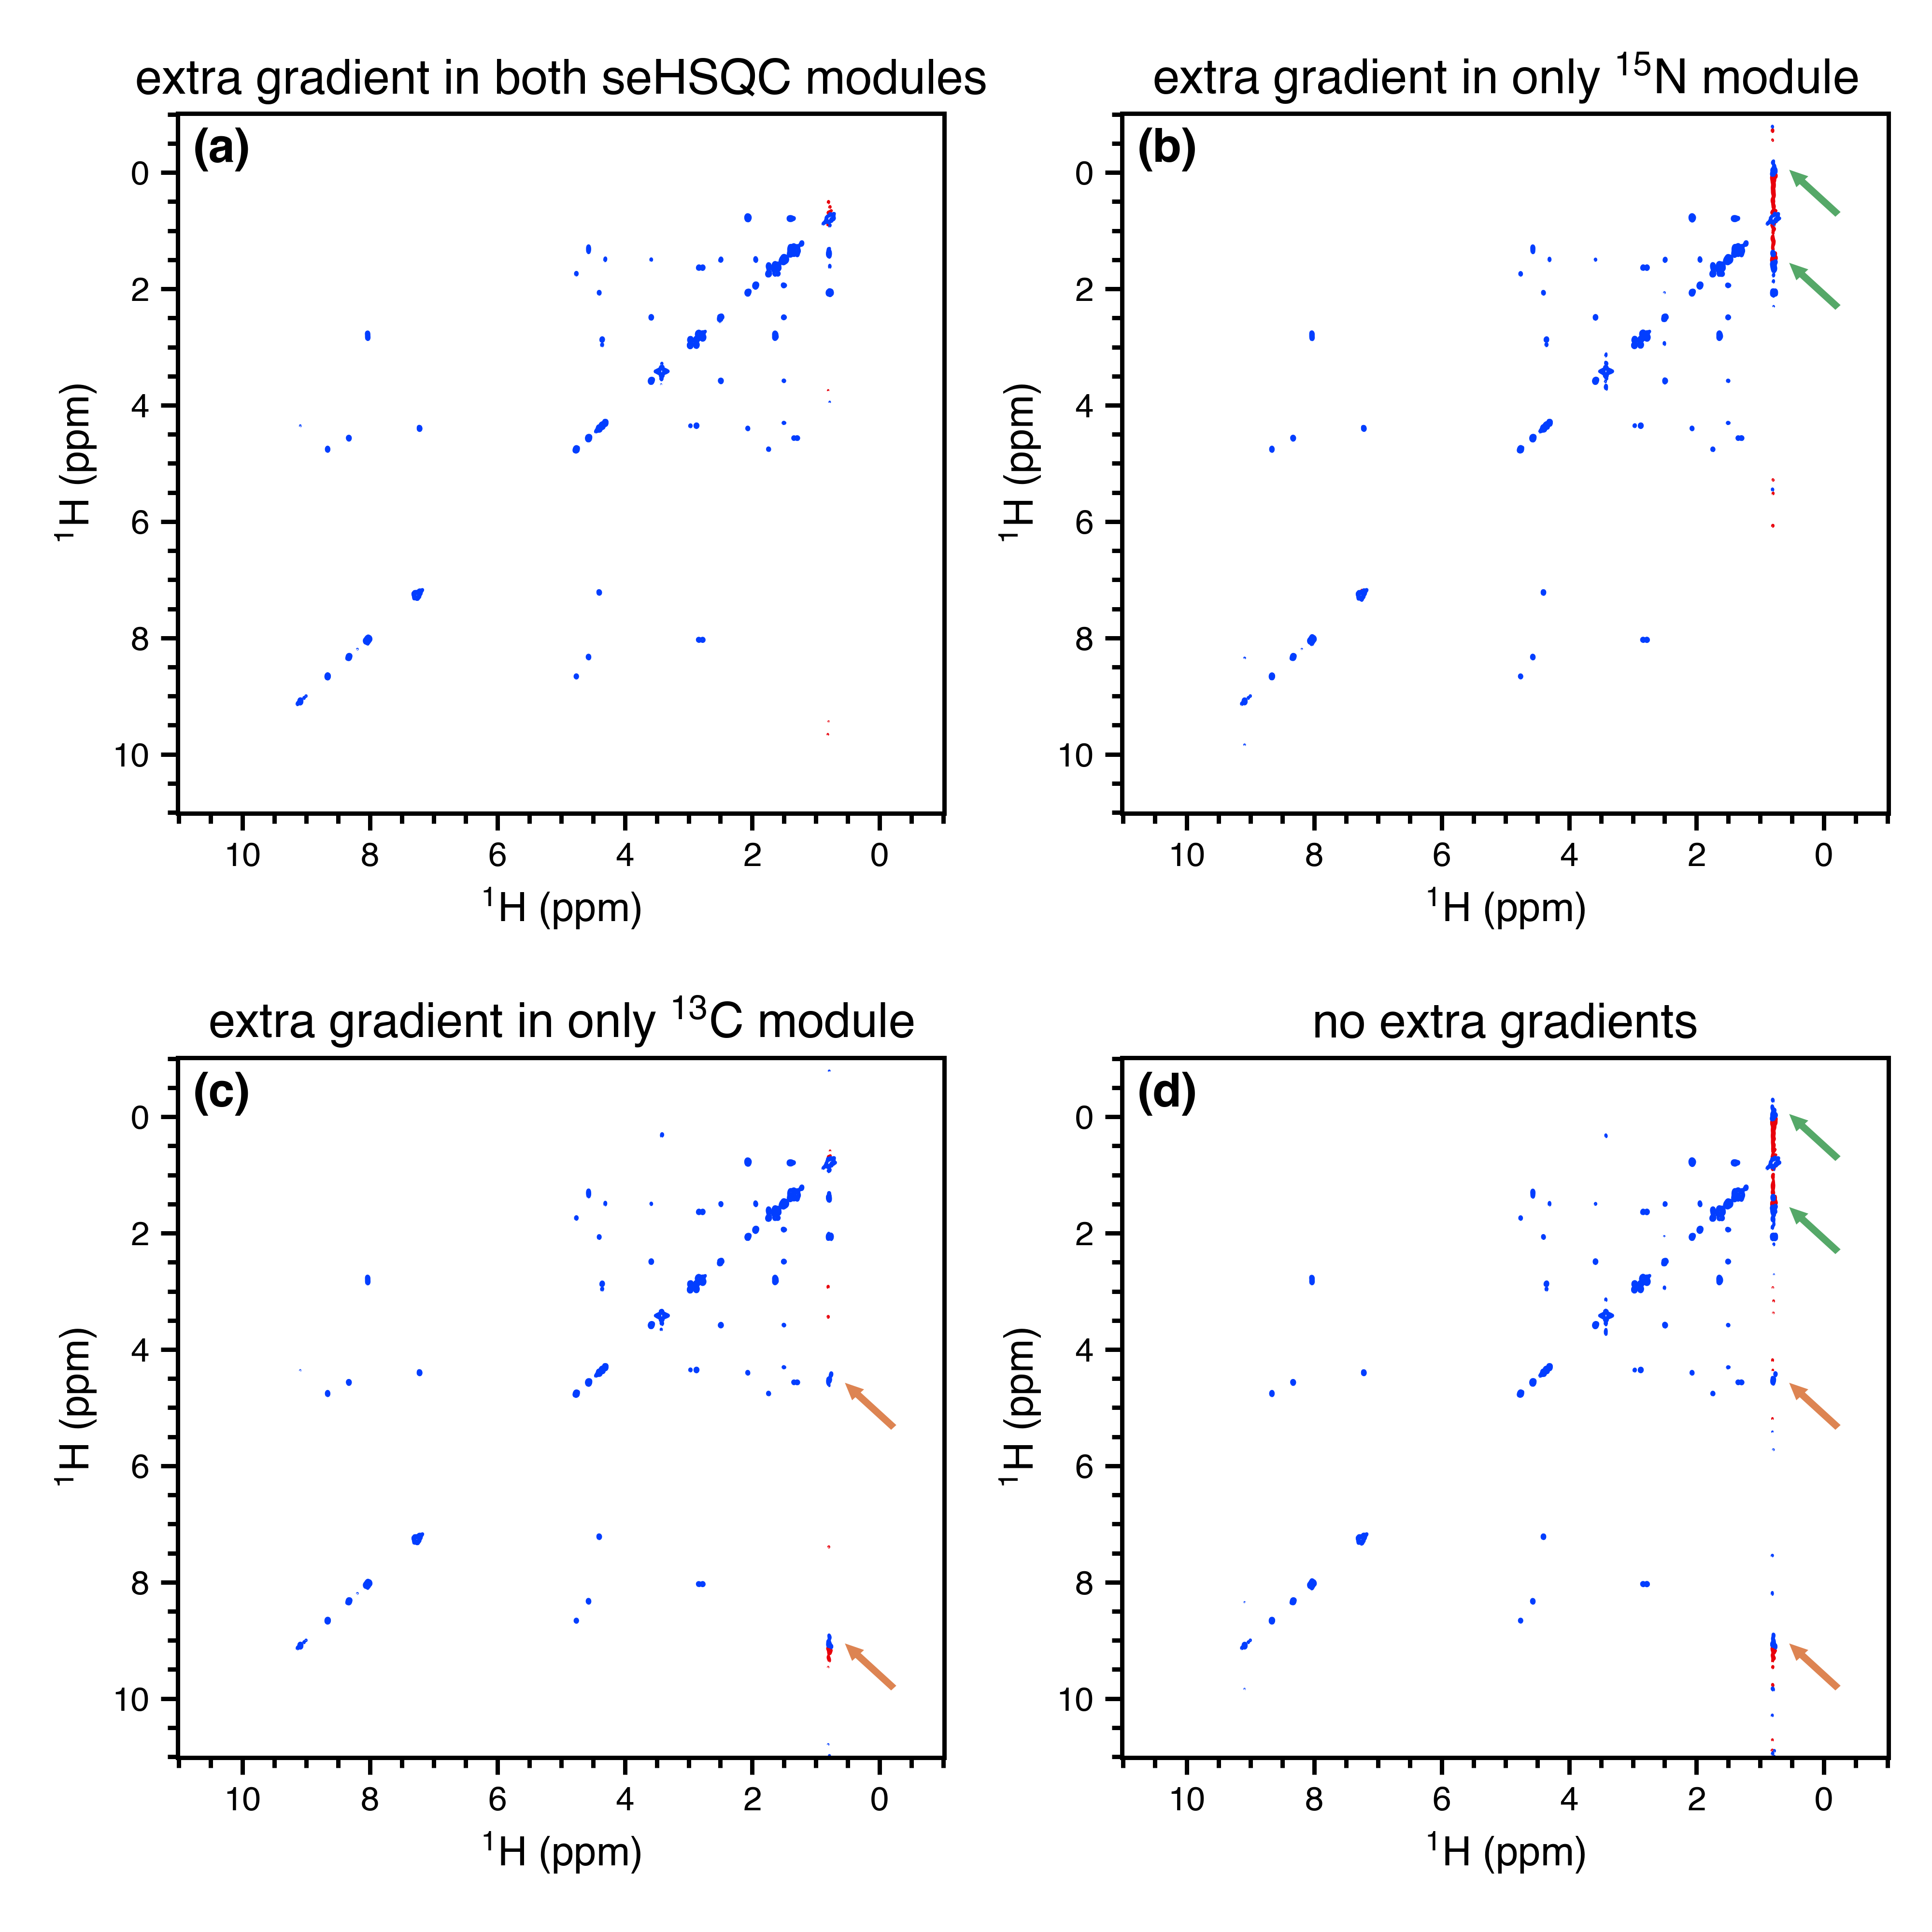
\includegraphics[width=0.8\textwidth]{wing_artefacts.png}
    \caption{
        CLIP-COSY spectra obtained from various forms of the NOAH-3 \noahthree{Spn}{Spb}{Cc} supersequence.
        Wing artefacts arising from the \nitrogen{} seHSQC are highlighted in orange; those arising from the \carbon{} seHSQC in green.
        Notice how (in this case) the former can easily be misinterpreted as a crosspeak, while the latter obscures genuine crosspeaks.
        \textbf{(a)} With the extra gradient inserted for both modules, i.e.\ no artefacts.
        \textbf{(b)} With an extra gradient in only the \nitrogen{} module, i.e.\ only the \carbon{} artefacts.
        \textbf{(c)} With an extra gradient in only the \carbon{} module.
        \textbf{(d)} With no extra gradients.
        \grami{}
    }
    \label{fig:wing_artefacts}
\end{figure}

\begin{figure}
    \centering
    % figures/wing_artefacts2.py
    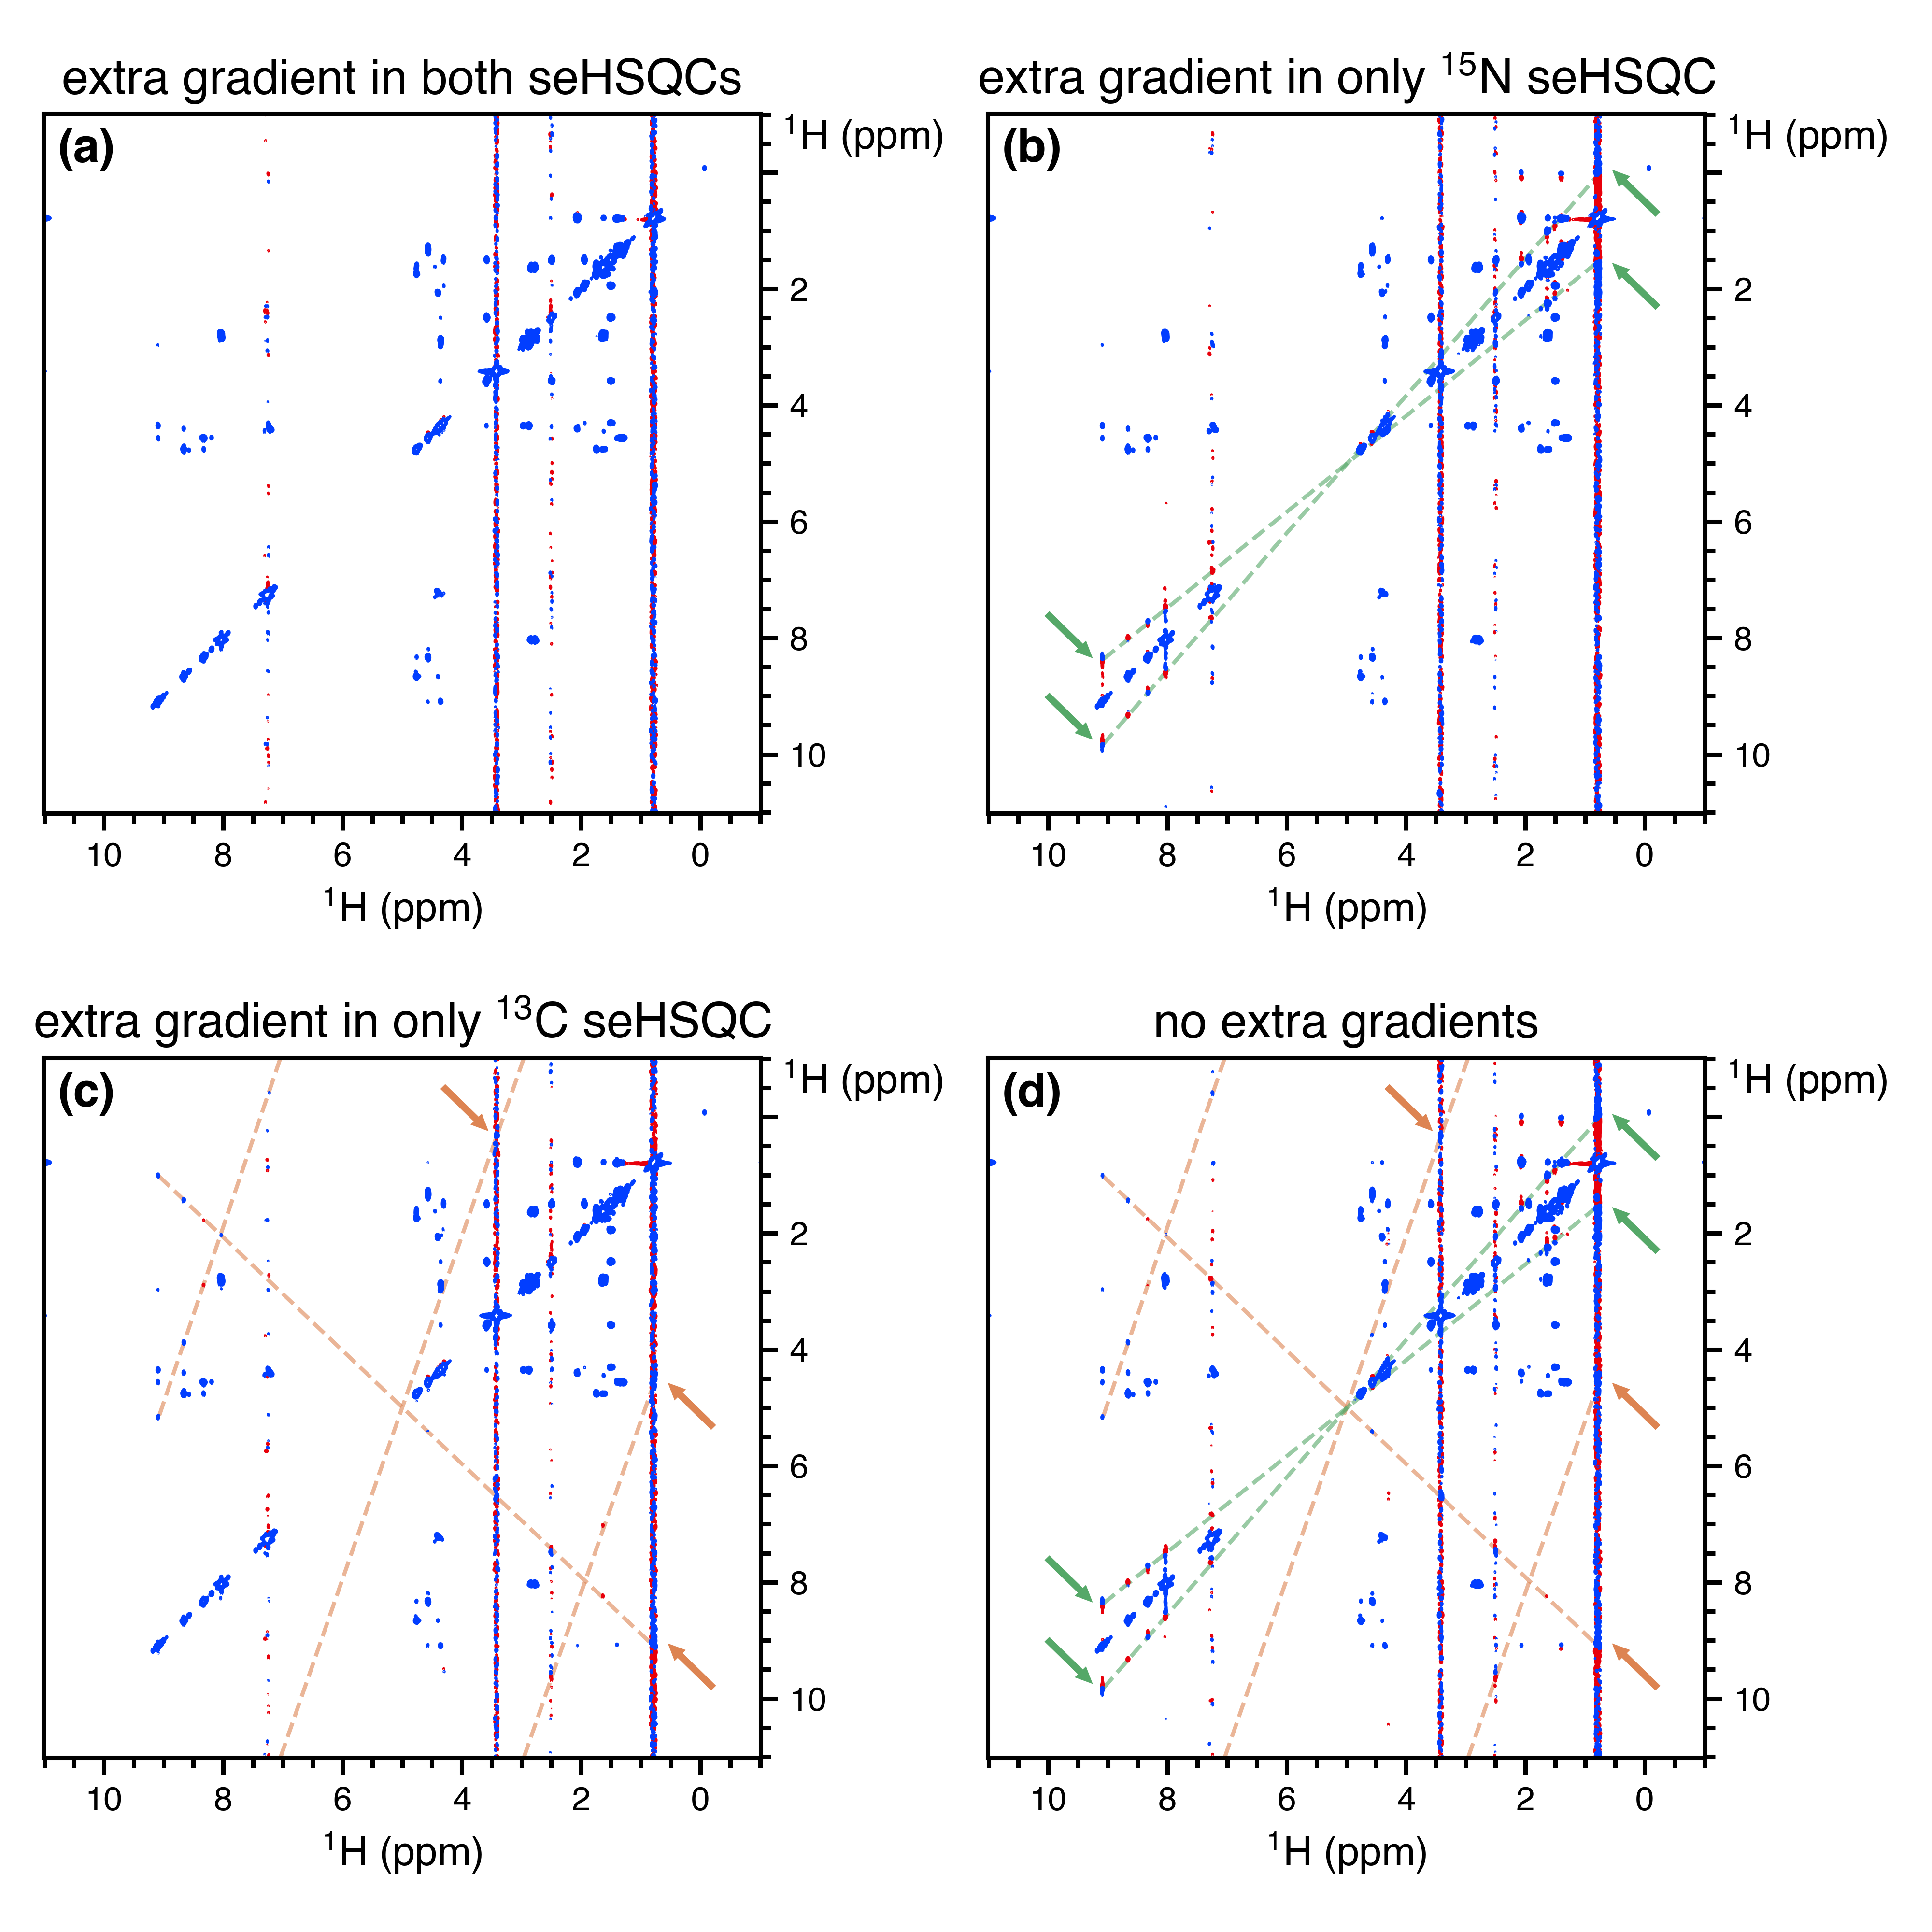
\includegraphics[width=0.8\textwidth]{wing_artefacts2.png}
    \caption{
        The same spectra as \cref{fig:wing_artefacts}, but plotted with a smaller base contour level to illustrate the regular indirect-dimension frequencies of the wing artefacts.
        A greater number of artefacts are now visible (in addition to those already highlighted in \cref{fig:wing_artefacts}, which are still marked with arrows).
        The artefacts arising from the \nitrogen{} seHSQC lie on the orange dotted line; those arising from the \carbon{} seHSQC lie on the green dotted line.
        \textbf{(a)} With the extra gradient inserted for both modules, i.e.\ no artefacts.
        \textbf{(b)} With an extra gradient in only the \nitrogen{} module, i.e.\ only the \carbon{} artefacts.
        \textbf{(c)} With an extra gradient in only the \carbon{} module.
        \textbf{(d)} With no extra gradients.
        \grami{}
    }
    \label{fig:wing_artefacts2}
\end{figure}

\clearpage

Additional information can be gleaned from the following series of CLIP-COSY spectra, obtained from NOAH-2 \noahtwo{Spb}{Cc} supersequences.
In the seHSQC module, the two gradients $g_1$ in the $t_1$ period are independently enabled or disabled (by setting their amplitude to 0).
Traces of the resulting CLIP-COSY spectra are shown in \cref{fig:wing_gradients}.
The gradients serve to dephase any bulk \magnnot{\ce{C}} magnetisation that is transverse during either half of $t_1$: therefore, if (for example) the gradient in the first half of $t_1$ is switched off, this allows bulk magnetisation that is transverse in the first half of $t_1$ to evolve and ultimately contribute to the wing artefacts in the CLIP-COSY.
As can be seen, gradients must be applied in \textit{both} halves for complete suppression of the wing artefacts.

\begin{figure}
    \centering
    
\includegraphics{andro.png}

    % figures/wing_gradients.py
    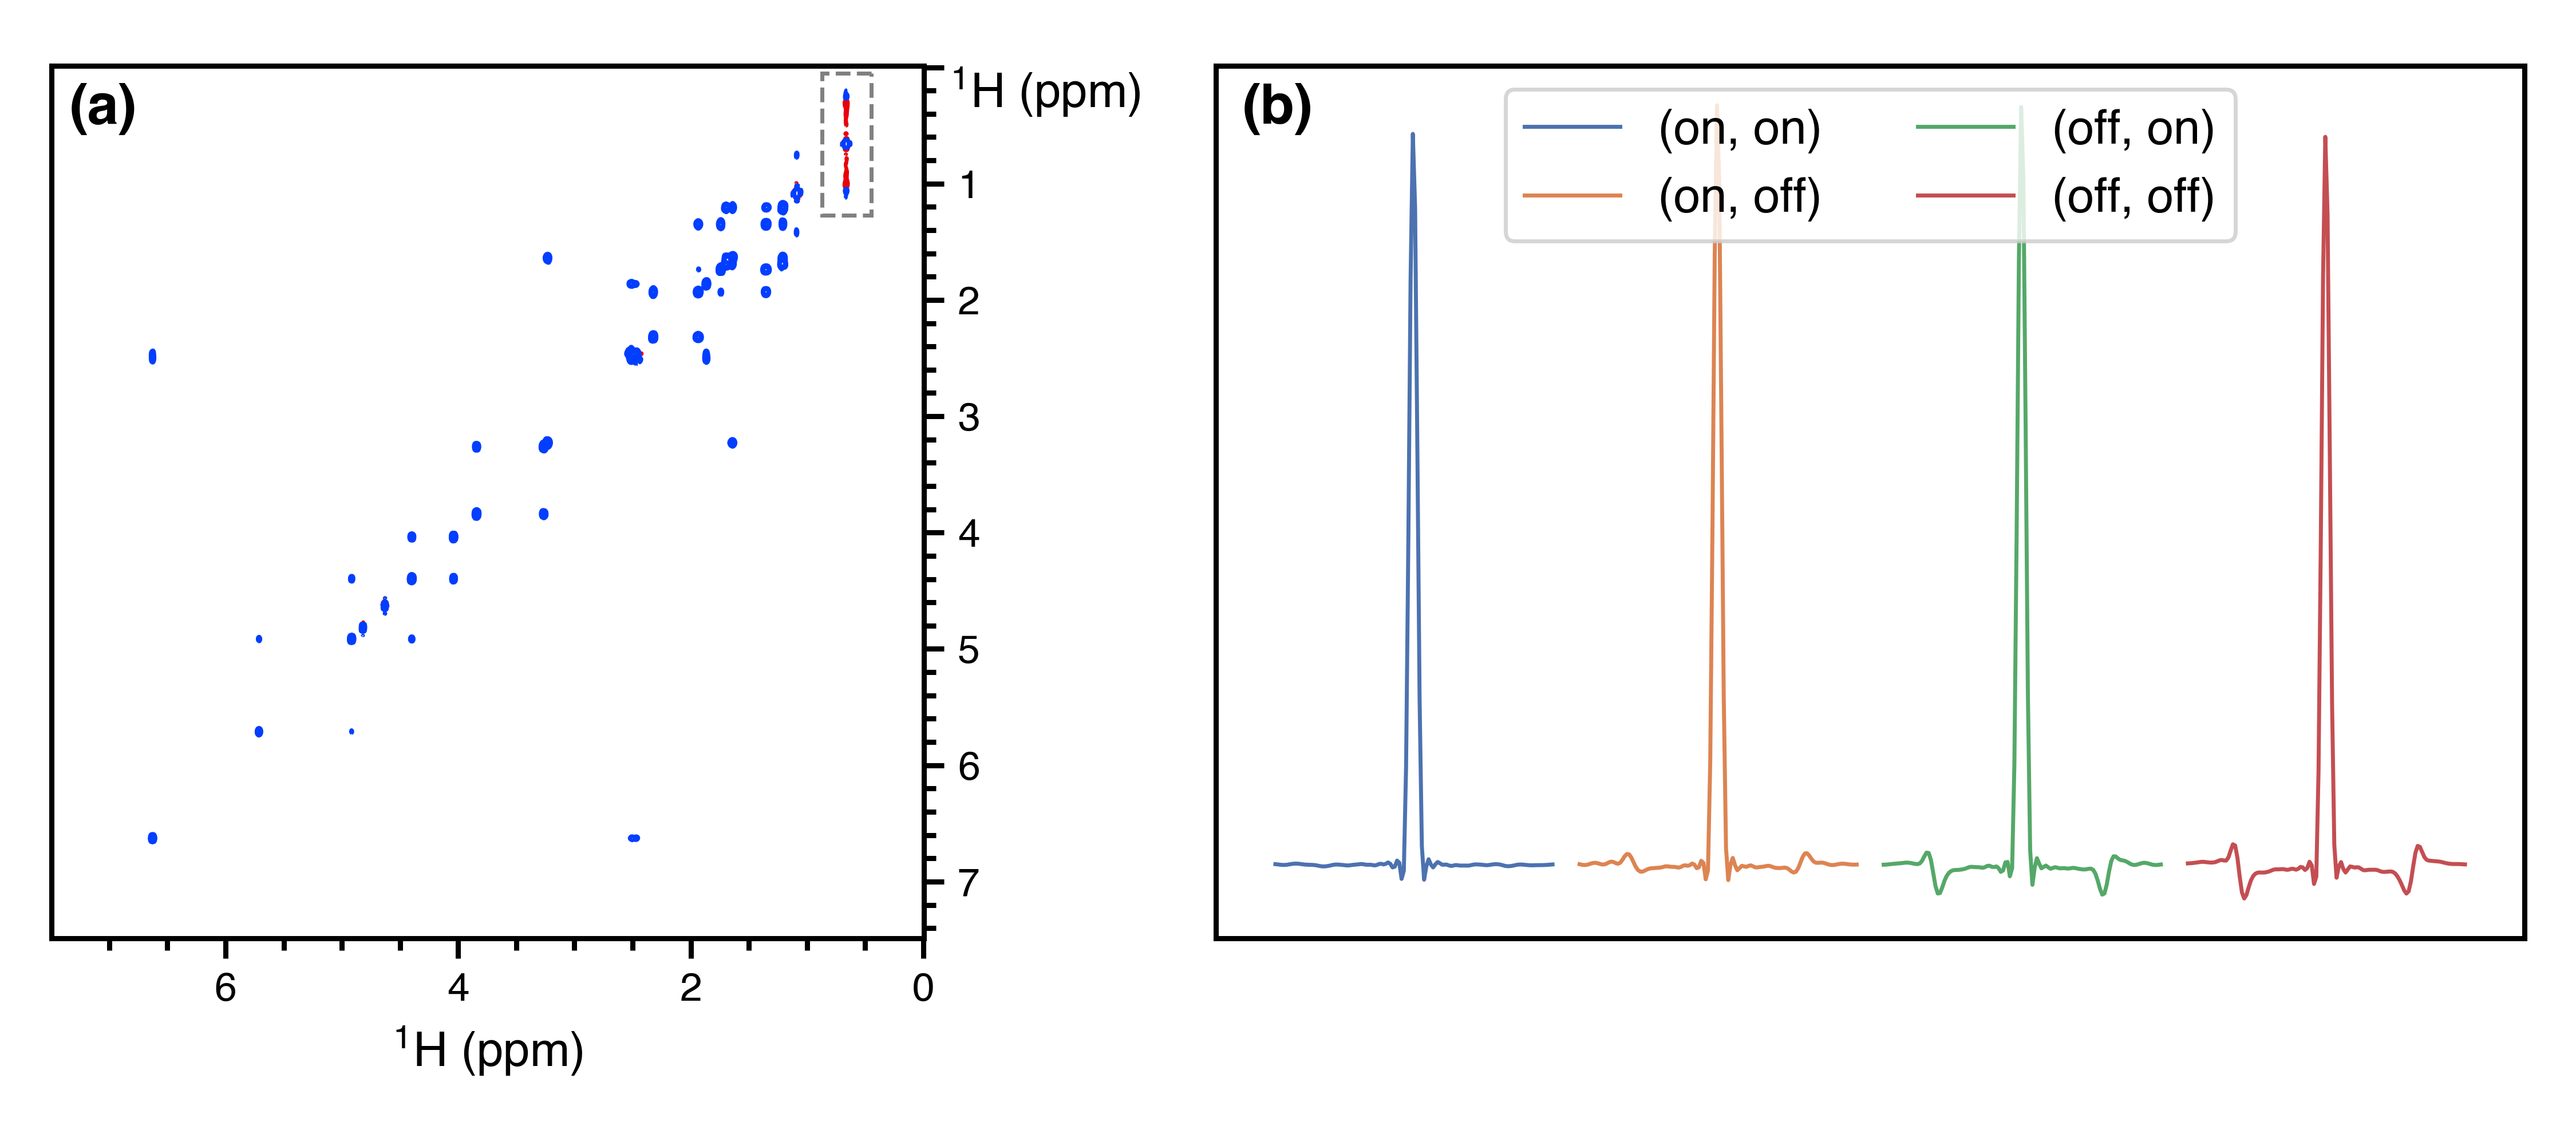
\includegraphics[width=0.8\textwidth]{wing_gradients.png}
    \caption{
        \textbf{(a)} CLIP-COSY spectrum obtained from NOAH-2 \noahtwo{Spb}{Cc} sequence, where both gradients in $t_1$ were disabled (i.e.\ ``(off, off)'').
        The other three CLIP-COSY spectra are similar, except that the (on, on) spectrum (with gradients applied in both halves of $t_1$) does not have wing artefacts (grey box).
        \textbf{(b)} $f_1$ traces through \SI{0.67}{\ppm} of the four CLIP-COSY spectra obtained with various combinations of gradients, corresponding to the boxed area in (a).
        Only the (on, on) spectrum (in blue) is free from wing artefacts.
        The (on, off) and (off, on) spectra (in orange and green respectively) have wing artefacts arising from bulk magnetisation that evolves during the second and first halves of the seHSQC $t_1$ period respectively.
        The (off, off) spectrum (red), which corresponds to the 2D spectrum in (a), has the greatest intensity of wing artefacts.
        \andro{}
    }
    \label{fig:wing_gradients}
\end{figure}

It is interesting to note that the evolution of magnetisation during multiple indirect dimensions is the basis of projection spectroscopy,\autocite{projrecon} where the resulting sums and differences of frequencies can be used to reconstruct higher-dimensional spectra.
In the present context, the aim is instead to suppress these peaks, permitting evolution to only occur in a single indirect dimension.


\section{Effect of setting \texorpdfstring{$\Delta' = 1/(4\cdot\onejch)$}{Delta' = 1/(4*1JCH)} in seHSQC}

\begin{figure}
    \centering
    % figures/1_4j_unedited.py
    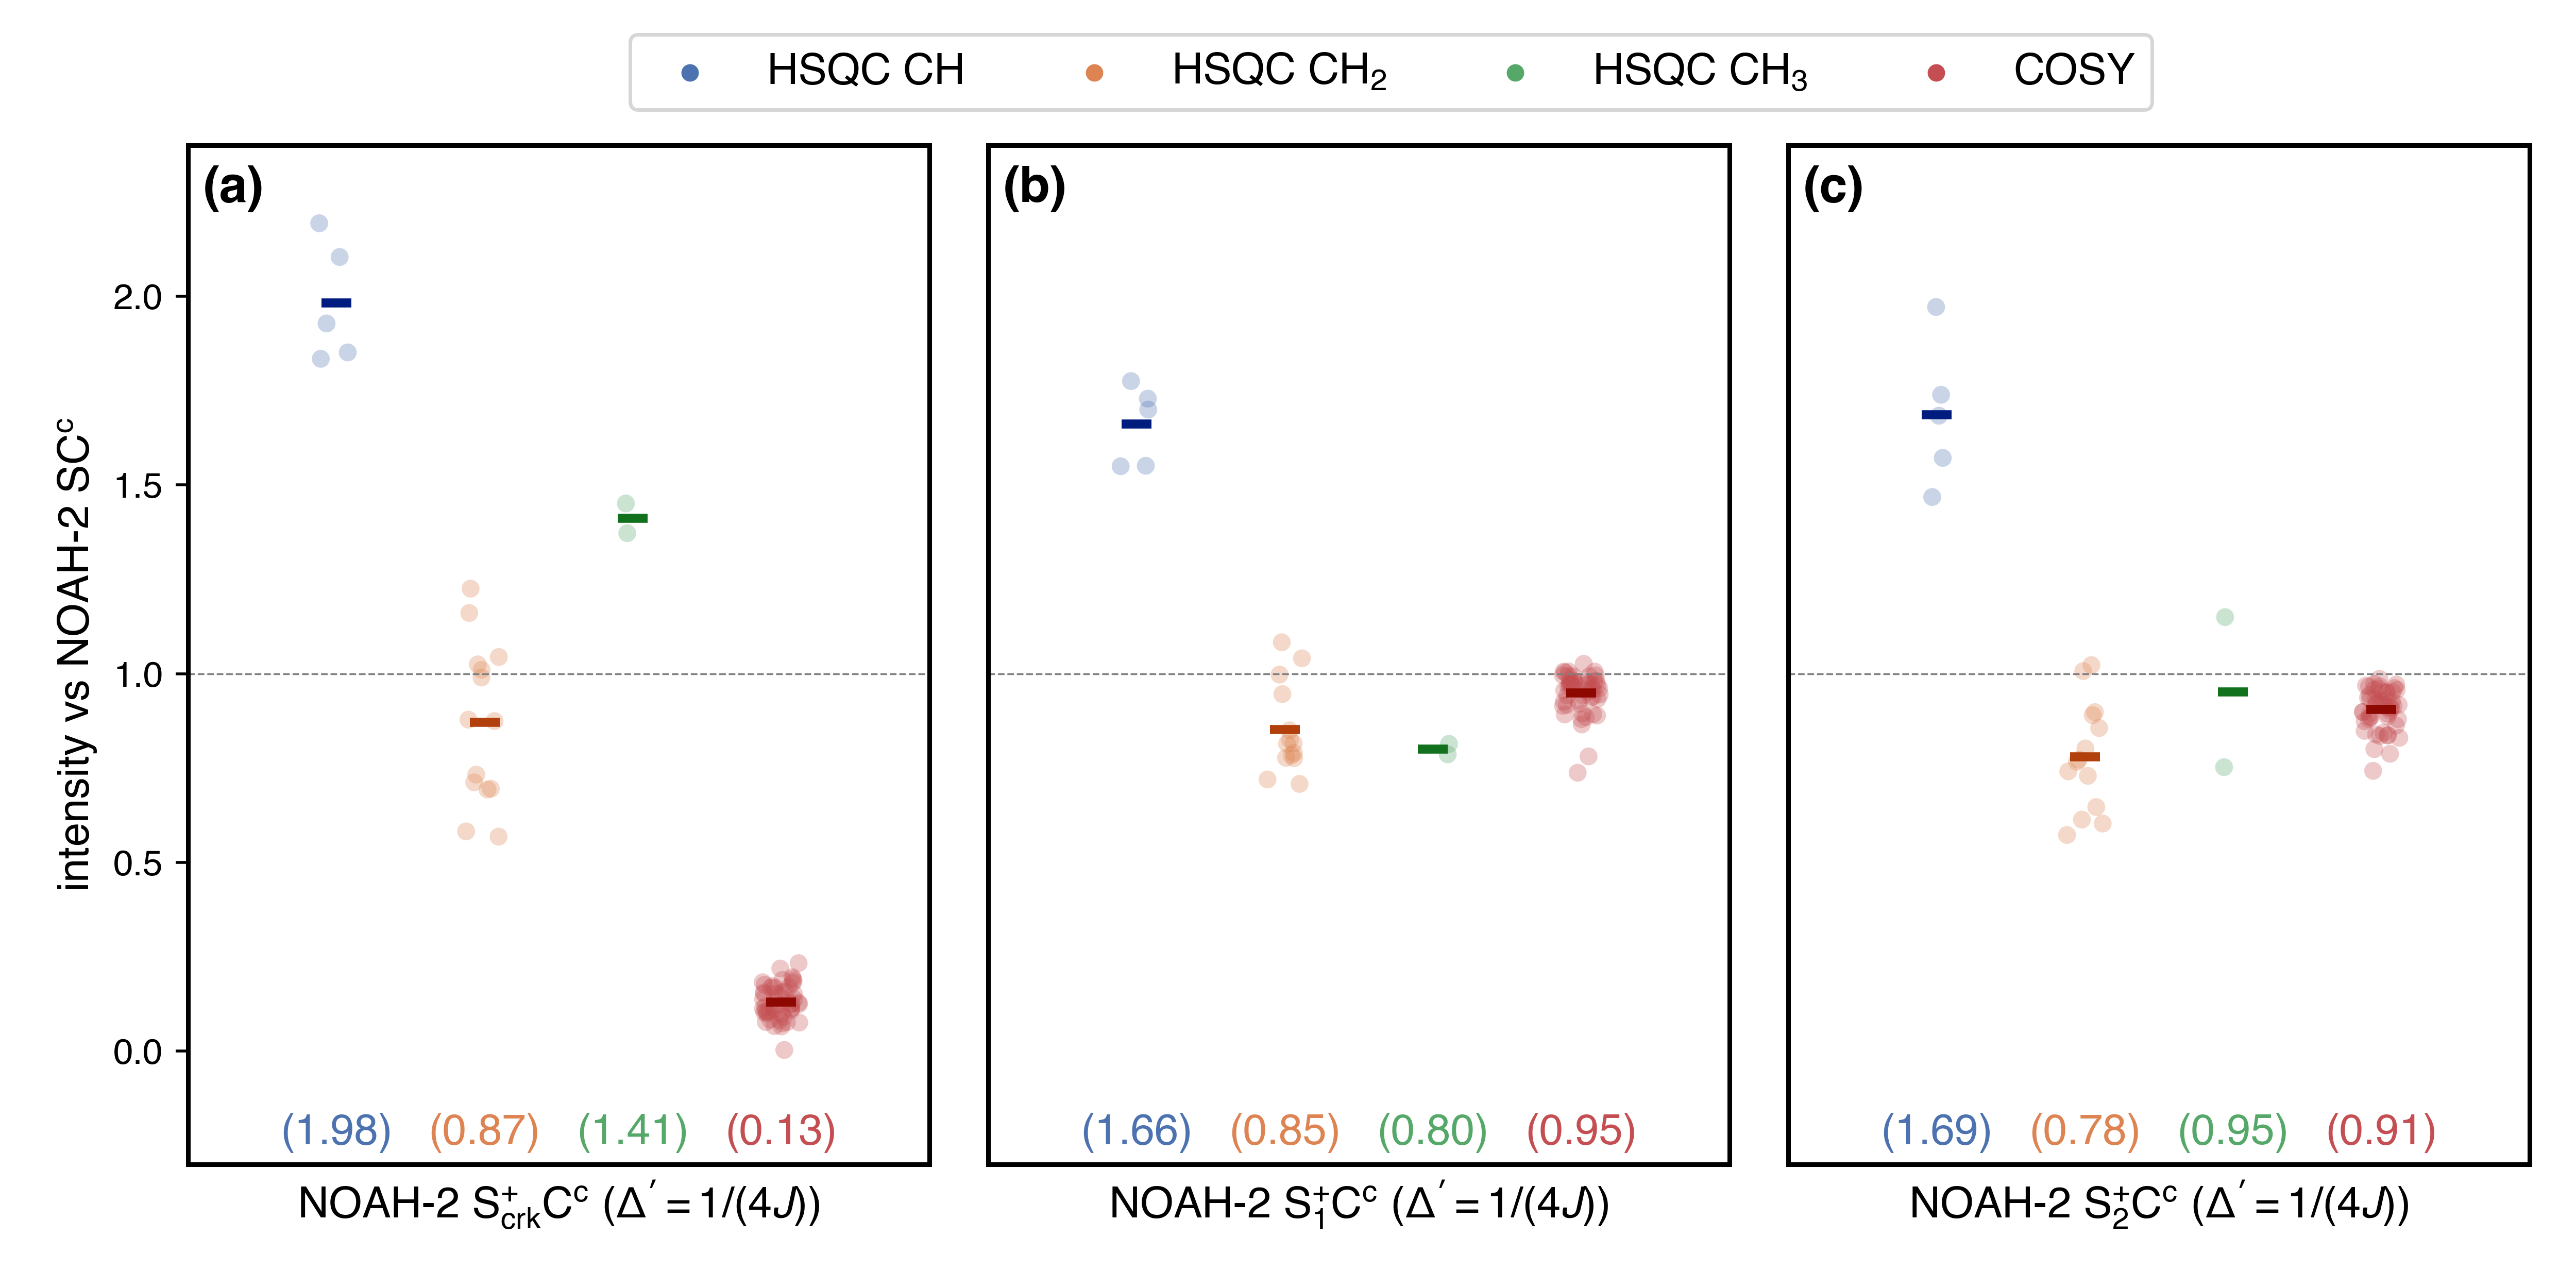
\includegraphics[width=0.9\textwidth]{1_4j_unedited.png}
    {\phantomsubcaption\label{fig:1_4j_unedited_crk}}
    {\phantomsubcaption\label{fig:1_4j_unedited_spv1}}
    {\phantomsubcaption\label{fig:1_4j_unedited_spv2}}
    \caption{
        Sensitivity of NOAH-2 \noahtwo{Sp}{Cc} supersequences with $\Delta'$ set to $1/(4\cdot\onejch)$, relative to the NOAH-2 \noahtwo{S}{Cc} supersequence.
        \textbf{\subref{fig:1_4j_unedited_crk}} Using the CRK seHSQC.
        \textbf{\subref{fig:1_4j_unedited_spv1}} Using the \noahSpa{} module.
        \textbf{\subref{fig:1_4j_unedited_spv2}} Using the \noahSpb{} module.
        \andro{}
    }
    \label{fig:1_4j_unedited}
\end{figure}

By setting $\Delta' = 1/(4\cdot\onejch)$, theory predicts a larger sensitivity enhancement for \ce{CH} peaks, whereas \ce{CH2} and \ce{CH3} peaks should have sensitivities comparable to the unenhanced HSQC.

Although the CRK seHSQC has slightly better performance over the NOAH seHSQCs, its major drawback remains in that it does not preserve any \magnnot{\ce{X}} magnetisation for a subsequent homonuclear module (\cref{fig:1_4j_unedited_crk}): the duration of $\Delta'$ chosen does not affect this in any way.
Thus, we limit our discussion to the two NOAH seHSQC variants (\cref{fig:1_4j_unedited_spv1,fig:1_4j_unedited_spv2}).
Both of these do indeed display the expected gains for \ce{CH} peaks: the corresponding sensitivities with $\Delta' = 1/(8\cdot\onejch)$ are shown in \cref{fig:sehsqc_comp}.
For \ce{CH2} and \ce{CH3} peaks, we observe sensitivity \textit{losses} even relative to the unenhanced HSQC; this is likely due to pulse imperfections in the longer pulse sequence and is in line with previous studies.\autocite{Schleucher1994JBNMR}
This is generally not desirable in a \carbon{} seHSQC, where \ce{CH2} peaks are common and are often further split due to diastereotopicity.
However, in the \nitrogen{} seHSQC, the delay $\Delta'$ can often be set to $1/(4\cdot\onejnh)$ to provide the maximum sensitivity enhancement for \ce{NH} peaks.

\begin{figure}[H]
    \centering
    % figures/1_4j_edited.py
    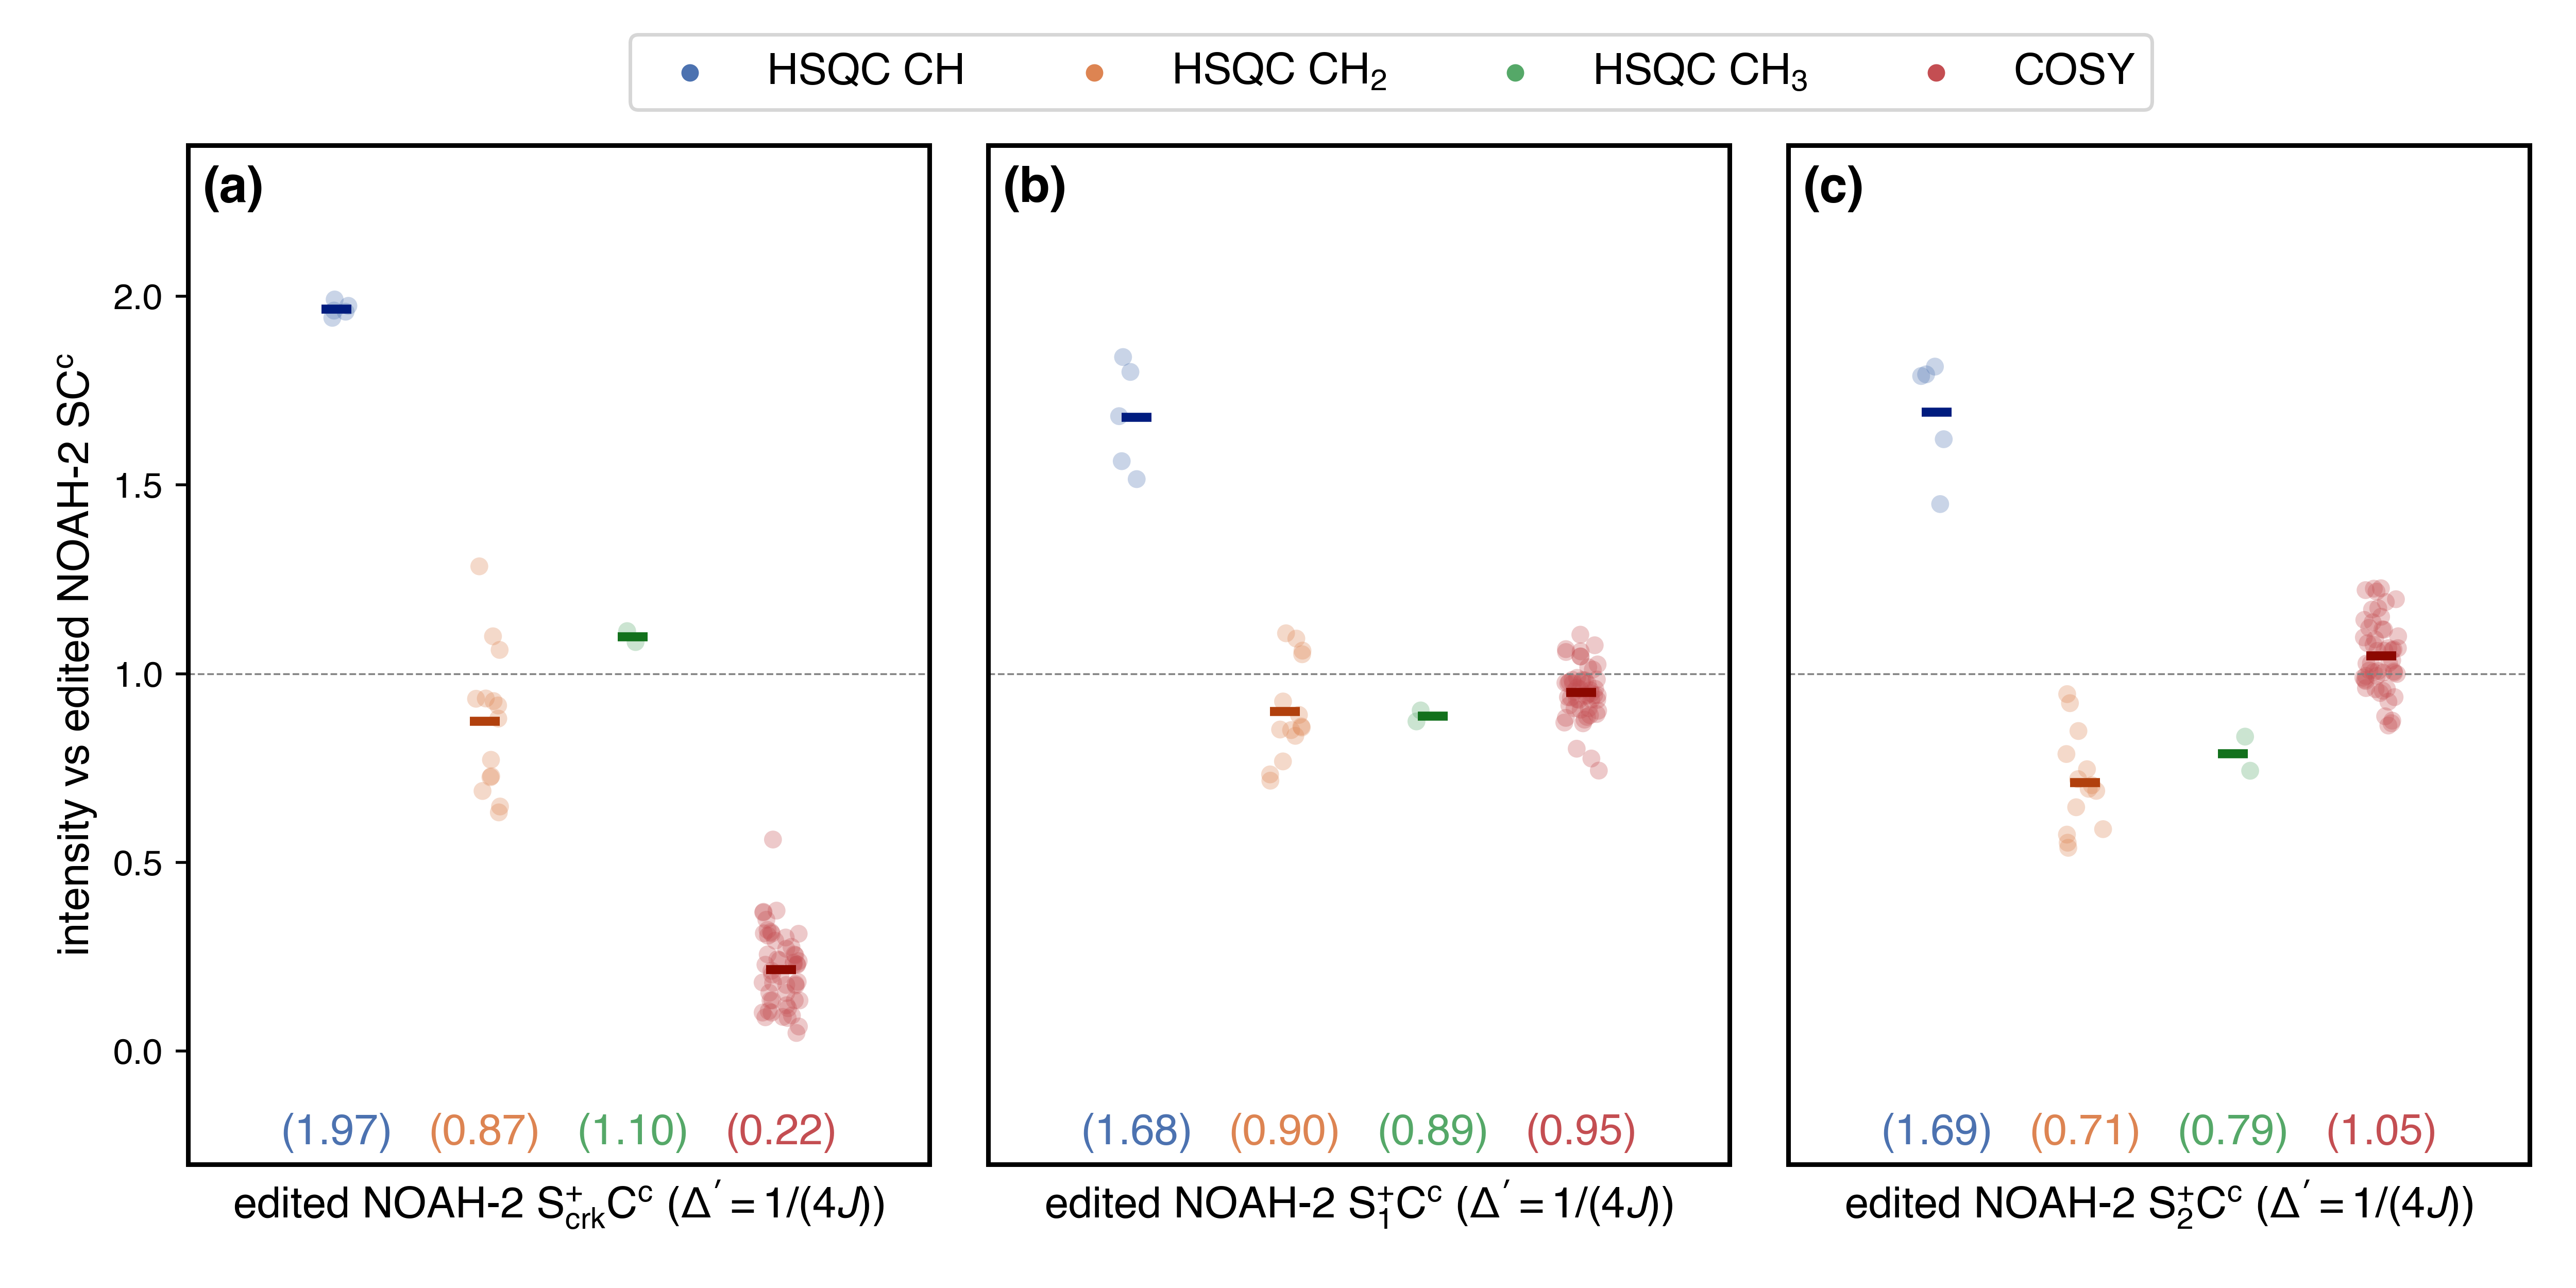
\includegraphics[width=0.9\textwidth]{1_4j_edited.png}
    {\phantomsubcaption\label{fig:1_4j_edited_crk}}
    {\phantomsubcaption\label{fig:1_4j_edited_spv1}}
    {\phantomsubcaption\label{fig:1_4j_edited_spv2}}
    \caption{
        Sensitivity of multiplicity-edited NOAH-2 \noahtwo{Sp}{Cc} supersequences with $\Delta'$ set to $1/(4\cdot\onejch)$, relative to the multiplicity-edited NOAH-2 \noahtwo{S}{Cc} supersequence.
        \textbf{\subref{fig:1_4j_edited_crk}} Using the CRK seHSQC.
        \textbf{\subref{fig:1_4j_edited_spv1}} Using the \noahSpa{} module.
        \textbf{\subref{fig:1_4j_edited_spv2}} Using the \noahSpb{} module.
        \andro{}
    }
    \label{fig:1_4j_edited}
\end{figure}

The inclusion of multiplicity editing in the sequences with $\Delta' = 1/(4\cdot\onejch)$ makes no substantial difference to the results (\cref{fig:1_4j_edited}), save for a slight relative improvement in the amount of \magnnot{\ce{X}} magnetisation preserved by the \noahSpb{} module.
The reasons for this are discussed in the main text.

\section{Comparison of BIG-BIRD and ZIP elements}

Following the formula of Briand and S\o{}rensen,\autocite{Briand1997JMR} the BIG-BIRD element used here was ${45^\circ}_{45^\circ}(\proton{}) - 2\Delta - 180^\circ(\proton{},\carbon{}) - 2\Delta - {45^\circ}_{225^\circ}(\proton{})$ for the unedited NOAH seHSQC, where $\beta_\phi$ indicates a hard pulse with flip angle $\beta$ and phase $\phi$, and $\Delta = 1/(4\cdot\onejch)$.
For the edited NOAH seHSQC, the BIG-BIRD pulse phases are slightly modified to give ${45^\circ}_{315^\circ}(\proton{}) - 2\Delta - 180^\circ(\proton{},\carbon{}) - 2\Delta - {45^\circ}_{135^\circ}(\proton{})$.
These, and the ZIP, have the same net effect on \magn{\ce{C}} and \magnnot{\ce{C}} magnetisation, as can be seen from the product operator analysis in \cref{fig:pprogs_prodop}.
Thus, they can be used interchangeably in version 2 of the NOAH seHSQC.
However, the ZIP provides greater sensitivity in both the HSQC and downstream COSY (\cref{fig:bigbird}).

\begin{figure}
    \centering
    % figures/bigbird.py
    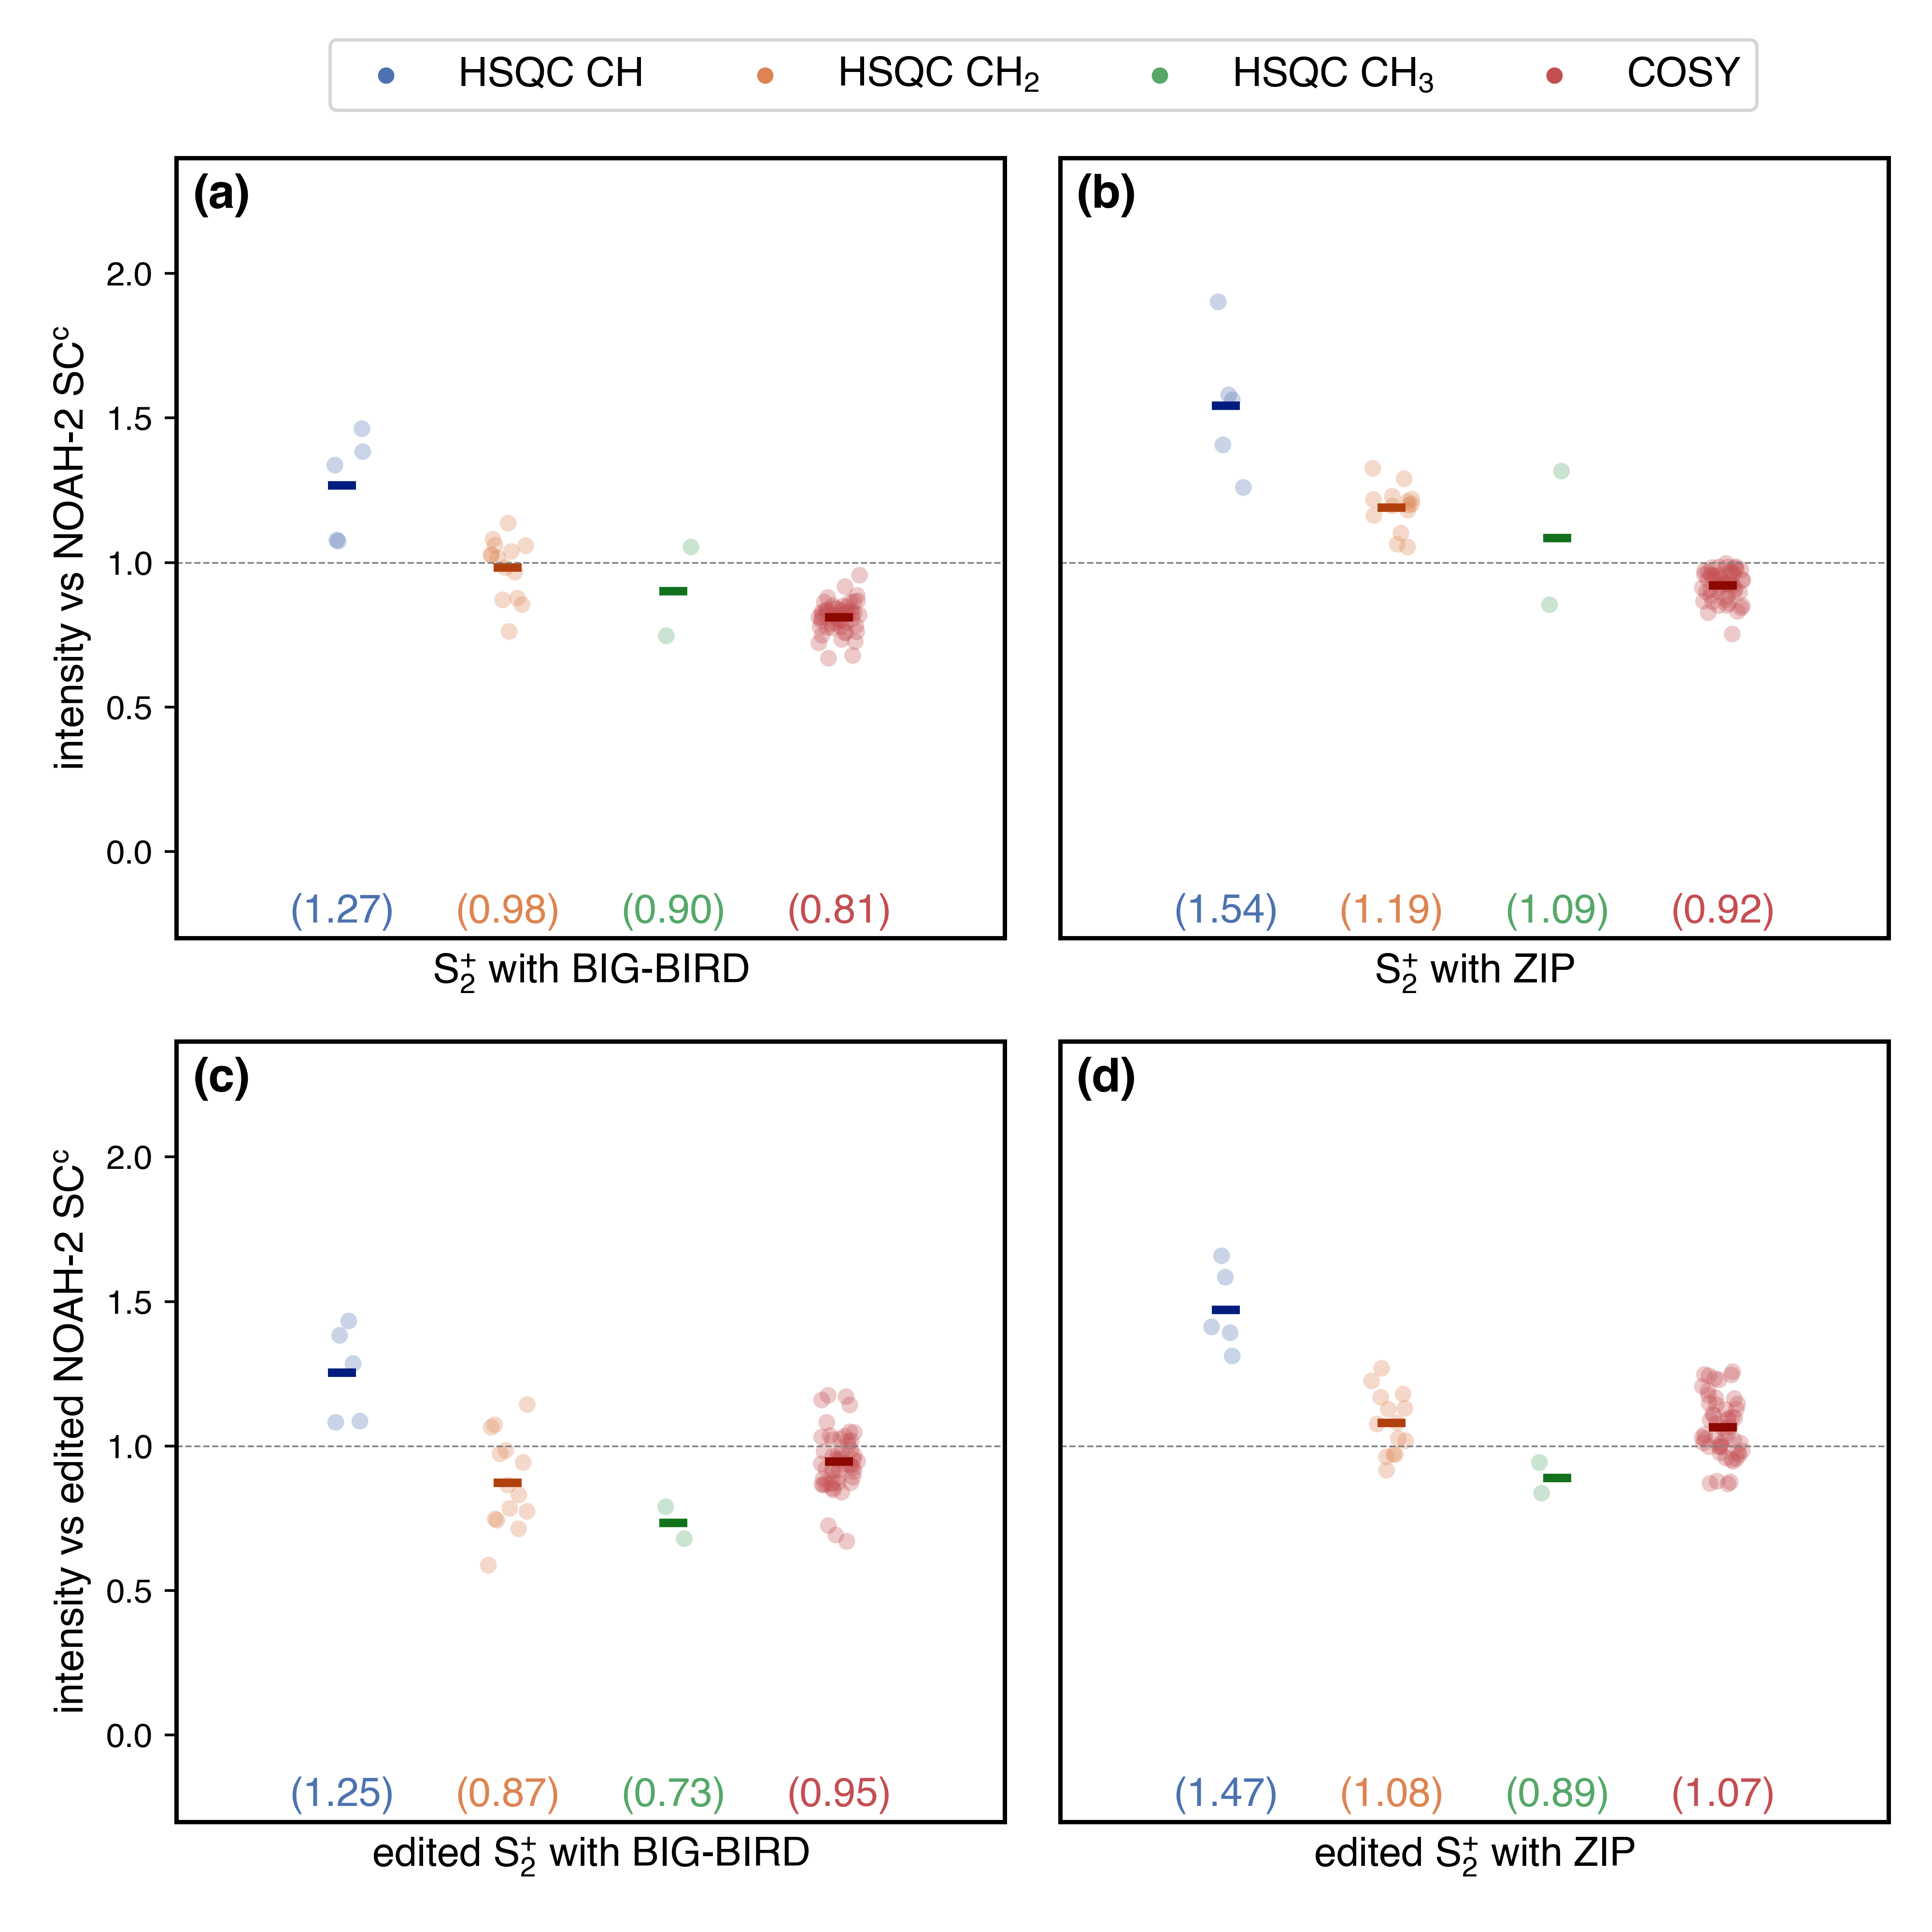
\includegraphics[width=0.8\textwidth]{bigbird.png}
    {\phantomsubcaption\label{fig:bigbird_unedited_bigbird}}
    {\phantomsubcaption\label{fig:bigbird_unedited_zip}}
    {\phantomsubcaption\label{fig:bigbird_edited_bigbird}}
    {\phantomsubcaption\label{fig:bigbird_edited_zip}}
    \caption{
        Sensitivity of NOAH-2 \noahtwo{Spb}{Cc} supersequences with either BIG-BIRD or ZIP elements, versus the corresponding NOAH-2 \noahtwo{S}{Cc} supersequences (i.e.\ unedited for (a) and (b), edited for (c) and (d)).
        The value of $\Delta'$ was set to $1/(8 \cdot \onejch)$.
        \textbf{\subref{fig:bigbird_unedited_bigbird}} Using the unedited NOAH seHSQC with the BIG-BIRD element.
        \textbf{\subref{fig:bigbird_unedited_zip}} Unedited seHSQC with ZIP.
        \textbf{\subref{fig:bigbird_edited_bigbird}} Edited seHSQC with BIG-BIRD.
        \textbf{\subref{fig:bigbird_edited_zip}} Edited seHSQC with ZIP.
        \andro{}
    }
    \label{fig:bigbird}
\end{figure}

Note that the BIG-BIRD element is a generalisation of the earlier TANGO\autocite{Wimperis1984JMR} and BANGO\autocite{Sorensen1994BMR} elements.
The latter two do not allow for excitation with variable phase, which makes them insufficient for the present purpose.

\section{Multiplicity editing in seHSQC}

\begin{figure}
    \centering
    % done in Inkscape
    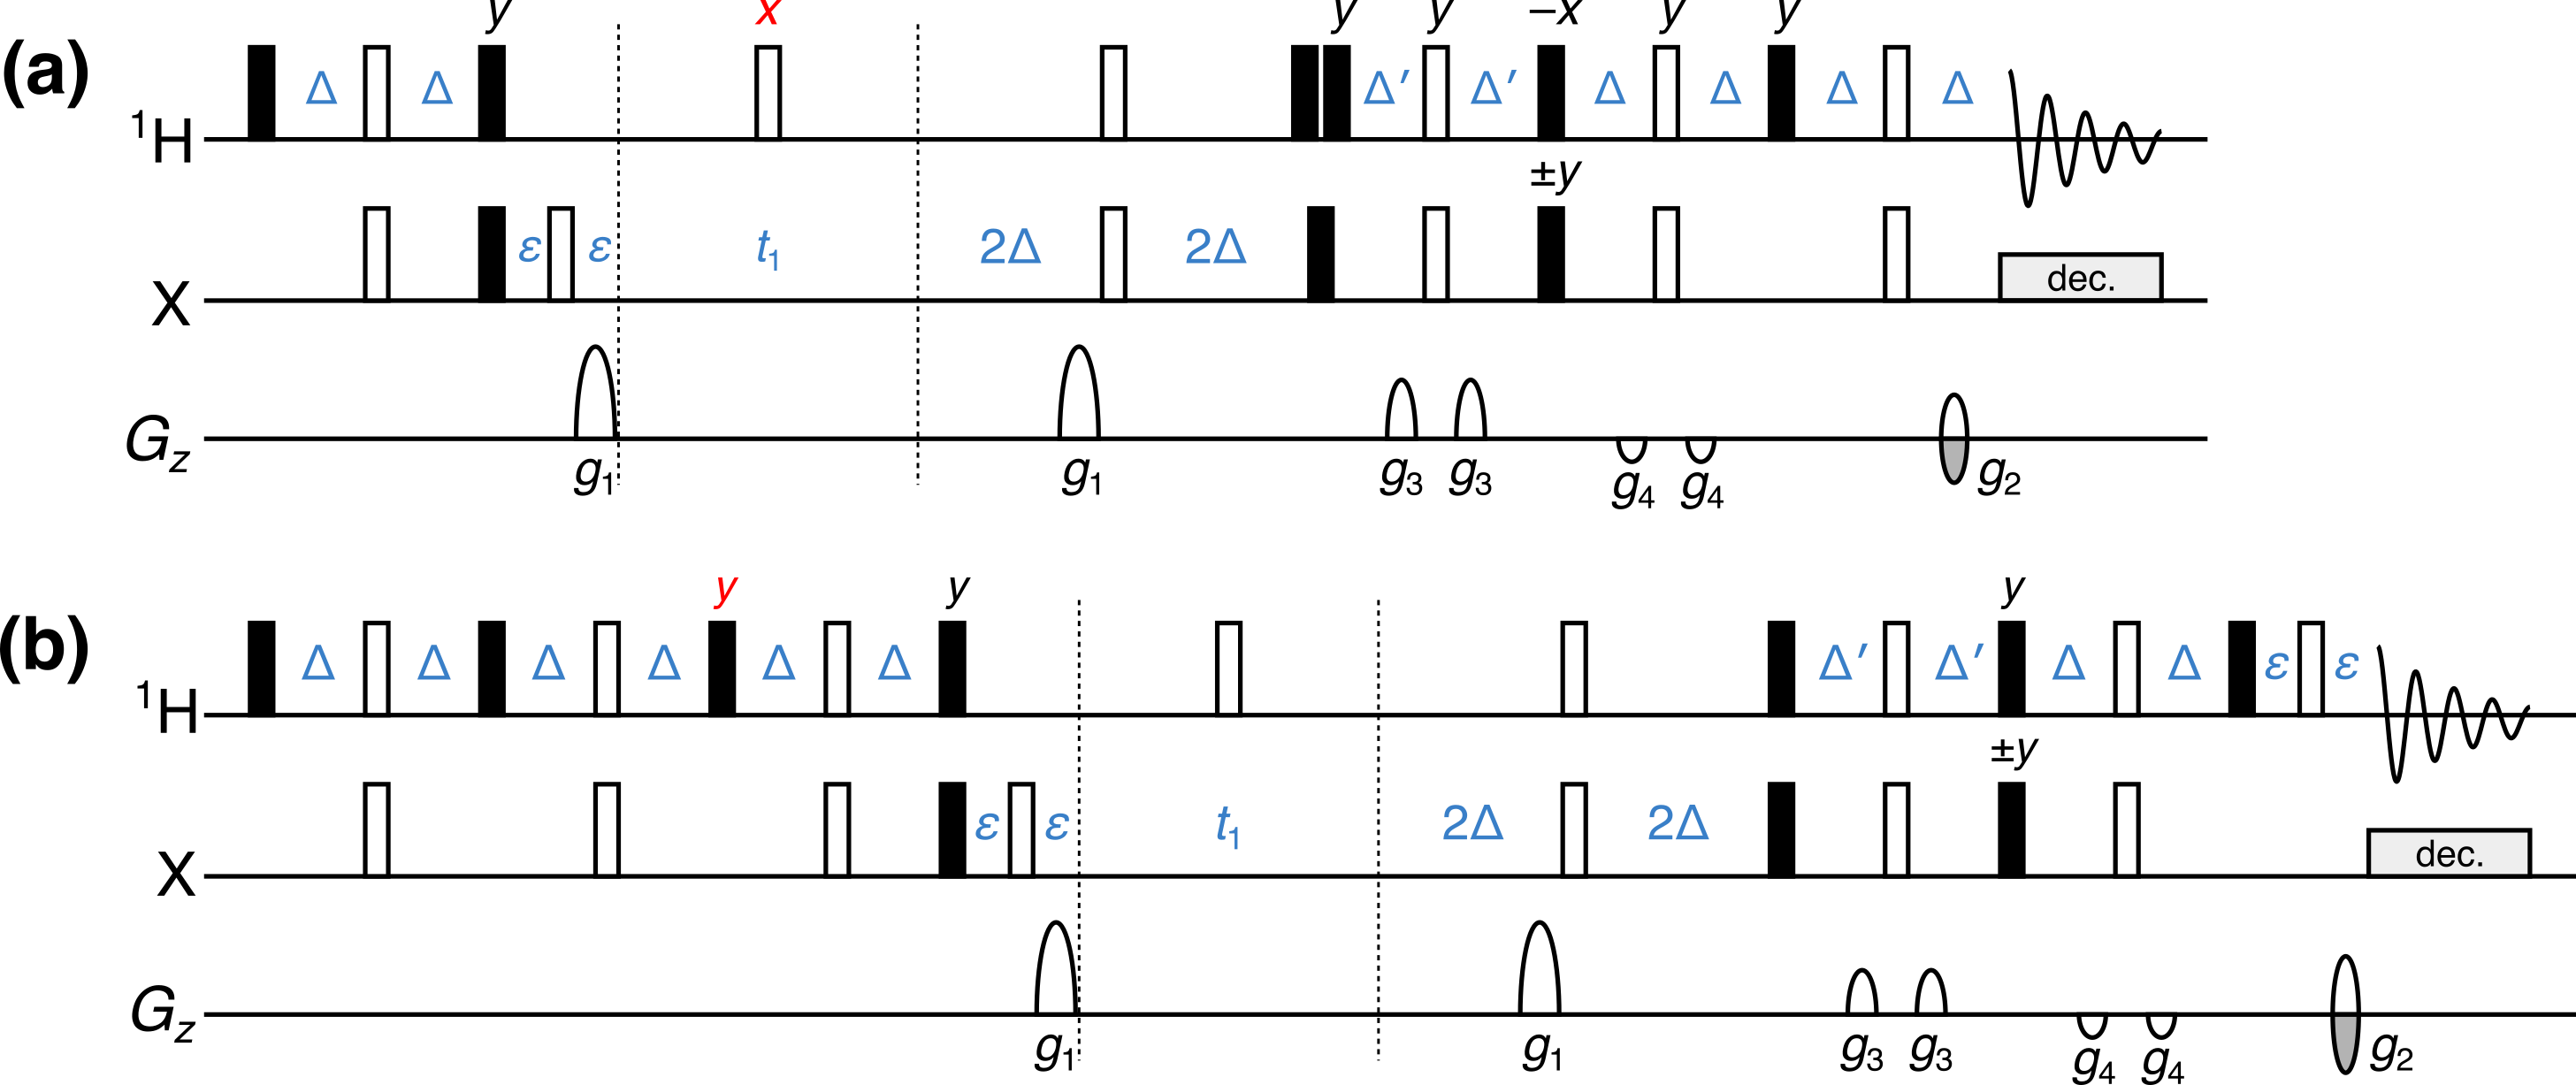
\includegraphics[width=0.8\textwidth]{mult_edit.png}
    {\phantomsubcaption\label{fig:mult_edit_spv1}}
    {\phantomsubcaption\label{fig:mult_edit_spv2}}
    \caption{
        Implementation of multiplicity editing in the new NOAH seHSQC modules.
        Pulse phases which differ from the unedited versions (\cref{fig:pprogs_prodop}) are highlighted in red; these are needed to compensate for the extra \proton{} \ang{180} pulse in the editing period.
        Symbols have the same meaning as in \cref{fig:pprogs} of the main text.
        \textbf{\subref{fig:mult_edit_spv1}} NOAH seHSQC, version 1 (``\noahSpa{}'').
        \textbf{\subref{fig:mult_edit_spv2}} NOAH seHSQC, version 2 (``\noahSpb{}'' / ZIP-seHSQC).
    }
    \label{fig:mult_edit}
\end{figure}

\begin{figure}
    \centering
    % figures/edited_sn_comp.py
    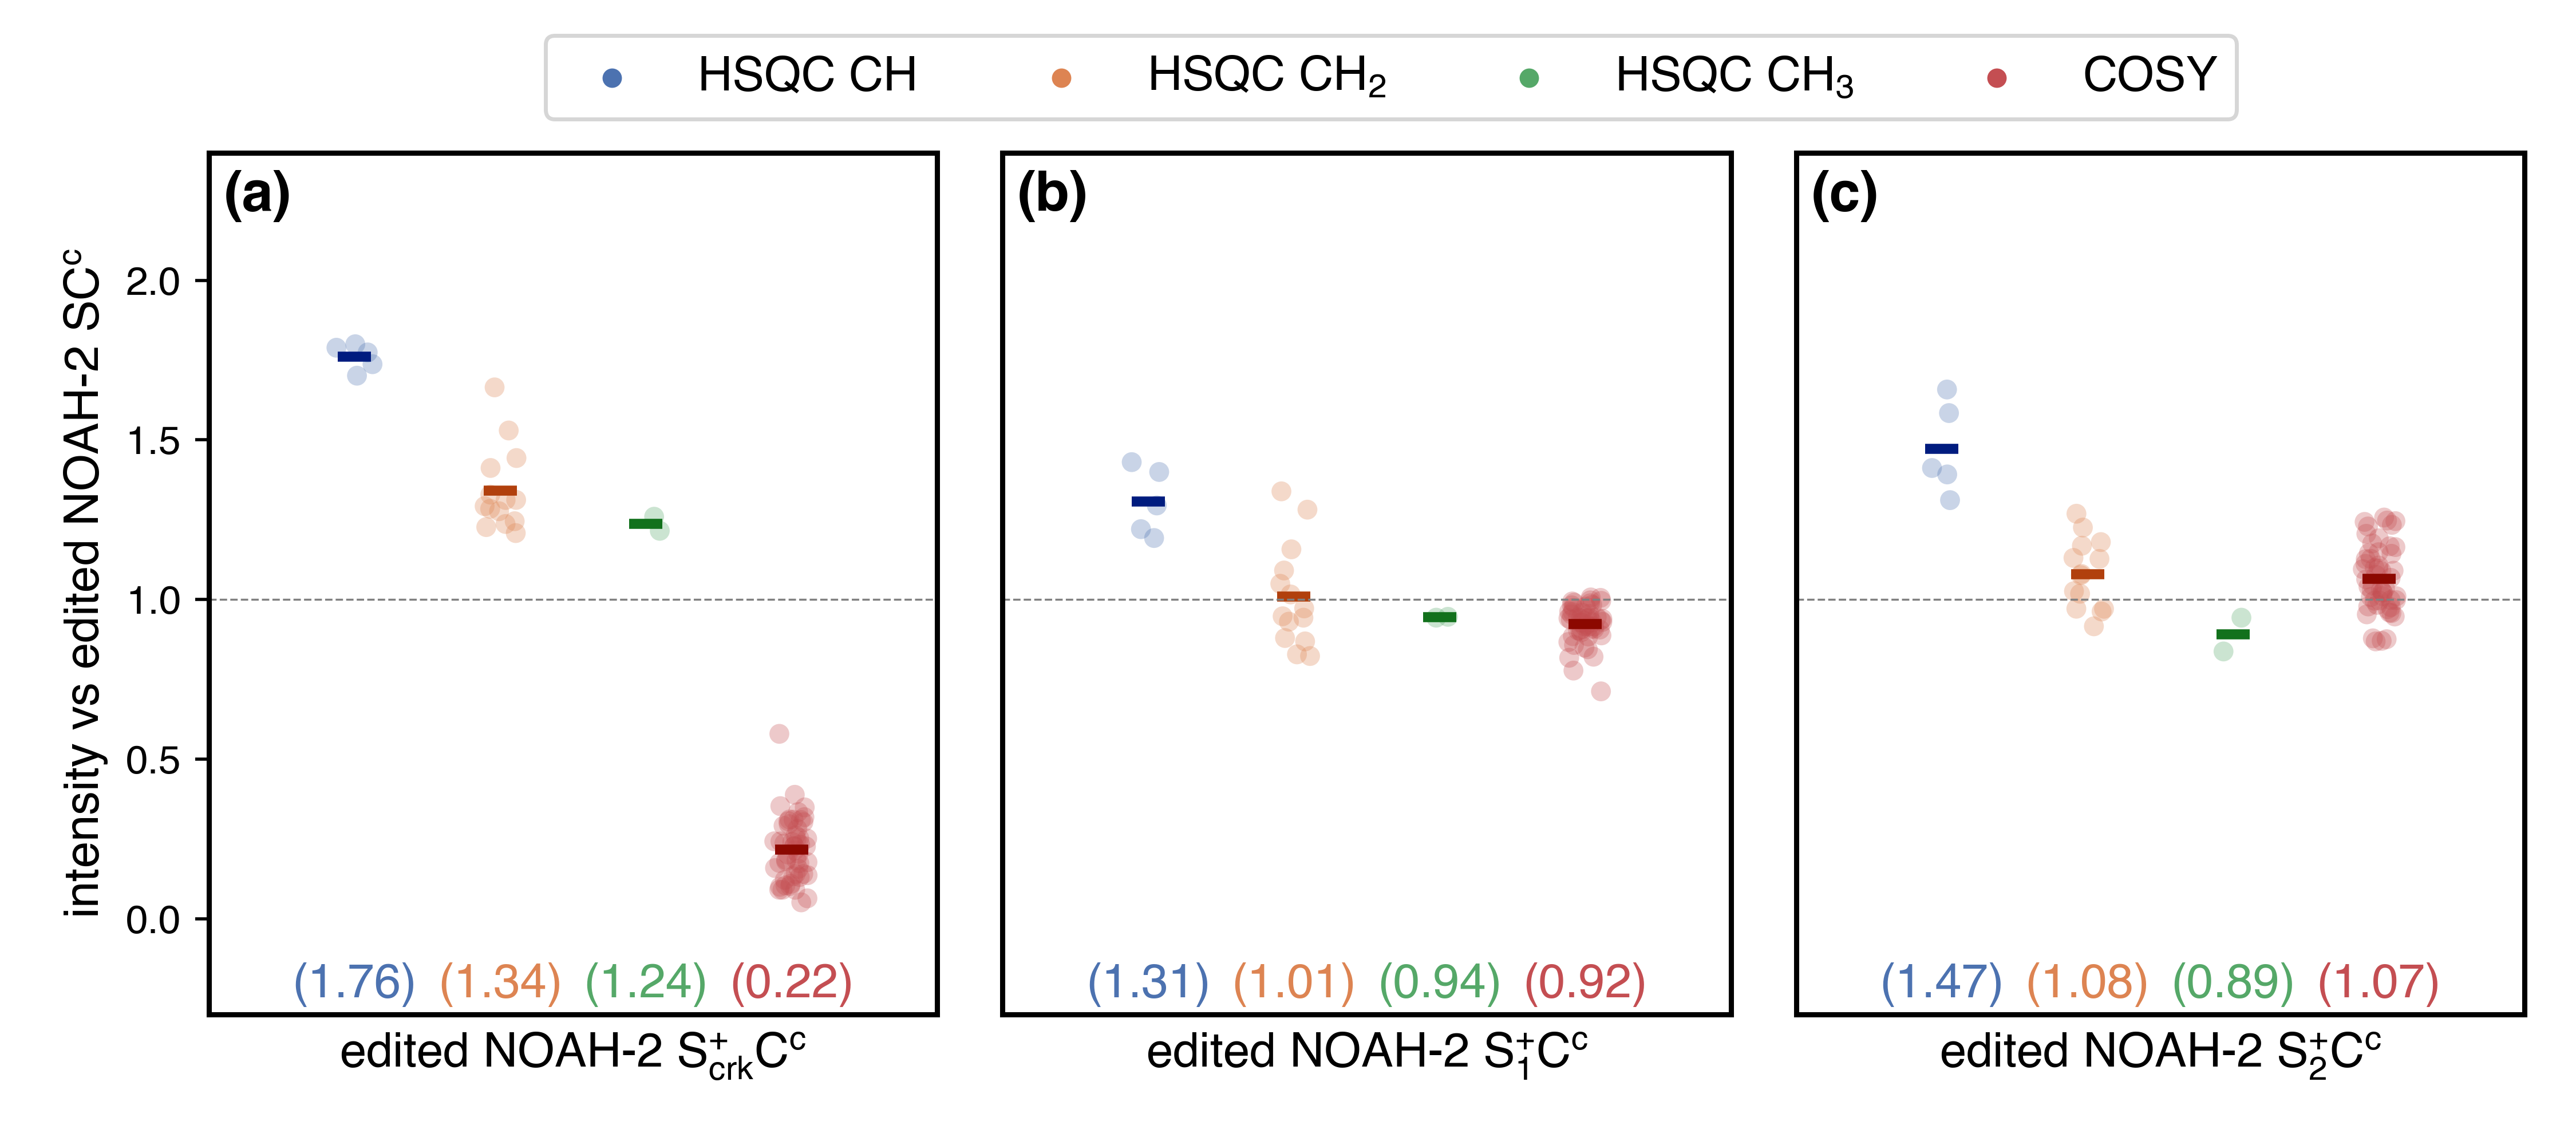
\includegraphics[width=0.9\textwidth]{edited_sn_comp.png}
    {\phantomsubcaption\label{fig:edited_sn_comp_crk}}
    {\phantomsubcaption\label{fig:edited_sn_comp_spv1}}
    {\phantomsubcaption\label{fig:edited_sn_comp_spv2}}
    \caption{
        Sensitivity of multiplicity-edited \noahtwo{Sp}{Cc} supersequences, relative to the \noahtwo{S}{Cc} supersequence.
        Spectra were obtained with $\Delta' = 1/(8\cdot\onejch)$.
        \textbf{\subref{fig:edited_sn_comp_crk}} Using the CRK seHSQC.
        \textbf{\subref{fig:edited_sn_comp_spv1}} Using the \noahSpa{} module.
        \textbf{\subref{fig:edited_sn_comp_spv2}} Using the \noahSpb{} module.
        \andro{}
    }
    \label{fig:edited_sn_comp}
\end{figure}

On average, both versions of the NOAH seHSQC provide sensitivity gains for HSQC \ce{CH} and \ce{CH2} peaks (\cref{fig:edited_sn_comp_spv1,fig:edited_sn_comp_spv2}) while not compromising the COSY intensities as the CRK seHSQC does (\cref{fig:edited_sn_comp_crk}).
The \noahSpb{} module in particular provides slightly better performance.
Note also how the COSY intensities with the \noahSpb{} module are on average higher than with the original HSQC module: this indicates that the \noahSpb{} module preserves bulk \magnnot{\ce{C}} magnetisation better.
As discussed in the main text, this is because the bulk magnetisation is longitudinal during the editing period.

\section{Summary of \texorpdfstring{\carbon{}}{13C} seHSQC sensitivity comparisons}

{ % tbl:sehsqc_comp {{{2
\renewcommand{\arraystretch}{1.1}
\begin{table}
    % to get the numbers, run sehsqc_summary.py
    \centering
    \begin{tabular}{clcccccc}
        \toprule
        \multicolumn{3}{c}{\textbf{Experiment}} & \multicolumn{3}{c}{\textbf{HSQC}} & \textbf{COSY} & \textbf{Figure} \\
        edited? & HSQC variant & $\Delta'$      & \ce{CH} & \ce{CH2} & \ce{CH3}     &               \\
        \midrule
        \multirow{8}{*}{no}
         & HSQC                & --             & \phantom{*}1.00* & \phantom{*}1.00* & \phantom{*}1.00* & \phantom{*}1.00* & -- \\
         & CRK seHSQC          & $1/(8J)$       & 1.80 & 1.32 & 1.58 & 0.13 & \labelcref{fig:sehsqc_comp_crk} \\
         & NOAH seHSQC v1      & $1/(8J)$       & 1.29 & 0.94 & 0.89 & 0.94 & \labelcref{fig:sehsqc_comp_spv1} \\
         & NOAH seHSQC v2      & $1/(8J)$       & 1.54 & 1.19 & 1.09 & 0.92 & \labelcref{fig:sehsqc_comp_spv2} \\
         & CRK seHSQC          & $1/(4J)$       & 1.98 & 0.87 & 1.41 & 0.13 & \labelcref{fig:1_4j_unedited_crk} \\
         & NOAH seHSQC v1      & $1/(4J)$       & 1.66 & 0.85 & 0.80 & 0.95 & \labelcref{fig:1_4j_unedited_spv1} \\
         & NOAH seHSQC v2      & $1/(4J)$       & 1.69 & 0.78 & 0.95 & 0.91 & \labelcref{fig:1_4j_unedited_spv2} \\
         & no HSQC, only COSY  & --             & --   & --   & --   & 1.09 & -- \\ 
        \midrule
        \multirow{8}{*}{yes}
         & HSQC                & --             & \phantom{$^\dagger$}1.00$^\dagger$ & \phantom{$^\dagger$}1.00$^\dagger$ & \phantom{$^\dagger$}1.00$^\dagger$ & \phantom{$^\dagger$}1.00$^\dagger$ & -- \\
         & CRK seHSQC          & $1/(8J)$       & 1.76 & 1.34 & 1.24 & 0.22 & \labelcref{fig:edited_sn_comp_crk} \\
         & NOAH seHSQC v1      & $1/(8J)$       & 1.31 & 1.01 & 0.94 & 0.92 & \labelcref{fig:edited_sn_comp_spv1} \\
         & NOAH seHSQC v2      & $1/(8J)$       & 1.47 & 1.08 & 0.89 & 1.07 & \labelcref{fig:edited_sn_comp_spv2} \\
         & CRK seHSQC          & $1/(4J)$       & 1.97 & 0.87 & 1.10 & 0.22 & \labelcref{fig:1_4j_edited_crk} \\
         & NOAH seHSQC v1      & $1/(4J)$       & 1.68 & 0.90 & 0.89 & 0.95 & \labelcref{fig:1_4j_edited_spv1} \\
         & NOAH seHSQC v2      & $1/(4J)$       & 1.69 & 0.71 & 0.79 & 1.05 & \labelcref{fig:1_4j_edited_spv2} \\
         & no HSQC, only COSY  & --             & --   & --   & --   & 1.29 & -- \\ 
        \bottomrule
    \end{tabular}
    \caption{
        Relative sensitivities of HSQC and CLIP-COSY spectra in NOAH-2 \noahtwo{S}{Cc} and \noahtwo{Sp}{Cc} supersequences.
        All sensitivities are normalised against the corresponding \noahtwo{S}{Cc} sequences: in particular, the unedited seHSQC supersequences are compared against the unedited \noahtwo{S}{Cc} (marked with *), and likewise edited seHSQC supersequences are compared against the edited \noahtwo{S}{Cc} (marked with $^\dagger$).
        Note that the two standalone CLIP-COSY entries (the last row in both sections) refer to the same spectrum, and therefore have the same \textit{absolute} sensitivity.
        The difference in the \textit{relative} sensitivity arises only because they are being compared against the COSY intensities in different reference supersequences, which is done here for consistency with the other figures in this text.
        See \cref{tbl:sehsqc_comp_cosy} for a version of this table where the COSY sensitivities in both unedited and edited supersequences are normalised against the standalone CLIP-COSY.
        \andro{}
    }
    \label{tbl:sehsqc_comp}
\end{table}
} % }}}2

{ % tbl:sehsqc_comp_cosy {{{2
\renewcommand{\arraystretch}{1.1}
\begin{table}
    % to get the numbers, run sehsqc_summary2.py
    \centering
    \begin{tabular}{clccccc}
        \toprule
        \multicolumn{3}{c}{\textbf{Experiment}} & \multicolumn{3}{c}{\textbf{HSQC}} & \textbf{COSY} \\
        edited? & HSQC variant & $\Delta'$      & \ce{CH} & \ce{CH2} & \ce{CH3}     &               \\
        \midrule
        \multirow{8}{*}{no}
         & HSQC                & --             & \phantom{*}1.00* & \phantom{*}1.00* & \phantom{*}1.00* & 0.93 \\
         & CRK seHSQC          & $1/(8J)$       & 1.80 & 1.32 & 1.58 & 0.12 \\
         & NOAH seHSQC v1      & $1/(8J)$       & 1.29 & 0.94 & 0.89 & 0.88 \\
         & NOAH seHSQC v2      & $1/(8J)$       & 1.54 & 1.19 & 1.09 & 0.85 \\
         & CRK seHSQC          & $1/(4J)$       & 1.98 & 0.87 & 1.41 & 0.12 \\
         & NOAH seHSQC v1      & $1/(4J)$       & 1.66 & 0.85 & 0.80 & 0.88 \\
         & NOAH seHSQC v2      & $1/(4J)$       & 1.69 & 0.78 & 0.95 & 0.84 \\
         & no HSQC, only COSY  & --             & --   & --   & --   & \phantom{$^\ddagger$}1.00$^\ddagger$ \\ 
        \midrule
        \multirow{8}{*}{yes}
         & HSQC                & --             & \phantom{$^\dagger$}1.00$^\dagger$ & \phantom{$^\dagger$}1.00$^\dagger$ & \phantom{$^\dagger$}1.00$^\dagger$ & 0.79 \\
         & CRK seHSQC          & $1/(8J)$       & 1.76 & 1.34 & 1.24 & 0.17 \\
         & NOAH seHSQC v1      & $1/(8J)$       & 1.31 & 1.01 & 0.94 & 0.73 \\
         & NOAH seHSQC v2      & $1/(8J)$       & 1.47 & 1.08 & 0.89 & 0.84 \\
         & CRK seHSQC          & $1/(4J)$       & 1.97 & 0.87 & 1.10 & 0.17 \\
         & NOAH seHSQC v1      & $1/(4J)$       & 1.68 & 0.90 & 0.89 & 0.75 \\
         & NOAH seHSQC v2      & $1/(4J)$       & 1.69 & 0.71 & 0.79 & 0.82 \\
         & no HSQC, only COSY  & --             & --   & --   & --   & \phantom{$^\ddagger$}1.00$^\ddagger$ \\ 
        \bottomrule
    \end{tabular}
    \caption{
        Relative sensitivities of HSQC and CLIP-COSY spectra in NOAH-2 \noahtwo{S}{Cc} and \noahtwo{Sp}{Cc} supersequences.
        All HSQC sensitivities are normalised against the HSQC spectrum in the corresponding \noahtwo{S}{Cc} sequences: in particular, the unedited seHSQCs are compared against the unedited HSQC (marked with *), and likewise edited seHSQCs are compared against the edited HSQC (marked with $^\dagger$).
        All COSY sensitivites are compared against the standalone CLIP-COSY spectrum (the last row in both sections, marked with $^\ddagger$).
        This is different from the figures used in this text, which compare the COSY intensities against the COSY component of the corresponding \noahtwo{S}{Cc} supersequence.
        See \cref{tbl:sehsqc_comp} for a version of this table which is consistent with the other figures in this text.
        \andro{}
    }
    \label{tbl:sehsqc_comp_cosy}
\end{table}
} % }}}2

\clearpage

\section{Retention of bulk magnetisation by \texorpdfstring{\nitrogen{}}{15N} modules}

\begin{figure}
    \centering
    % figures/n15_bulk_retention.py
    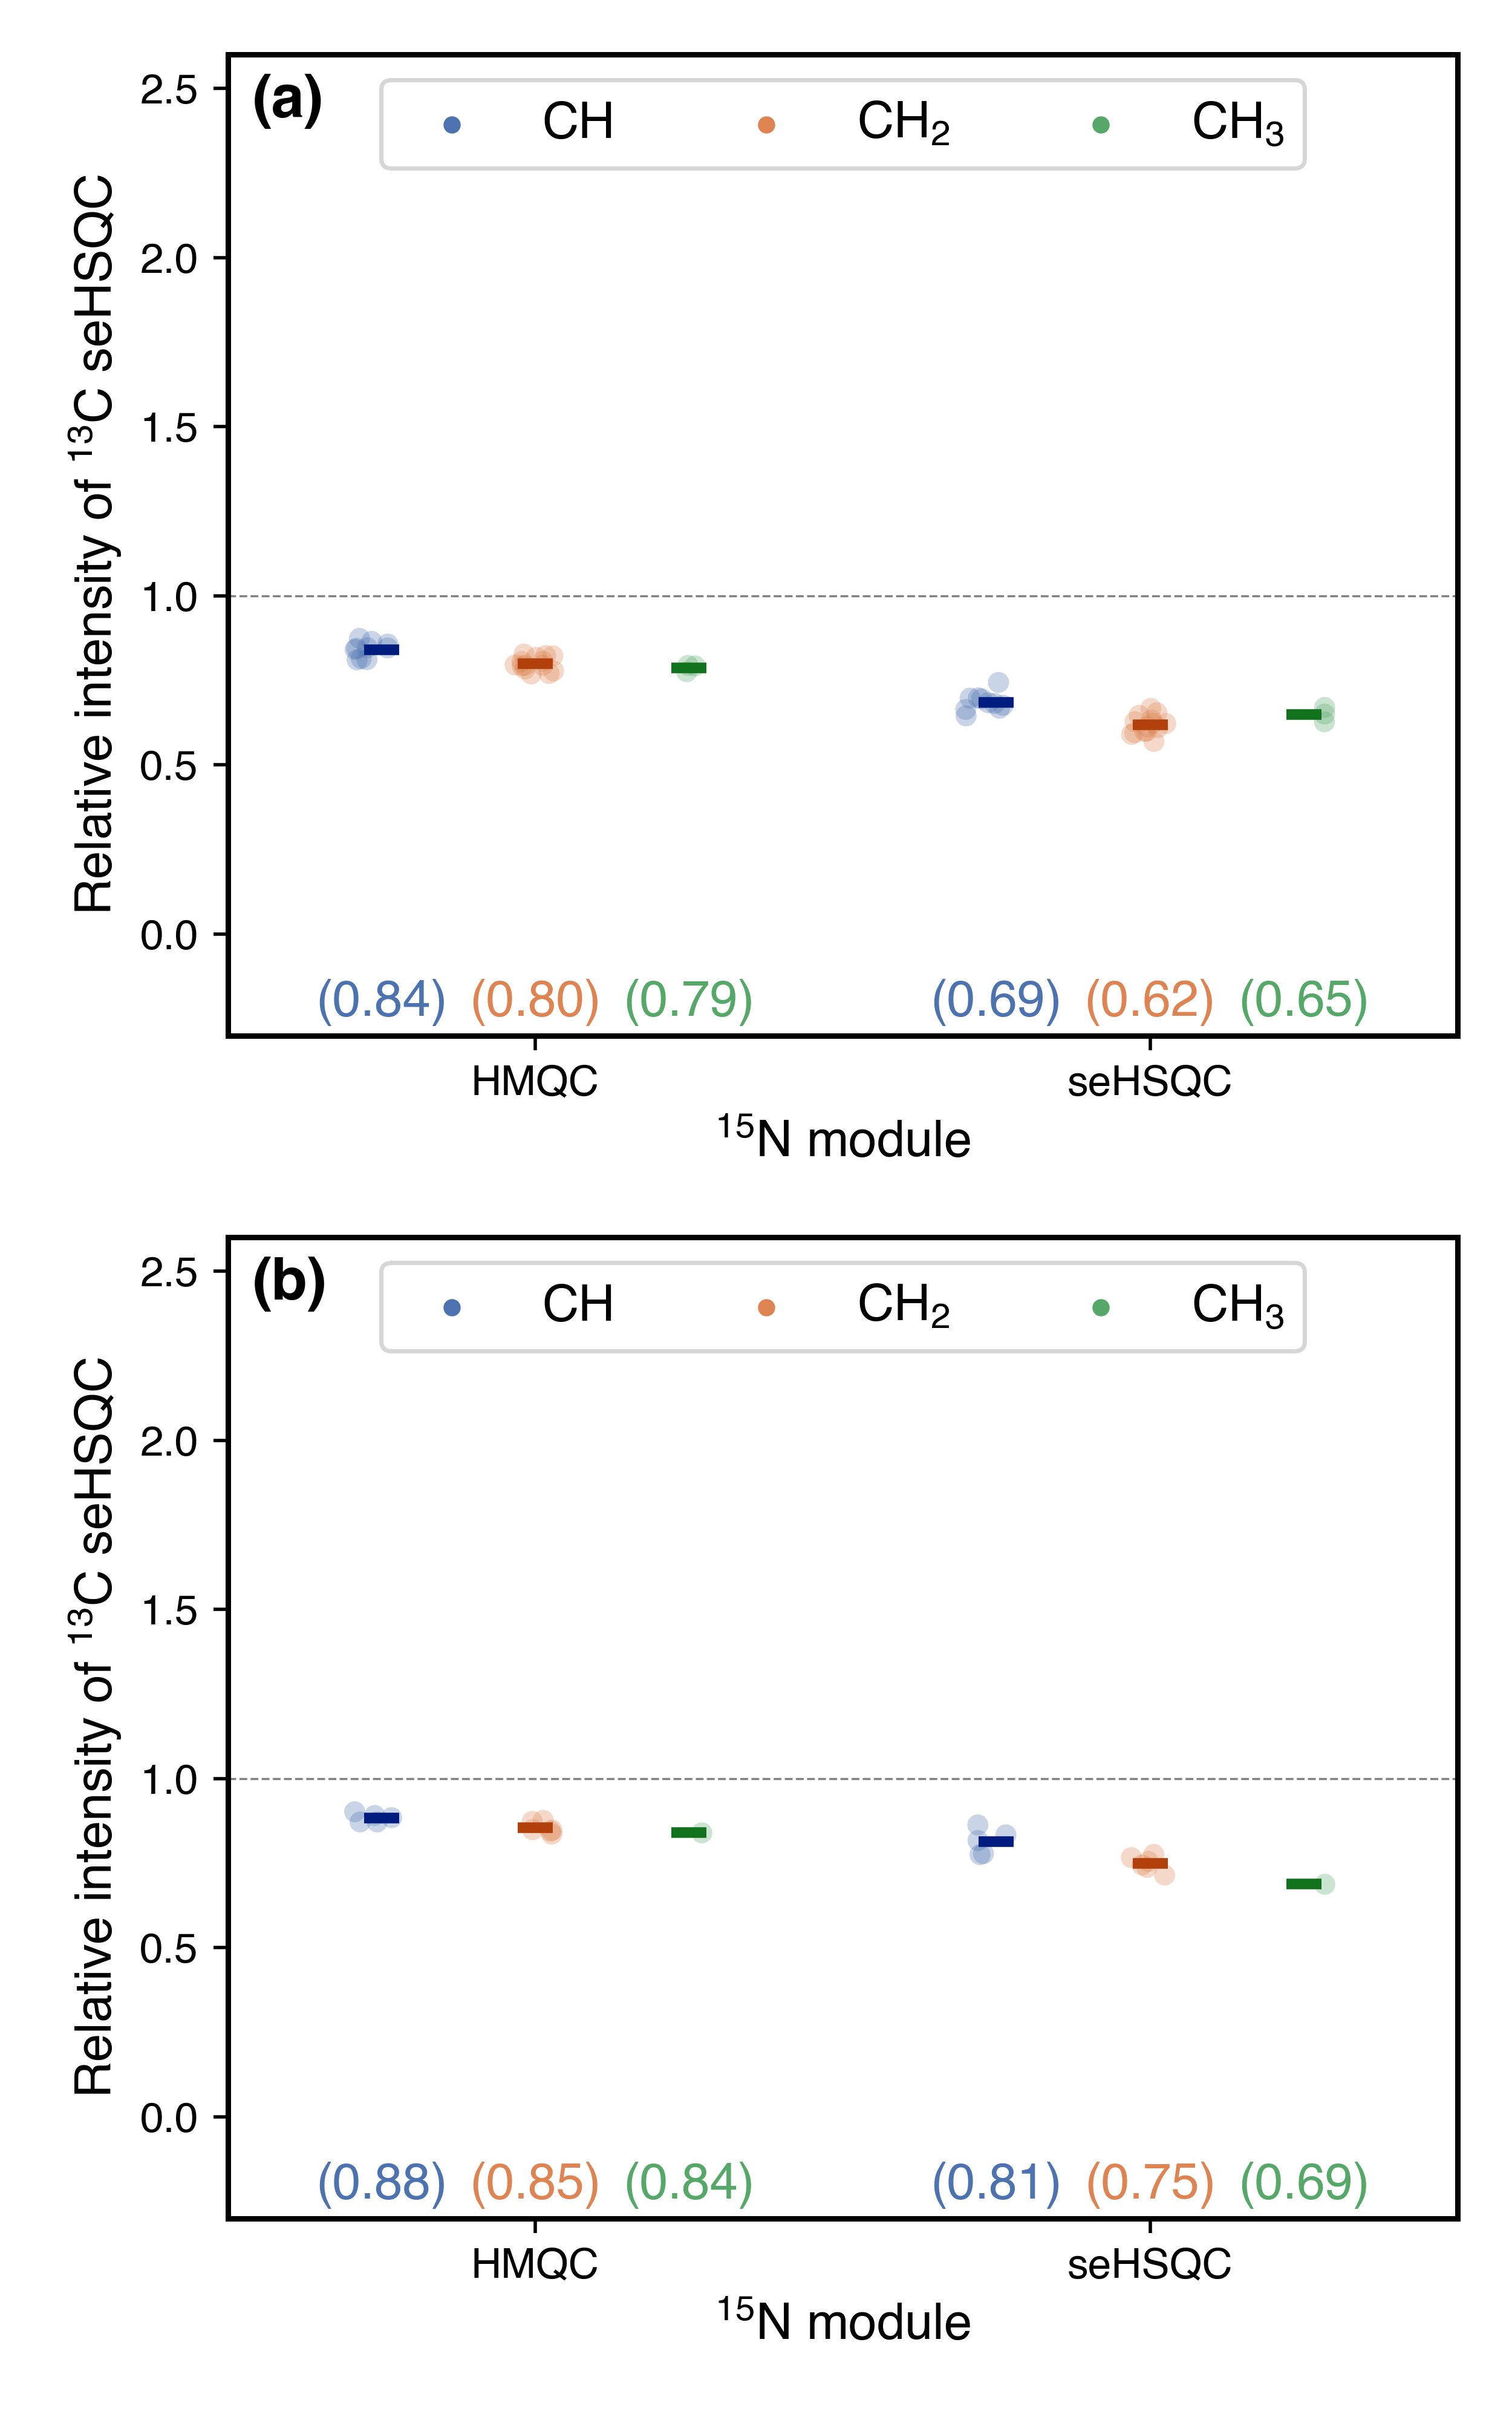
\includegraphics[width=0.9\textwidth]{n15_bulk_retention.png}
    \caption{
        Signal intensities of the \carbon{} seHSQC in NOAH-3 \noahthree{X}{Spb}{Cc} supersequences, normalised against a reference \carbon{} seHSQC taken from a NOAH-2 \noahtwo{Spb}{Cc} supersequence.
        The module \noahX{} is either the \nitrogen{} HMQC (\noahM{}) or the \nitrogen{} seHSQC (\noahSpn{}); the numbers indicate the amount of \magn{\ce{C}} magnetisation that is preserved by the \nitrogen{} module.
        \textbf{(a)} Using \SI{40}{\milli\molar} gramicidin in DMSO-$d_6$.
        \textbf{(b)} Using \SI{50}{\milli\molar} zolmitriptan in DMSO-$d_6$.
        Spectra were obtained on a \SI{700}{\MHz} Bruker AV III equipped with a TCI H/C/N cryoprobe.
    }
    \label{fig:n15_bulk_retention}
\end{figure}


\section{\texorpdfstring{\nitrogen{}}{15N} HSQC and line broadening}

For \proton{}--\nitrogen{} correlations, both the HMQC and version 2 of the new seHSQC are recommended as they keep the bulk magnetisation (both \magn{\ce{C}} and \magnnot{\ce{X}}) along $\pm z$ during the $t_1$ period.
The HSQC module, as well as version 1 of the seHSQC, place this magnetisation in the $xy$-plane during $t_1$, leading to $\jhh$ evolution; consequently, the amount of bulk magnetisation ``passed on'' to the downstream modules decreases as the \nitrogen{} $t_1$ is increased.
Since $t_1$ for each NOAH module is incremented in sync, this is manifested in downstream modules as a $t_1$-dependent decrease in amplitude, or $f_1$ line broadening after Fourier transformation, as shown in \cref{fig:n15_linebroadening}.

\begin{figure}
    \centering
    % figures/n15_linebroadening.py
    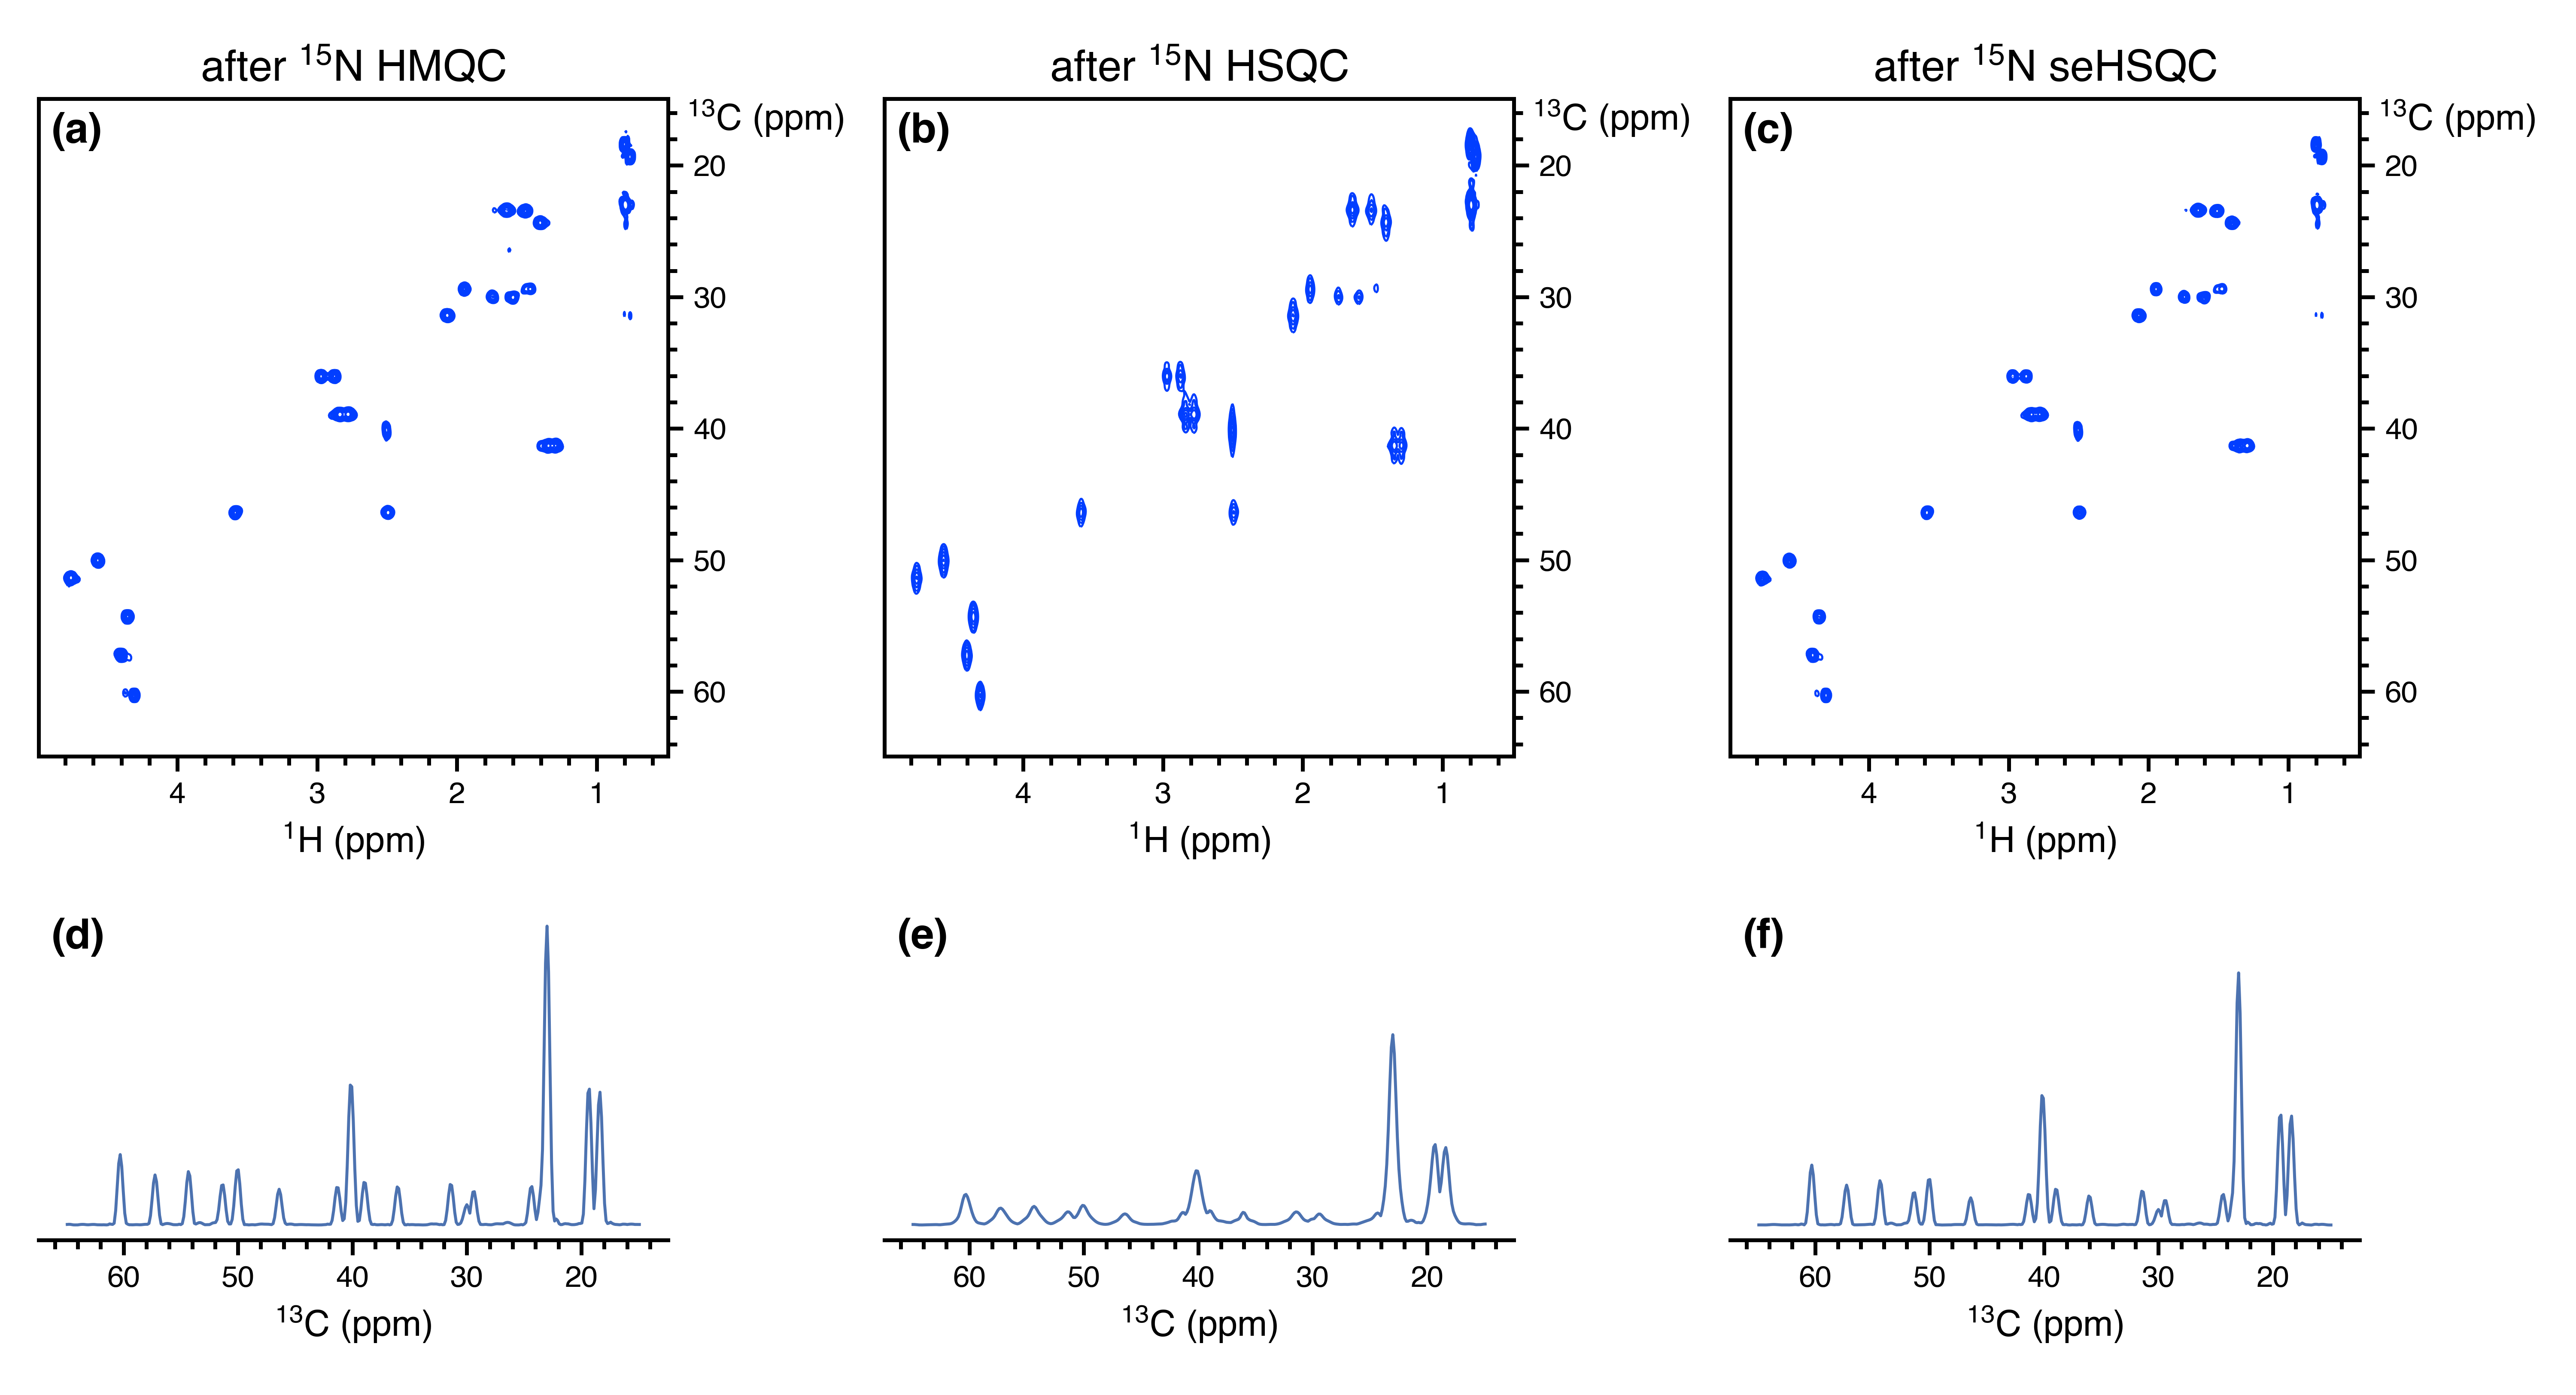
\includegraphics[width=0.9\textwidth]{n15_linebroadening.png}
    {\phantomsubcaption\label{fig:n15_linebroadening_hmqc}}
    {\phantomsubcaption\label{fig:n15_linebroadening_hsqc}}
    {\phantomsubcaption\label{fig:n15_linebroadening_spv2}}
    {\phantomsubcaption\label{fig:n15_linebroadening_hmqc_f2proj}}
    {\phantomsubcaption\label{fig:n15_linebroadening_hsqc_f2proj}}
    {\phantomsubcaption\label{fig:n15_linebroadening_spv2_f2proj}}
    \caption{
        \carbon{} seHSQC spectra obtained from NOAH-3 \noahthree{X}{Spb}{Cc} (\nitrogen{} module + \carbon{} seHSQC + CLIP-COSY) supersequences.
        The \nitrogen{} spectral width was \SI{30}{ppm} and 256 $t_1$ increments were collected, corresponding to an indirect-dimension \nitrogen{} acquisition time of \SI{60.1}{\ms}.
        \textbf{\subref{fig:n15_linebroadening_hmqc}} X = HMQC (``\noahM{}'').
        \textbf{\subref{fig:n15_linebroadening_hsqc}} X = HSQC (``\noahS{}'').
        \textbf{\subref{fig:n15_linebroadening_spv2}} X = seHSQC (``\noahSpn{}'').
        \textbf{\subref{fig:n15_linebroadening_hmqc_f2proj}}--\textbf{\subref{fig:n15_linebroadening_spv2_f2proj}} Projections of spectra \textbf{\subref{fig:n15_linebroadening_hmqc}}--\textbf{\subref{fig:n15_linebroadening_spv2}} onto the $f_1$ axis.
        Note the $f_1$ line broadening in \subref{fig:n15_linebroadening_hsqc} and \subref{fig:n15_linebroadening_hsqc_f2proj}.
        \grami{}
    }
    \label{fig:n15_linebroadening}
\end{figure}

This line broadening also leads to a substantial sensitivity loss (for example, across all peaks, the \carbon{} seHSQC in \cref{fig:n15_linebroadening_hsqc} has almost 65\% lower sensitivity than that in \cref{fig:n15_linebroadening_hmqc}).
The extent of the line broadening depends on the acquisition time (AQ), and is particularly pronounced for long acquisition times, i.e.\ small \nitrogen{} spectral widths.
Thus, the effect may be mitigated by reducing AQ, for example using the scaling methods described in \cref{section:n15_scaling}: indeed, the \SI{60.1}{\ms} used in \cref{fig:n15_linebroadening} to illustrate the effect is often not necessary for \nitrogen{} spectra.
However, even at an AQ of \SI{15.0}{\ms}, there is still discernible broadening which leads to a 25\% loss of sensitivity.
Of course, this issue can be entirely avoided by using either the HMQC or seHSQC.

\section{Effect of lengthened gradients in \texorpdfstring{\nitrogen{}}{15N} modules}
\label{section:n15_cnst16_grads}

\begin{figure}
    \centering
    
\includegraphics[scale=0.9]{zolmi.png}\phantom{aaaaaa}

    % figures/cnst16_diff.py
    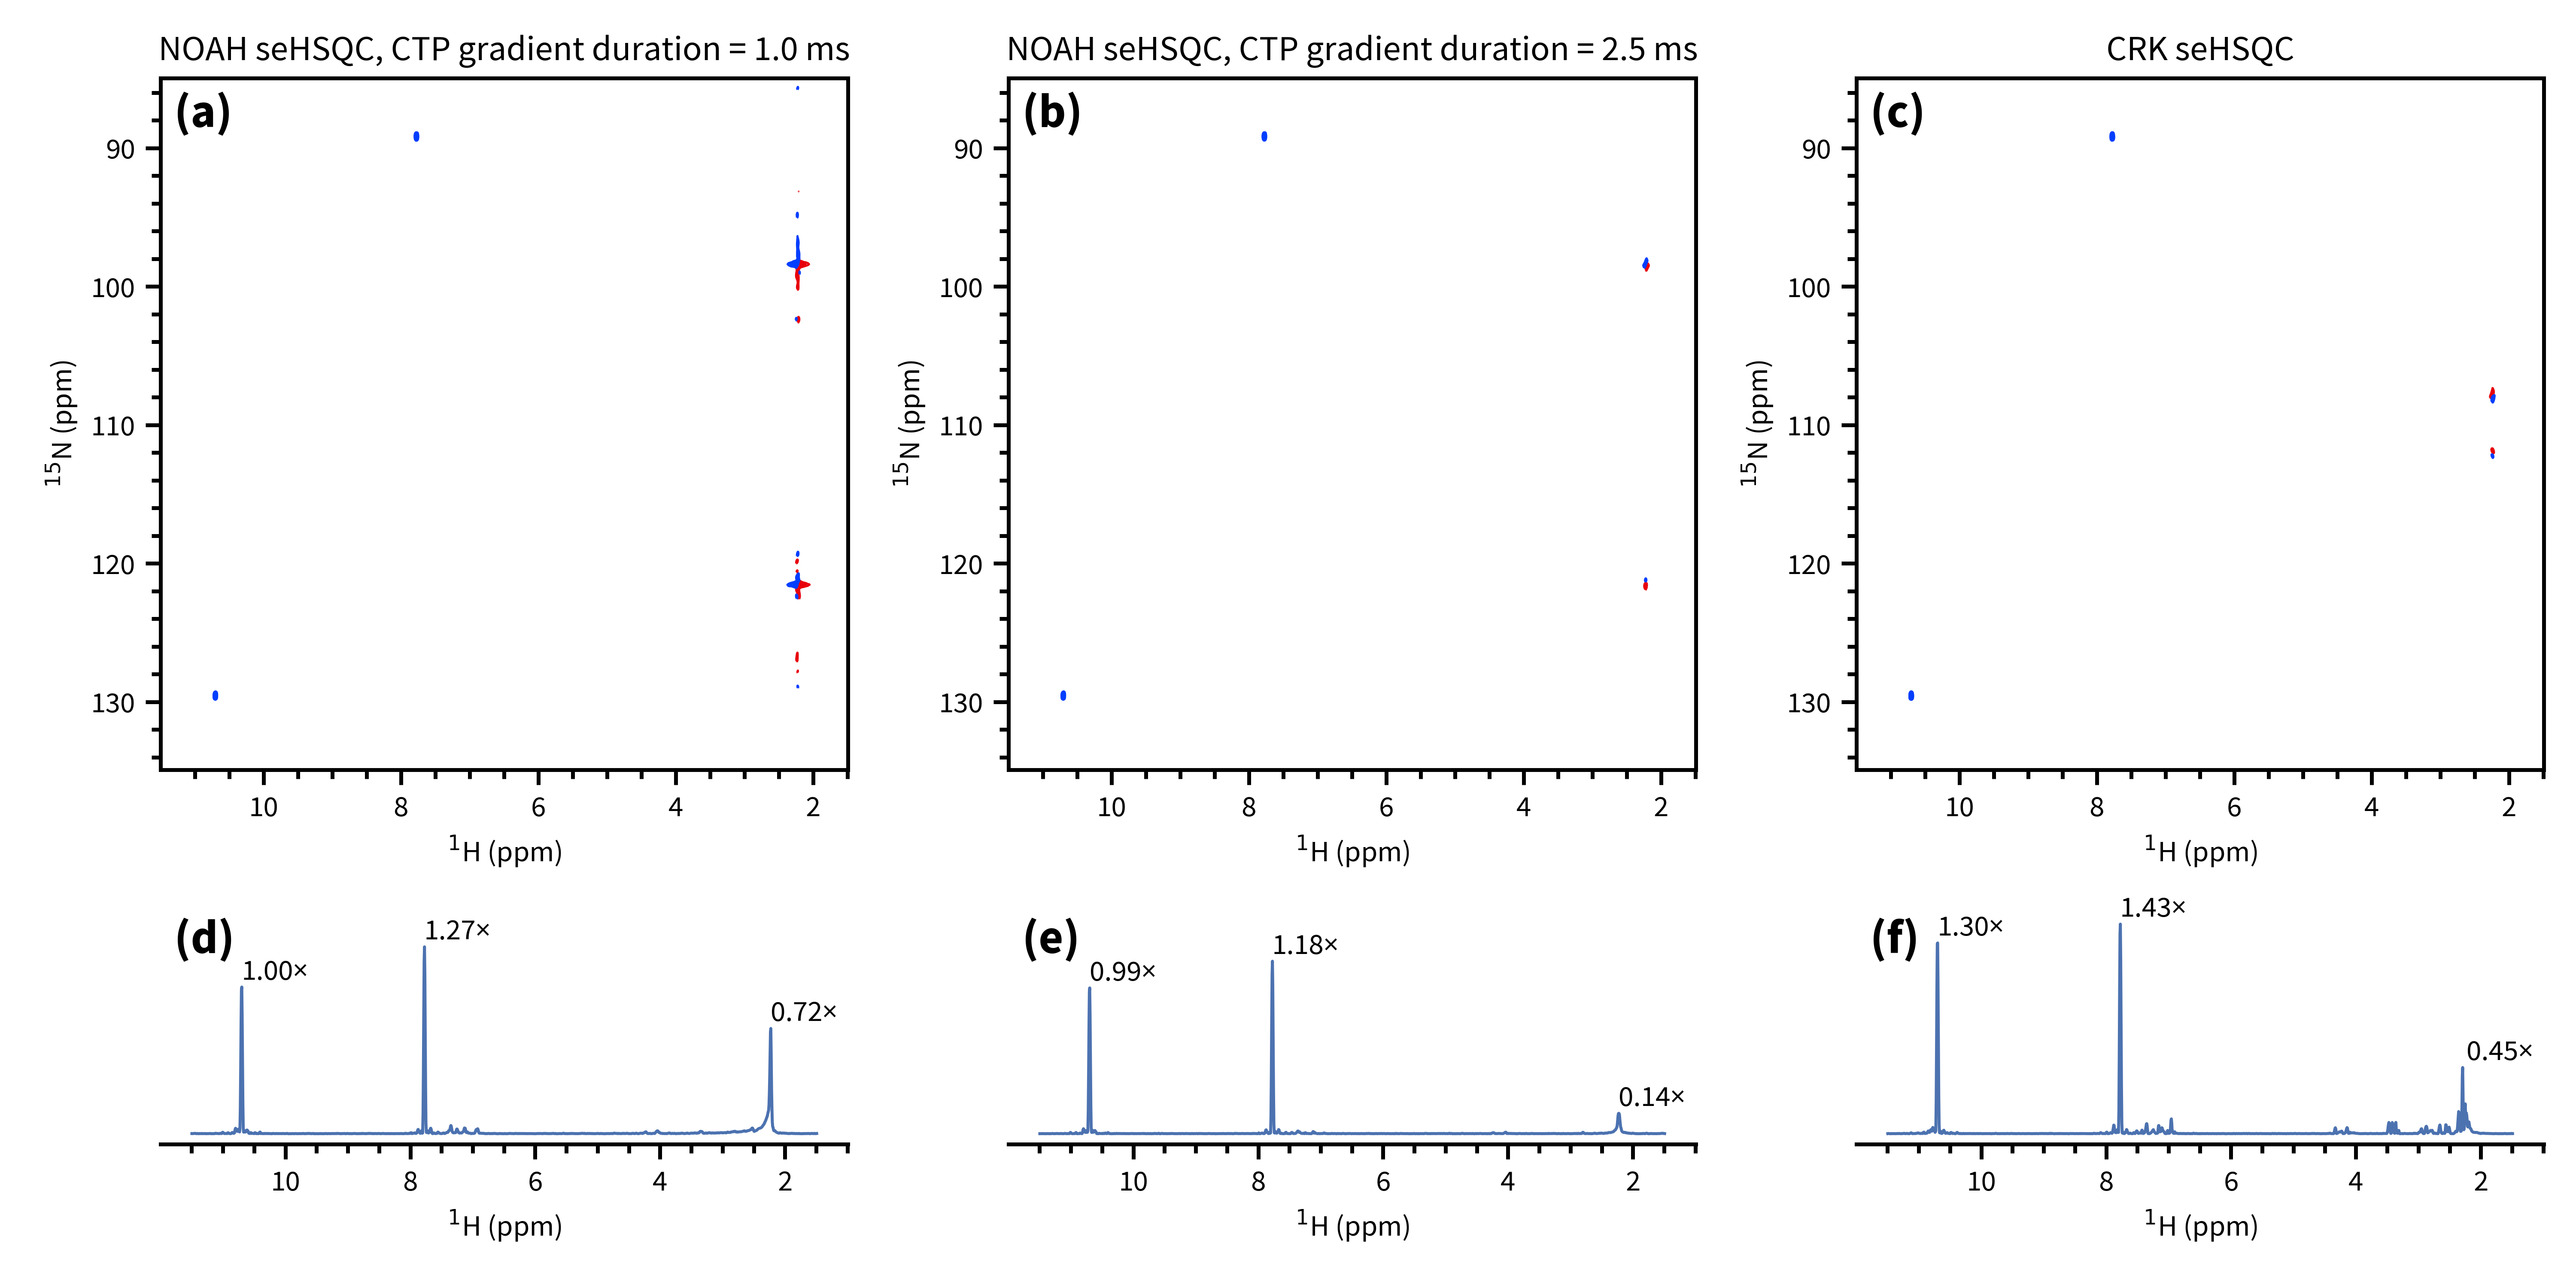
\includegraphics[width=\textwidth]{cnst16_diff.png}
    \caption{
        \nitrogen{} seHSQC spectra obtained using the NOAH and CRK implementations.
        The peaks at 7.8 and \SI{10.7}{\ppm} (\proton{} shifts) are genuine crosspeaks; the mixed-phase peaks at \SI{2.2}{\ppm} are artefacts.
        The 1D \proton{} spectrum is shown above each of the 2D spectra in \textbf{(a)}--\textbf{(c)}; the artefacts seen in the 2D correspond to the intense \textit{N}-methyl groups at \SI{2.2}{\ppm}.
        \textbf{(a)} NOAH seHSQC, with original CTP gradients of \SI{1}{\ms}.
        \textbf{(b)} NOAH seHSQC, with longer CTP gradients of \SI{1}{\ms}.
        \textbf{(c)} Standalone CRK seHSQC with \SI{1}{\ms} CTP gradients (Bruker \texttt{hsqcetf3gpsi2} pulse programme).
        \textbf{(d)}--\textbf{(f)} Projections of spectra \textbf{(a)}--\textbf{(c)} onto the $f_2$ axis.
        The numbers indicate relative peak heights (normalised against the \SI{10.7}{\ppm} peak in (d)).
        \zolmi{}
    }
    \label{fig:cnst16_diff}
\end{figure}

The lengthening of CTP gradients from \SI{1}{\ms} to \SI{2.5}{\ms} is aimed at cleaning up artefacts arising from bulk magnetisation that is not properly returned to $+z$ at the end of the sequence.
\cref{fig:cnst16_diff} shows exactly how effective this strategy is.
In (d), where the CTP gradients have their original duration, the artefacts originating from the intense methyl groups have comparable intensity to the desired peaks.
When the gradients are lengthened in (e), the crosspeak intensities are almost unaffected, whereas the artefacts are suppressed by a factor of 5 or more.
Although this suppression is not complete, this should not be interpreted as a weakness of the new NOAH seHSQC module, as similar artefacts are also visible in the CRK seHSQC (f).
Indeed, every \proton{}--\nitrogen{} experiment we tested has at least \textit{some} artefact intensity in this region.

\section{Sensitivity and resolution in \texorpdfstring{\nitrogen{}}{15N} modules}
\label{section:n15_scaling}

\subsection{Overview}

In ideal cases, it is possible to modify the acquisition scheme of a 2D experiment, such that resolution in the indirect dimension is decreased in return for gains in sensitivity: this has previously been illustrated in the context of time-shared \nitrogen{},\carbon{} HMBC spectra.\autocite{Perez-Trujillo2007MRC,Parella2010CMR}
This can prove to be useful particularly in \nitrogen{} modules, where the number of peaks is typically small, and are well-dispersed across the chemical shift range (thus minimising the chances of accidental overlap).
The key parameter here is the indirect-dimension acquisition time (AQ): a shorter AQ leads to poorer resolution but higher sensitivity (ideally).
We propose two different, but ultimately very similar, methods of reducing AQ:

\begin{enumerate}
    \item $k$-scaling: decreasing the number of $t_1$ increments (TD1) by a factor of $k$ leads to a decrease in AQ by a factor of $k$. In its place, the number of scans (NS) can be increased by a factor of $k$.
    \item SW-scaling: increasing the indirect-dimension spectral width (SW) by a factor of $k$ (but leaving TD1 and NS unchanged) leads to an equivalent decrease in AQ.
\end{enumerate}

These possibilities are illustrated schematically in \cref{fig:kscale_overview}.
The ``standard'' experiment (\cref{fig:kscale_overview_std}) is acquired as described in the \textit{Experimental} section of the main text, i.e.\ TD1 = 256, NS = 2, and SW = 30 ppm (for gramicidin).

\subsection{Standard processing as performed in this work}

For both the $k$- and SW-scaled spectra, the entries that are \textit{not} marked ``(+LP)'' are processed as described in the \textit{Experimental} section of the main text.
In particular, linear prediction is used to construct another TD1 points beyond the TD1 originally acquired points, which corresponds to setting the processing parameters ME\_mod = `LPfc' (or `LPfr') and LPbin = 0.
This leads to an \textit{effective acquisition time}, $\aqeff$, which is double the original acquisition time AQ: in practice, the indirect-dimension resolution is not determined by AQ but rather $\aqeff$.

The results of $k$- and SW-scaling are illustrated in \cref{fig:hmqc_kscale,fig:spv2_kscale} for \nitrogen{} HMQC and seHSQC spectra respectively.
By decreasing the indirect dimension resolution, the $f_1$ linewidths of the peaks increase: this can lead to significant sensitivity enhancement for the HMQC (up to $2.6 \times$), because $\jhh$ splitting in the $f_1$ dimension is no longer resolved.
The largest gains are observed for peaks where $\jhh$ splitting is better resolved; for the leftmost peak at $\delta_{\ce{N}} = \SI{128}{\ppm}$ which has no resolved $\jhh$ splitting, only a more modest $1.7 \times$ gain in sensitivity is attained.
For the seHSQC module, $k$-scaling on its own leads to far smaller sensitivity gains (\cref{fig:spv2_kscale}).
Any increase in the total peak volume is almost completely offset by the $f_1$ broadening.
Therefore, even at $k = 8$, the largest sensitivity gains that can be attained are $\sim 1.3\times$.

\subsection{Extra linear prediction}

It is clear, however, that $\aqeff$ can be arbitrarily extended by applying more extensive linear prediction: this is the case for the experiments in \cref{fig:kscale_overview_std} marked with ``(+LP)''.
In each case, we have applied linear prediction up to the original $\aqeff$ of \SI{120.3}{\ms} in order to recover the resolution of the ``standard'' spectrum.
Although this leads to larger increases in peak height or SNR (by virtue of the decreased linewidths), this does not necessarily represent a true ``sensitivity gain'' in terms of the ability to reveal weak peaks.\autocite{snrsens}

Aggressive linear prediction is less successful for the HMQC spectra (\cref{fig:hmqc_kscale_lp}): although raw gains in peak height can be observed for all values of $k$, there is a corresponding decrease in the spectral quality, as evidenced by the $f_1$ multiplet structure becoming increasingly distorted.
On the other hand, linear prediction performs well for the seHSQC spectra (\cref{fig:spv2_kscale_lp}), where there is no multiplet structure in $f_1$.


\subsection{Discussion}

It is difficult to draw firm conclusions from the spectra shown here, but some general guidelines may be mentioned:

\begin{itemize}
    \item The sensitivity gains obtained without extra linear prediction (\cref{fig:hmqc_kscale,fig:spv2_kscale}) are almost identical for both $k$- and SW-scaling.
    \item $k$-scaling appears to provide larger raw gains in peak height when extra linear prediction is applied (\cref{fig:hmqc_kscale_lp,fig:spv2_kscale_lp}), although the fidelity of the reconstruction at large values of $k$ is questionable, particularly for the HMQC.
    \item $k$-scaling is currently not compatible with the use of non-uniform sampling (NUS) in the rest of the NOAH supersequence, because two distinct NUS schedules would have to be maintained in the pulse programme (one for the $k$-scaled module and one for the other modules).
        If NUS is desired, then SW-scaling is the only viable option.
\end{itemize}

It should also be noted that $k$-scaling is a special case of \textit{undersampling}, where the sampling schedule is chosen to simply be the first $\mathrm{TD1}/k$ points, and the remainder reconstructed via linear prediction.
A possible alternative would be to choose a different (non-uniform) sampling schedule for the \nitrogen{} module to reduce the number of $t_1$ increments, and in turn increase NS; the missing increments may be reconstructed using a number of NUS algorithms.
We briefly investigated this on the present sample, but did not see any noticeable differences as compared to $k$-scaling.
However, it is possible that under different circumstances, \textit{bona fide} sensitivity gains may be attained compared to the ``standard'' spectrum.\autocite{Mobli2014PNMRS,Palmer2015JPCB}


\begin{figure}
    \centering
    % Inkscape
    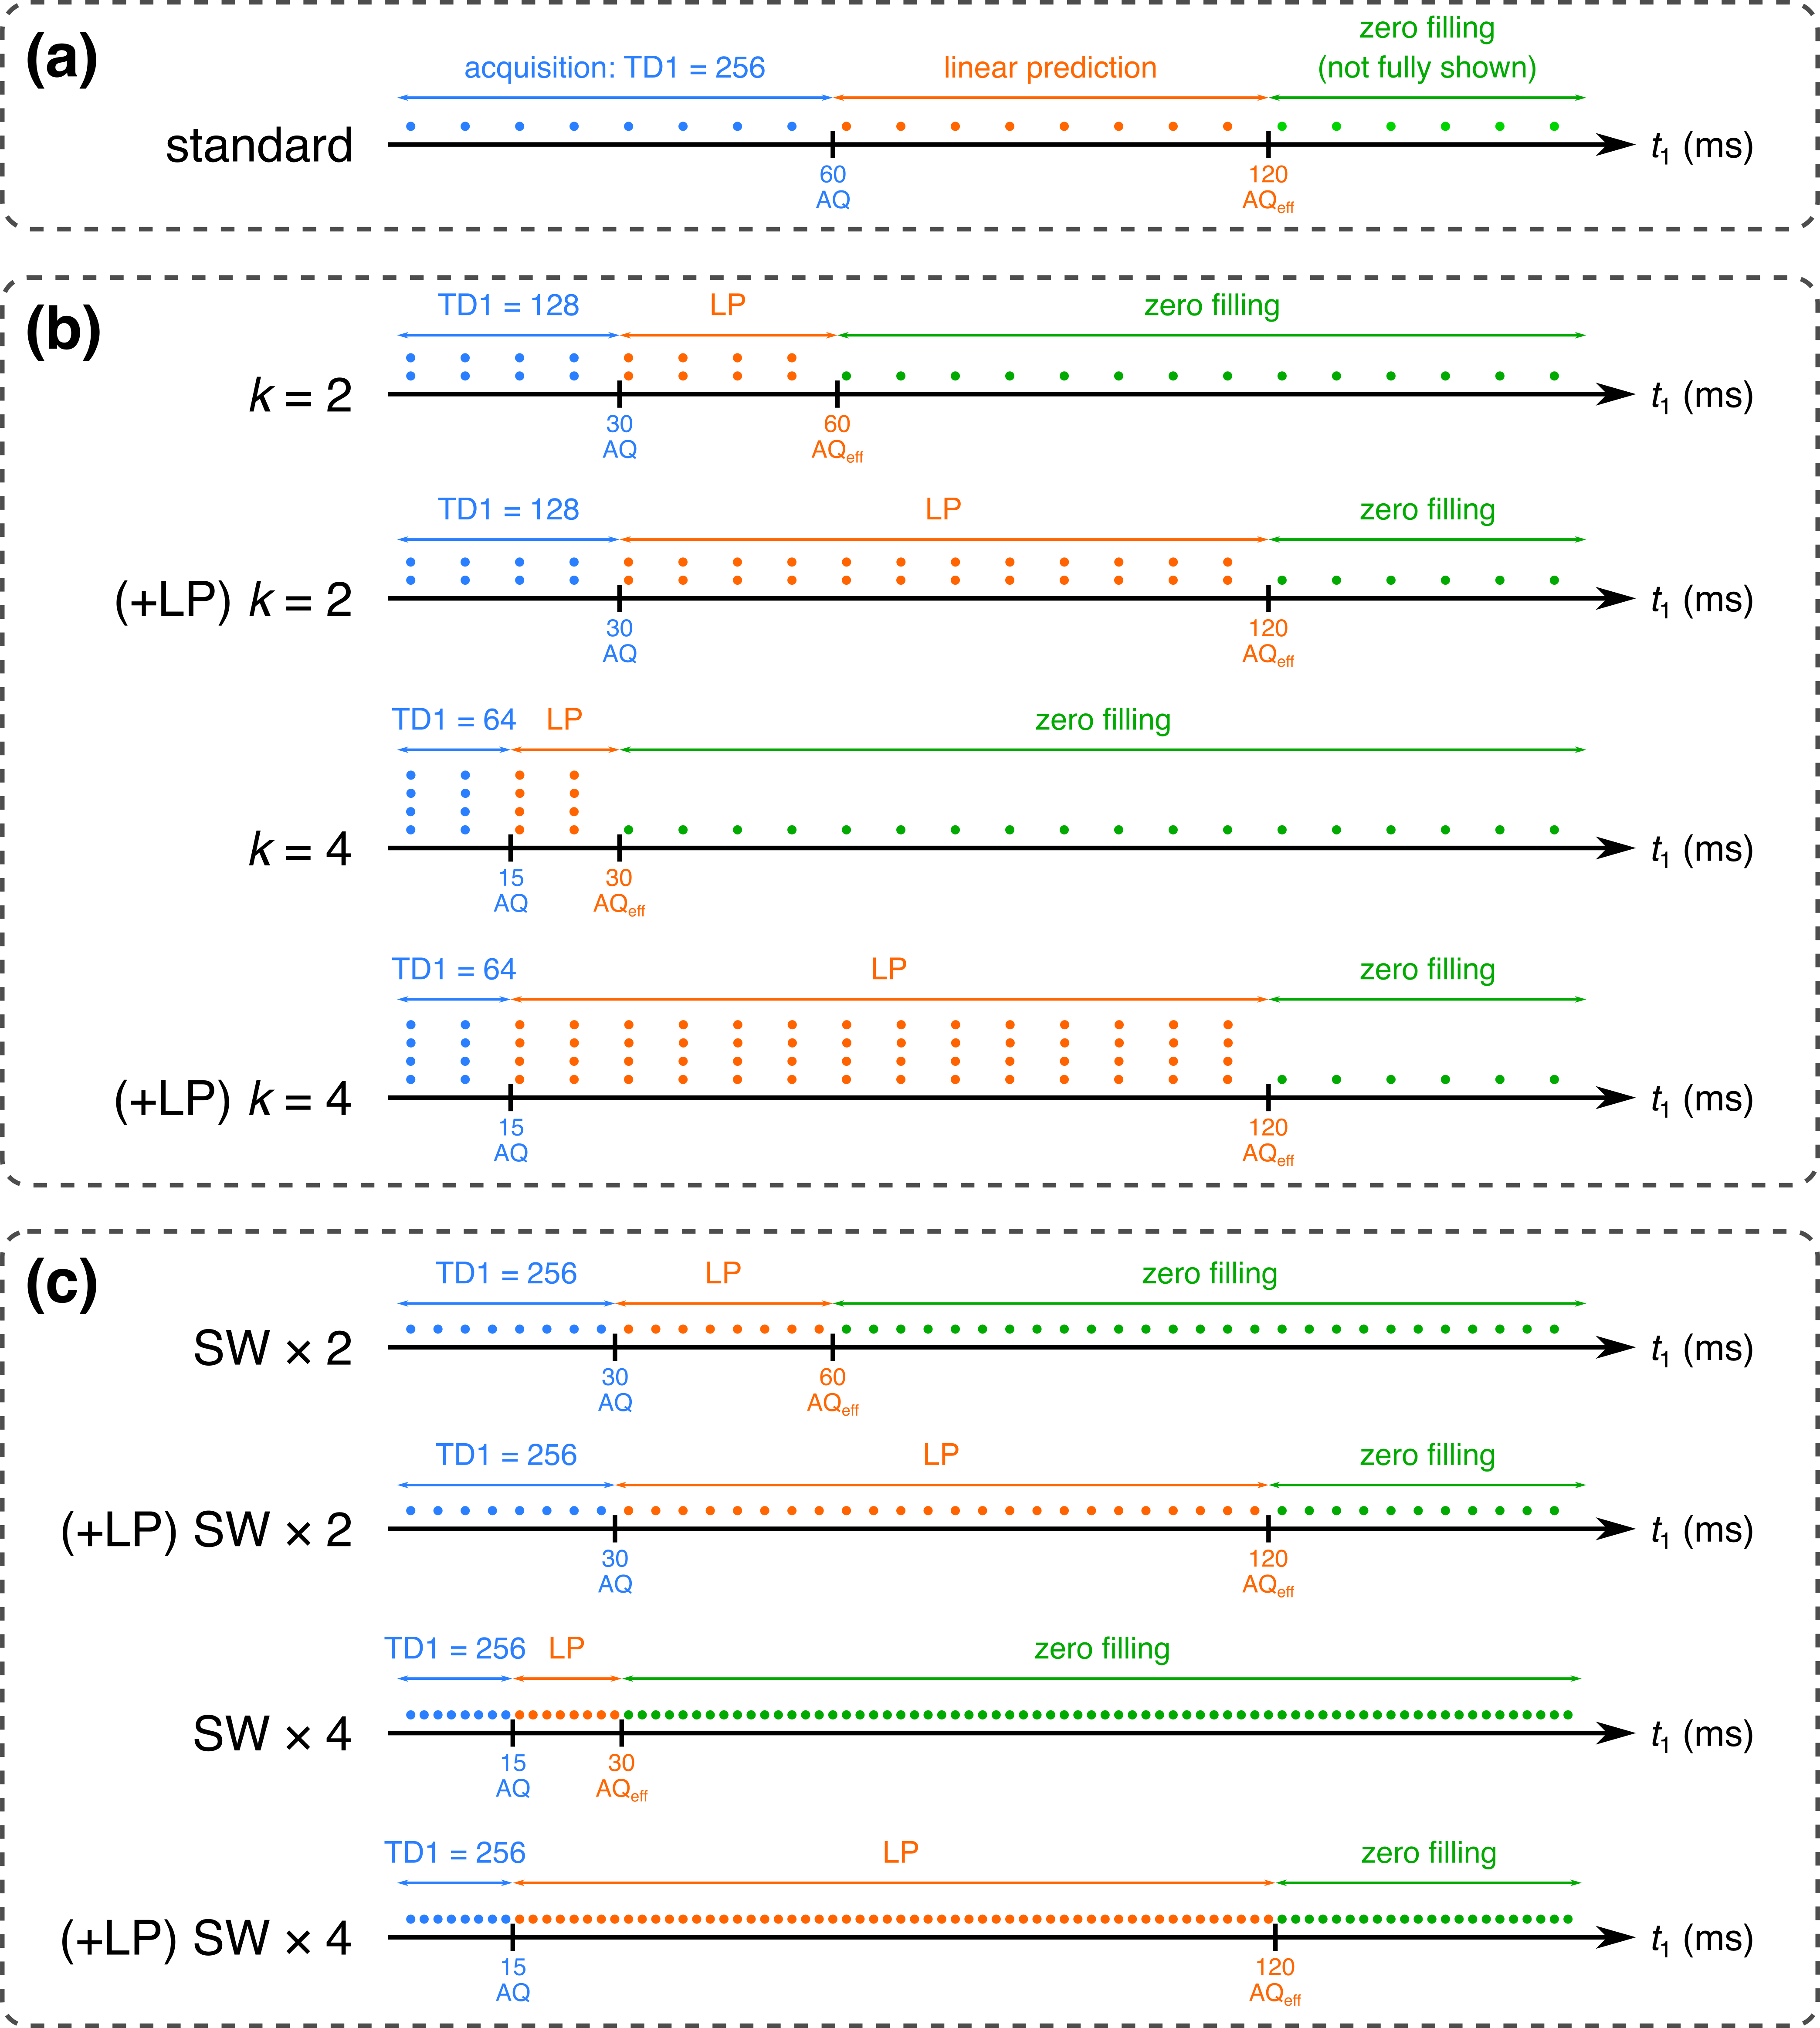
\includegraphics[width=0.8\textwidth]{kscale_overview.png}
    {\phantomsubcaption\label{fig:kscale_overview_std}}
    {\phantomsubcaption\label{fig:kscale_overview_k}}
    {\phantomsubcaption\label{fig:kscale_overview_sw}}
    \caption{
        Pictorial representation of $k$- and SW-scaling, the two ways of reducing the indirect-dimension AQ discussed in the text.
        Each dot represents 32 $t_1$ increments with 2 scans per increment: blue dots indicate physically acquired data, orange dots indicate data constructed via forward linear prediction, and green dots indicate zeroes used to pad the FID in zero filling (not all zeroes are shown here).
        The total experimental time is proportional to the number of blue dots, and is kept constant in all of the above; the SNR is to a first approximation proportional to the square root of the number of blue and orange dots.
        The true indirect-dimension acquisition time (AQ), as well as an ``effective'' acquisition time obtained through linear prediction ($\aqeff$), are indicated on the $t_1$ axis.
        The observed indirect-dimension resolution is directly proportional to $\aqeff$.
        In all experiments not marked ``(+LP)'', linear prediction is performed such that $\aqeff = 2 \times \mathrm{AQ}$.
        Experiments marked ``(+LP)'' have \textit{extra} linear prediction applied in order to extend $\aqeff$ to the original value of $\SI{120.3}{\ms}$.
        \textbf{\subref{fig:kscale_overview_std}} The ``standard'' experiment.
        \textbf{\subref{fig:kscale_overview_k}} $k$-scaled experiments, where the number of $t_1$ increments (TD1) is reduced in favour of an increased number of scans (NS) per increment (symbolised by the vertically stacked dots).
        \textbf{\subref{fig:kscale_overview_sw}} SW-scaled experiments, where TD1 and NS remain unchanged, but the spacing between increments is decreased.
        Notice how AQ and $\aqeff$ are modified in exactly the same way as in \subref{fig:kscale_overview_k}.
        The effects of $k$- and SW-scaling are compared in \cref{fig:hmqc_kscale,fig:spv2_kscale,fig:hmqc_kscale_lp,fig:spv2_kscale_lp}.
    }
    \label{fig:kscale_overview}
\end{figure}

\begin{figure}
    \centering
    % figures/hmqc_kscale.py
    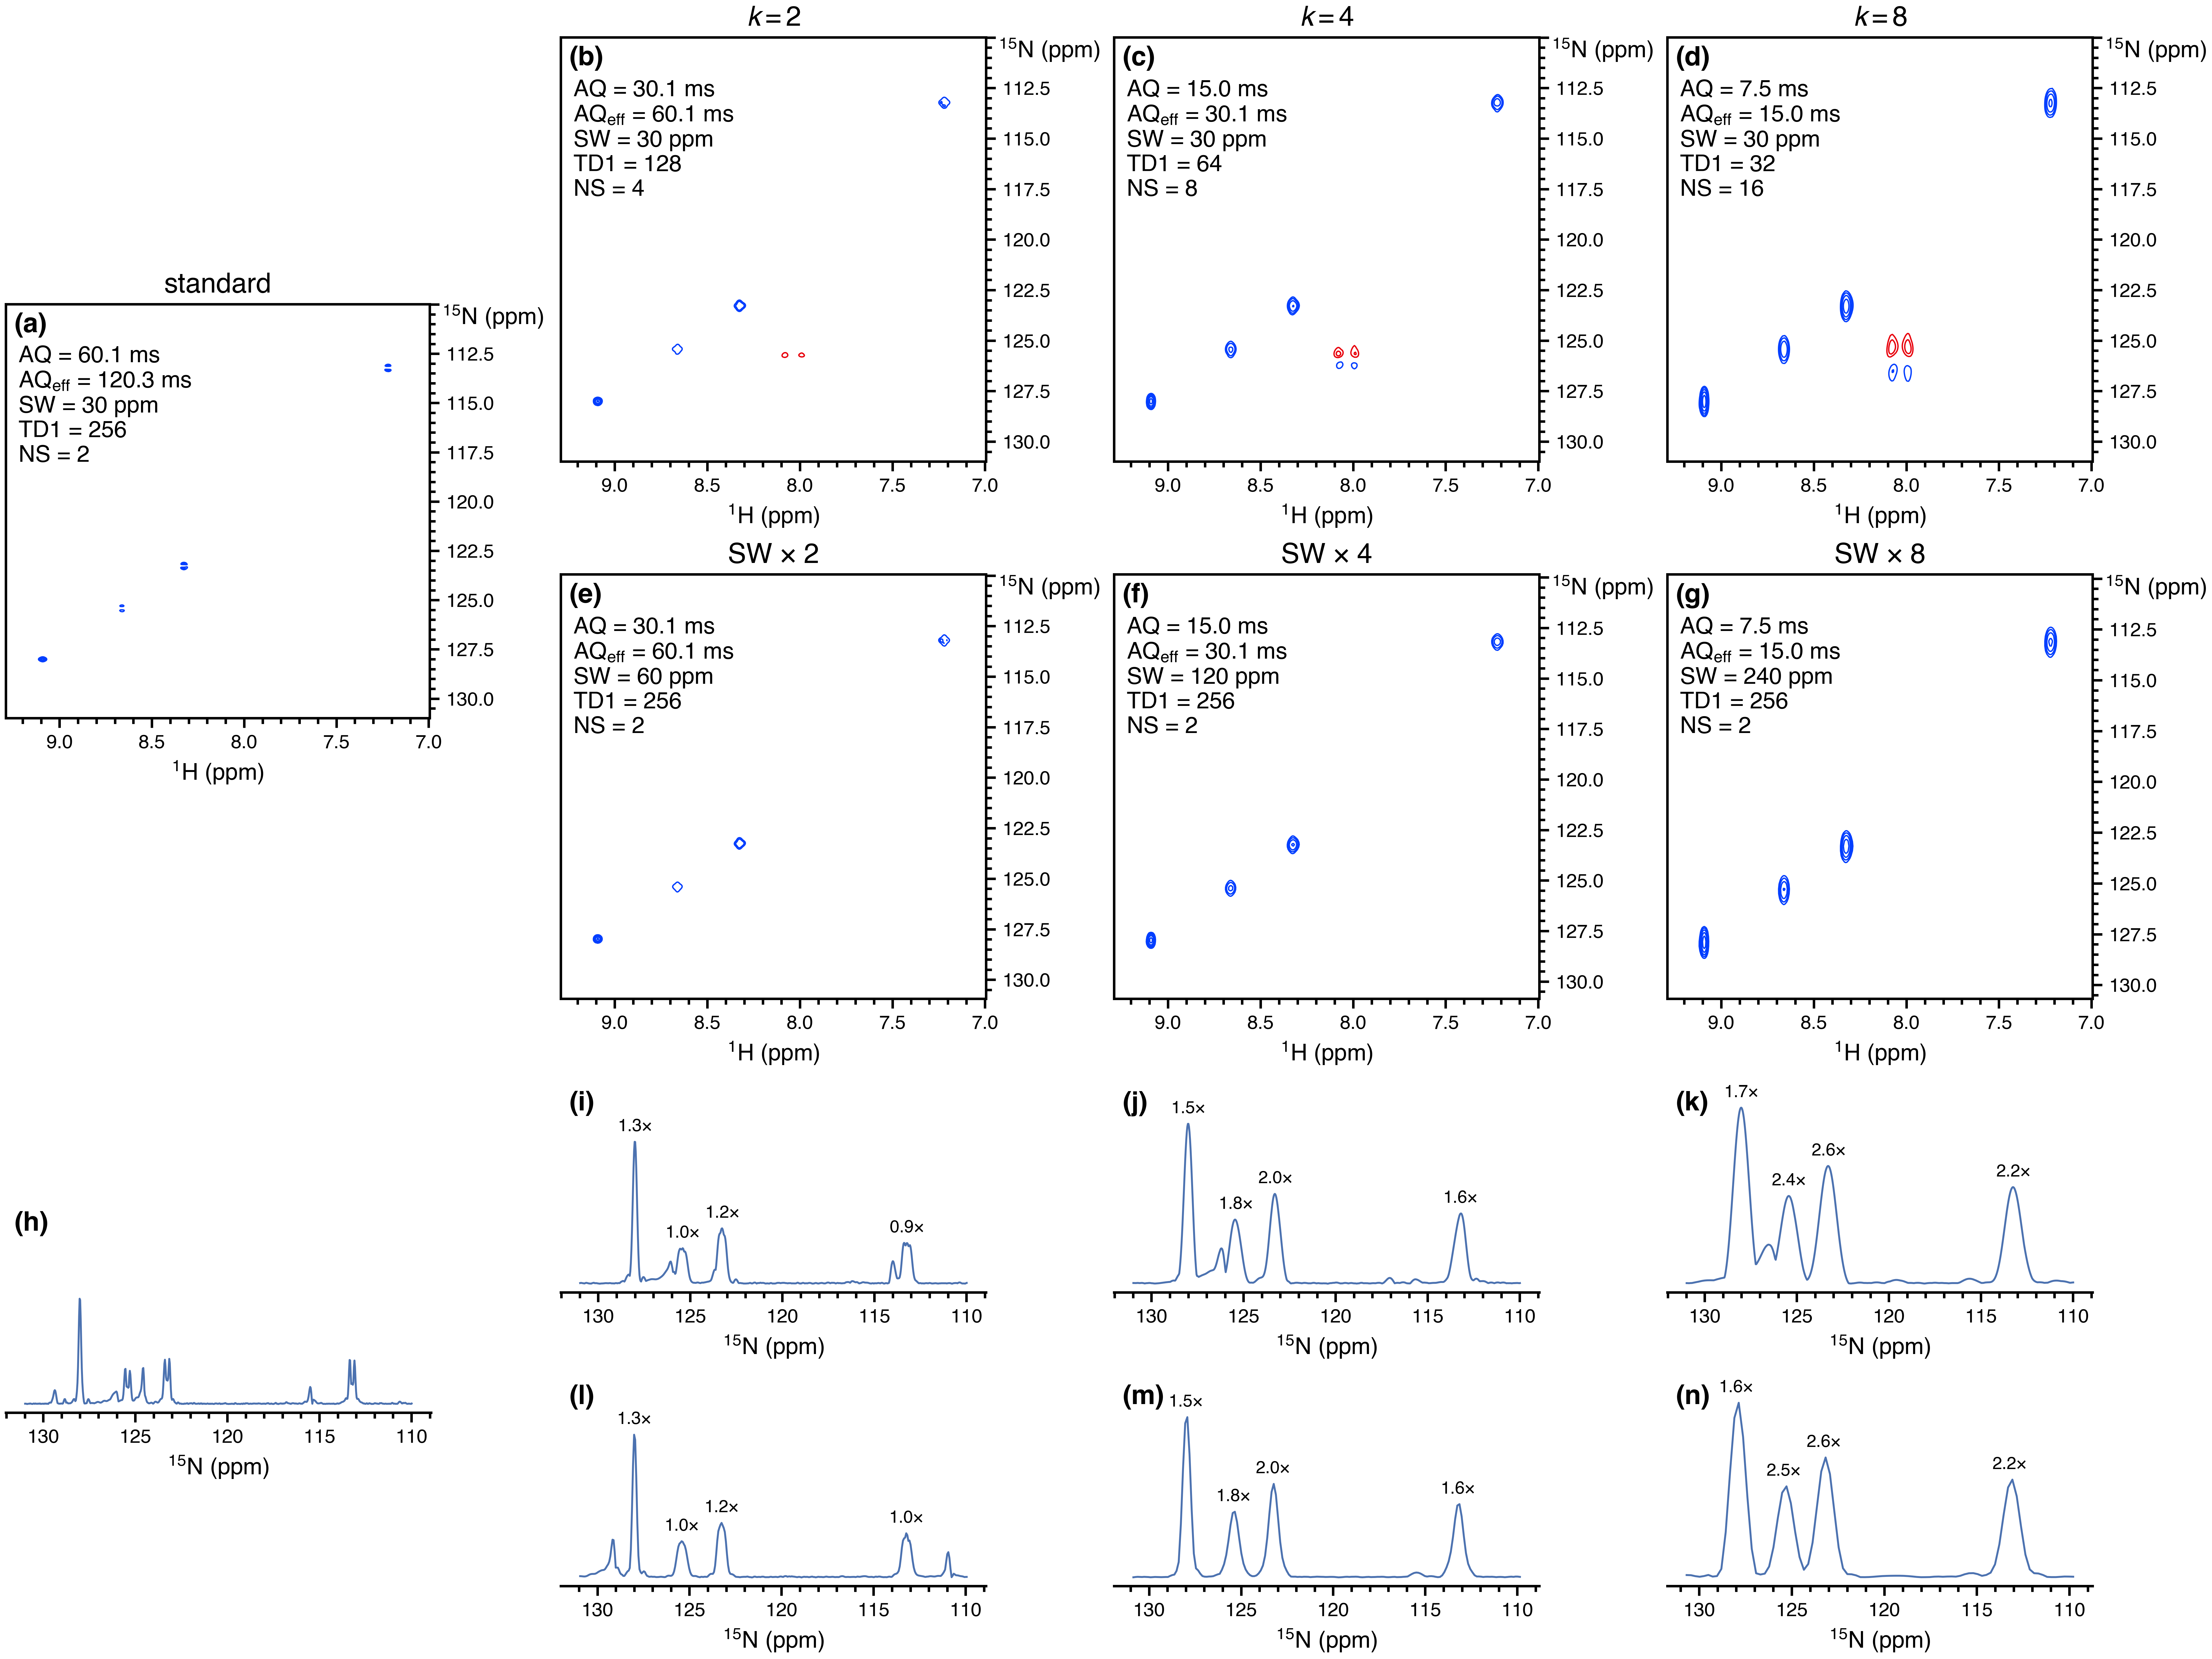
\includegraphics[width=\textwidth]{hmqc_kscale.png}
    {\phantomsubcaption\label{fig:hmqc_kscale_std}}
    {\phantomsubcaption\label{fig:hmqc_kscale_k2}}
    {\phantomsubcaption\label{fig:hmqc_kscale_k4}}
    {\phantomsubcaption\label{fig:hmqc_kscale_k8}}
    {\phantomsubcaption\label{fig:hmqc_kscale_sw2}}
    {\phantomsubcaption\label{fig:hmqc_kscale_sw4}}
    {\phantomsubcaption\label{fig:hmqc_kscale_sw8}}
    {\phantomsubcaption\label{fig:hmqc_kscale_std_proj}}
    {\phantomsubcaption\label{fig:hmqc_kscale_k2_proj}}
    {\phantomsubcaption\label{fig:hmqc_kscale_k4_proj}}
    {\phantomsubcaption\label{fig:hmqc_kscale_k8_proj}}
    {\phantomsubcaption\label{fig:hmqc_kscale_sw2_proj}}
    {\phantomsubcaption\label{fig:hmqc_kscale_sw4_proj}}
    {\phantomsubcaption\label{fig:hmqc_kscale_sw8_proj}}
    \caption{
        \textbf{(HMQC without extra linear prediction.)}
        \nitrogen{} HMQC spectra taken from NOAH-3 \noahthree{M}{Spb}{Cc} supersequences.
        All spectra are plotted with the same noise levels.
        No linear prediction has been applied beyond the standard processing; thus, $\aqeff$ is equal to $2 \times \mathrm{AQ}$ for all of the spectra above.
        \textbf{\subref{fig:hmqc_kscale_std}} The ``standard'' spectrum.
        \textbf{\subref{fig:hmqc_kscale_k2}} $k = 2$.
        \textbf{\subref{fig:hmqc_kscale_k4}} $k = 4$.
        \textbf{\subref{fig:hmqc_kscale_k8}} $k = 8$.
        \textbf{\subref{fig:hmqc_kscale_sw2}} $\mathrm{SW} \times 2$.
        \textbf{\subref{fig:hmqc_kscale_sw4}} $\mathrm{SW} \times 4$.
        \textbf{\subref{fig:hmqc_kscale_sw8}} $\mathrm{SW} \times 8$.
        \textbf{\subref{fig:hmqc_kscale_std_proj}}--\textbf{\subref{fig:hmqc_kscale_sw8_proj}} Projections of 2D spectra in \subref{fig:hmqc_kscale_std}--\subref{fig:hmqc_kscale_sw8} onto the $f_1$ axis.
        Numbers indicate peak heights relative to the ``standard'' HMQC spectrum in \subref{fig:hmqc_kscale_std}.
        The peak at $\delta_{\ce{H}} = \SI{8.03}{\ppm}$ is folded and therefore does not appear in the SW-scaled spectra.
        \grami{}
    }
    \label{fig:hmqc_kscale}
\end{figure}

\begin{figure}
    \centering
    % figures/spv2_kscale.py
    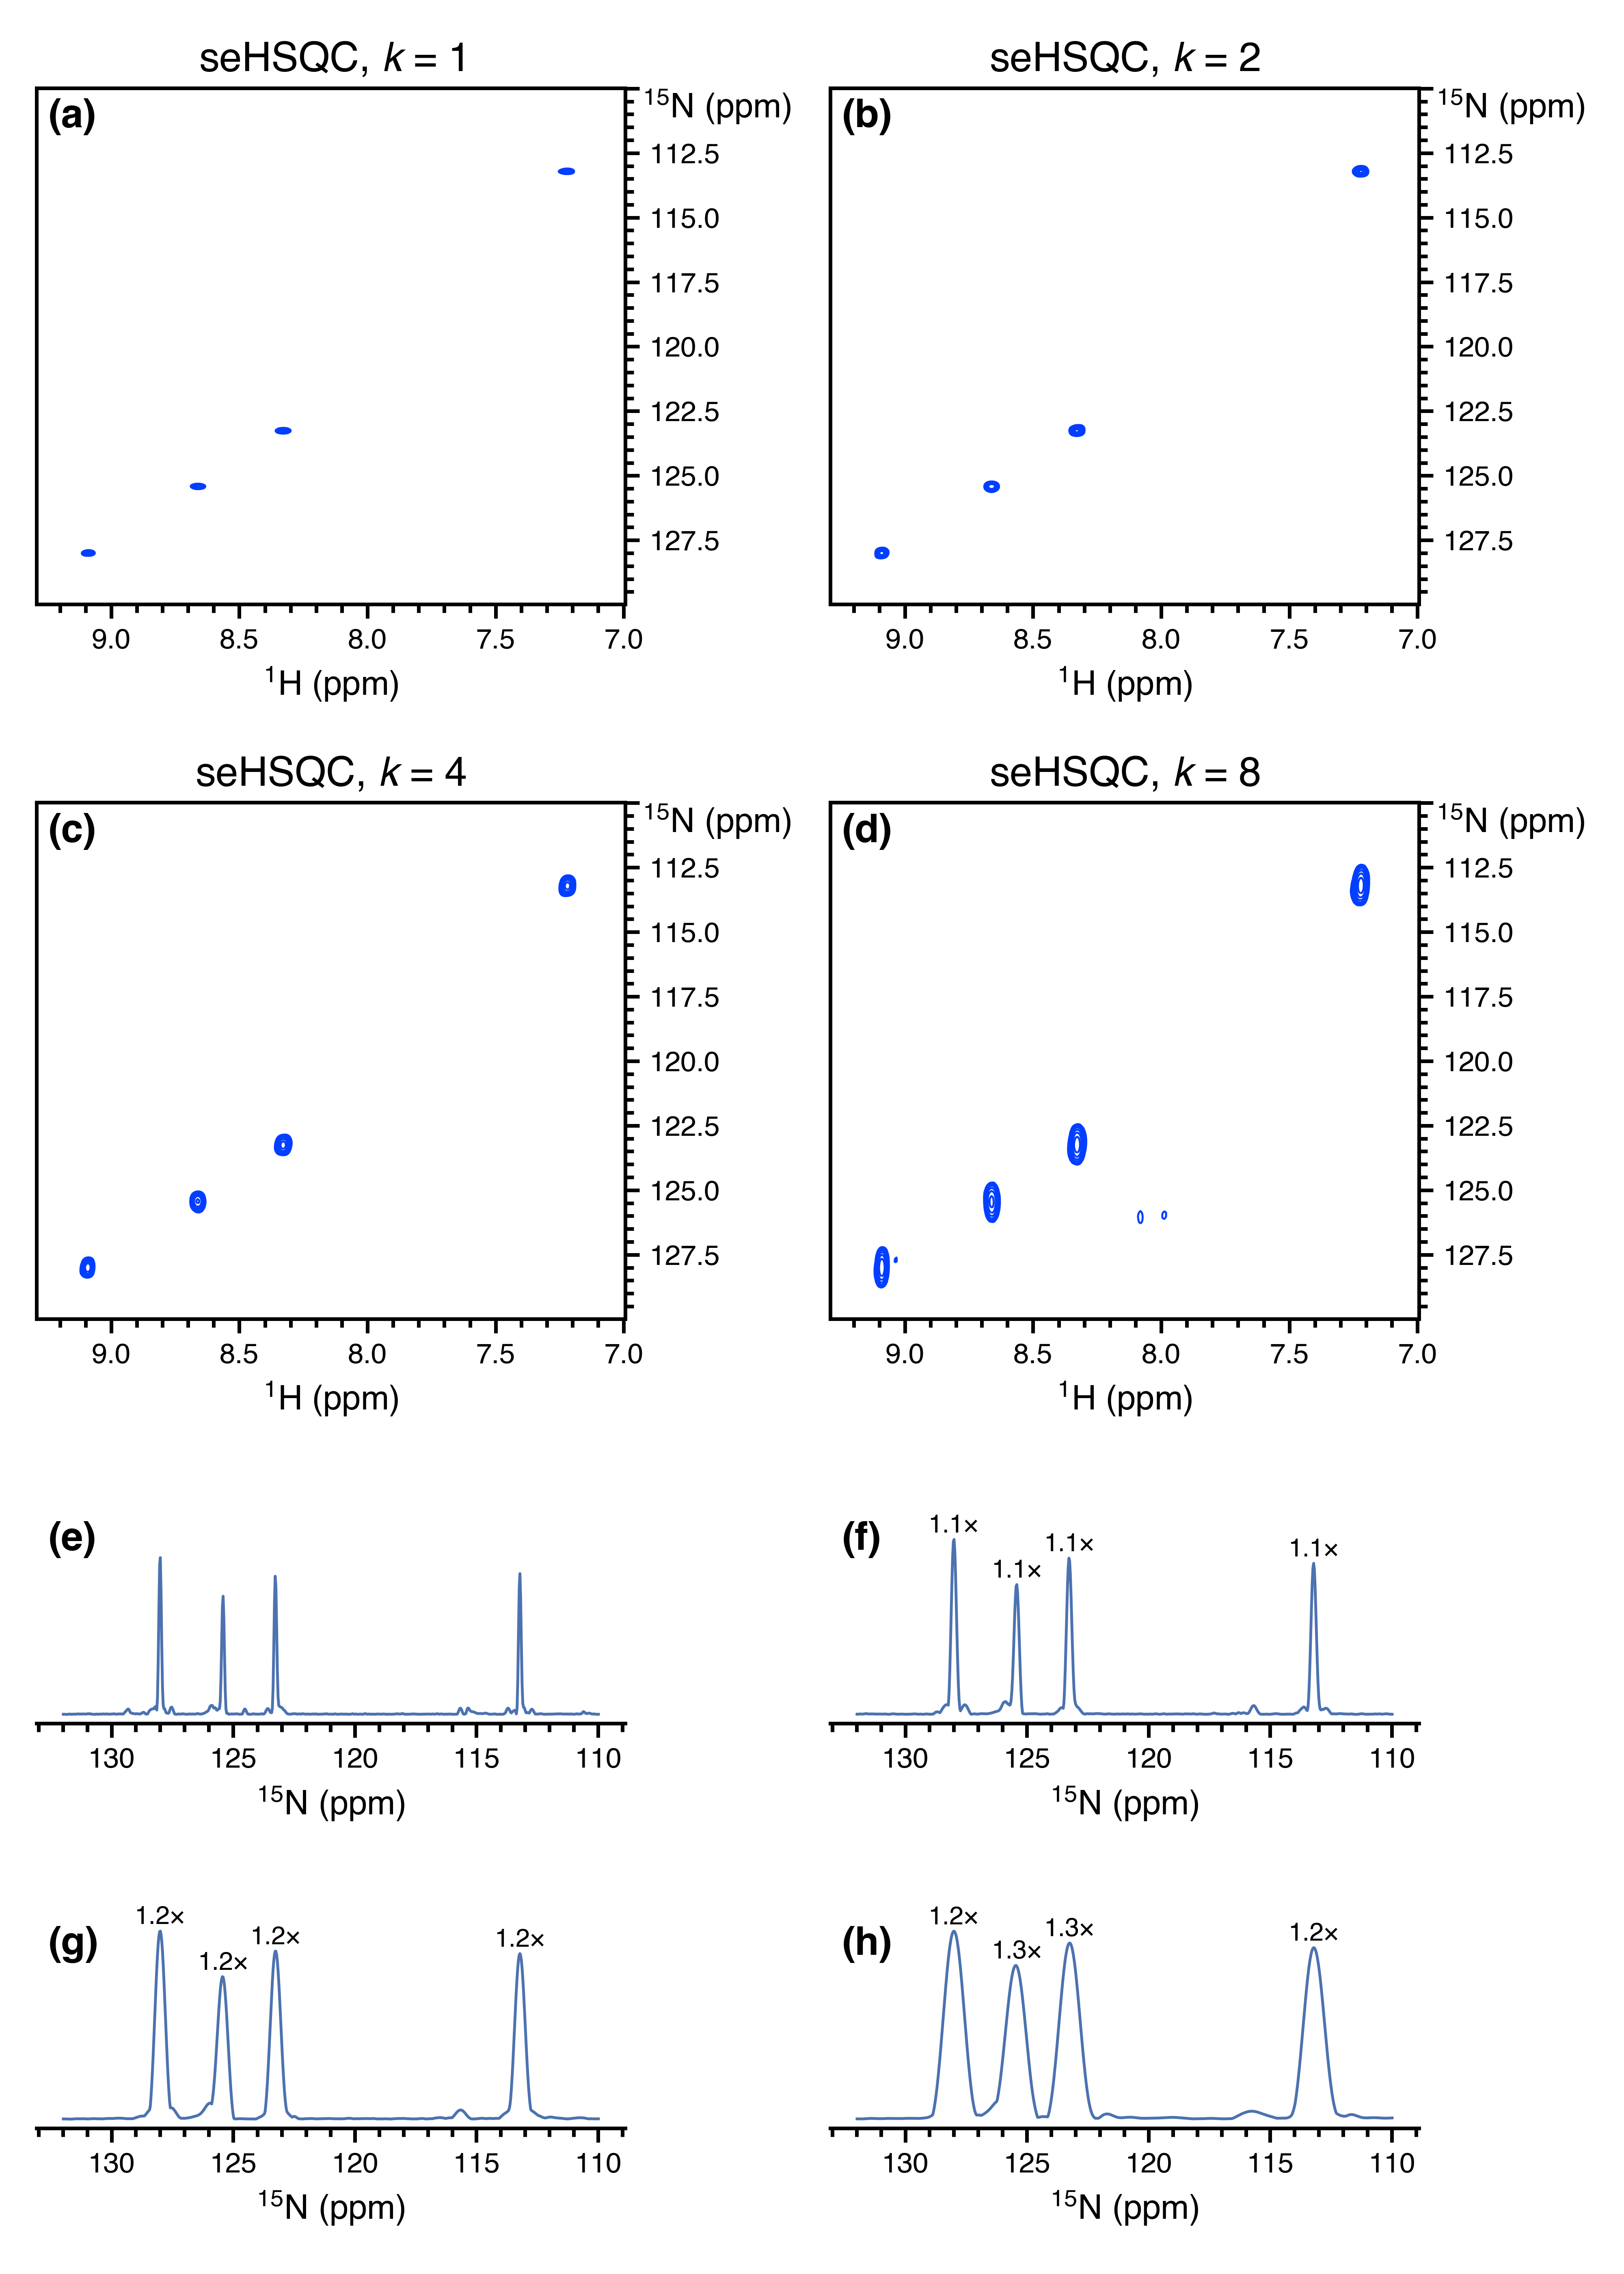
\includegraphics[width=\textwidth]{spv2_kscale.png}
    {\phantomsubcaption\label{fig:spv2_kscale_std}}
    {\phantomsubcaption\label{fig:spv2_kscale_k2}}
    {\phantomsubcaption\label{fig:spv2_kscale_k4}}
    {\phantomsubcaption\label{fig:spv2_kscale_k8}}
    {\phantomsubcaption\label{fig:spv2_kscale_sw2}}
    {\phantomsubcaption\label{fig:spv2_kscale_sw4}}
    {\phantomsubcaption\label{fig:spv2_kscale_sw8}}
    {\phantomsubcaption\label{fig:spv2_kscale_std_proj}}
    {\phantomsubcaption\label{fig:spv2_kscale_k2_proj}}
    {\phantomsubcaption\label{fig:spv2_kscale_k4_proj}}
    {\phantomsubcaption\label{fig:spv2_kscale_k8_proj}}
    {\phantomsubcaption\label{fig:spv2_kscale_sw2_proj}}
    {\phantomsubcaption\label{fig:spv2_kscale_sw4_proj}}
    {\phantomsubcaption\label{fig:spv2_kscale_sw8_proj}}
    \caption{
        \textbf{(seHSQC without extra linear prediction.)}
        \nitrogen{} seHSQC spectra taken from NOAH-3 \noahthree{Spn}{Spb}{Cc} supersequences.
        All spectra are plotted with the same noise levels.
        No linear prediction has been applied beyond the standard processing; thus, $\aqeff$ is $2 \times \mathrm{AQ}$ for all of the spectra above.
        \textbf{\subref{fig:spv2_kscale_std}} The ``standard'' spectrum.
        \textbf{\subref{fig:spv2_kscale_k2}} $k = 2$.
        \textbf{\subref{fig:spv2_kscale_k4}} $k = 4$.
        \textbf{\subref{fig:spv2_kscale_k8}} $k = 8$.
        \textbf{\subref{fig:spv2_kscale_sw2}} $\mathrm{SW} \times 2$.
        \textbf{\subref{fig:spv2_kscale_sw4}} $\mathrm{SW} \times 4$.
        \textbf{\subref{fig:spv2_kscale_sw8}} $\mathrm{SW} \times 8$.
        \textbf{\subref{fig:spv2_kscale_std_proj}}--\textbf{\subref{fig:spv2_kscale_sw8_proj}} Projections of 2D spectra in \subref{fig:spv2_kscale_std}--\subref{fig:spv2_kscale_sw8} onto the $f_1$ axis.
        Numbers indicate peak heights relative to the ``standard'' seHSQC spectrum in \subref{fig:spv2_kscale_std}.
        \grami{}
    }
    \label{fig:spv2_kscale}
\end{figure}

\begin{figure}
    \centering
    % figures/hmqc_kscale_lp.py
    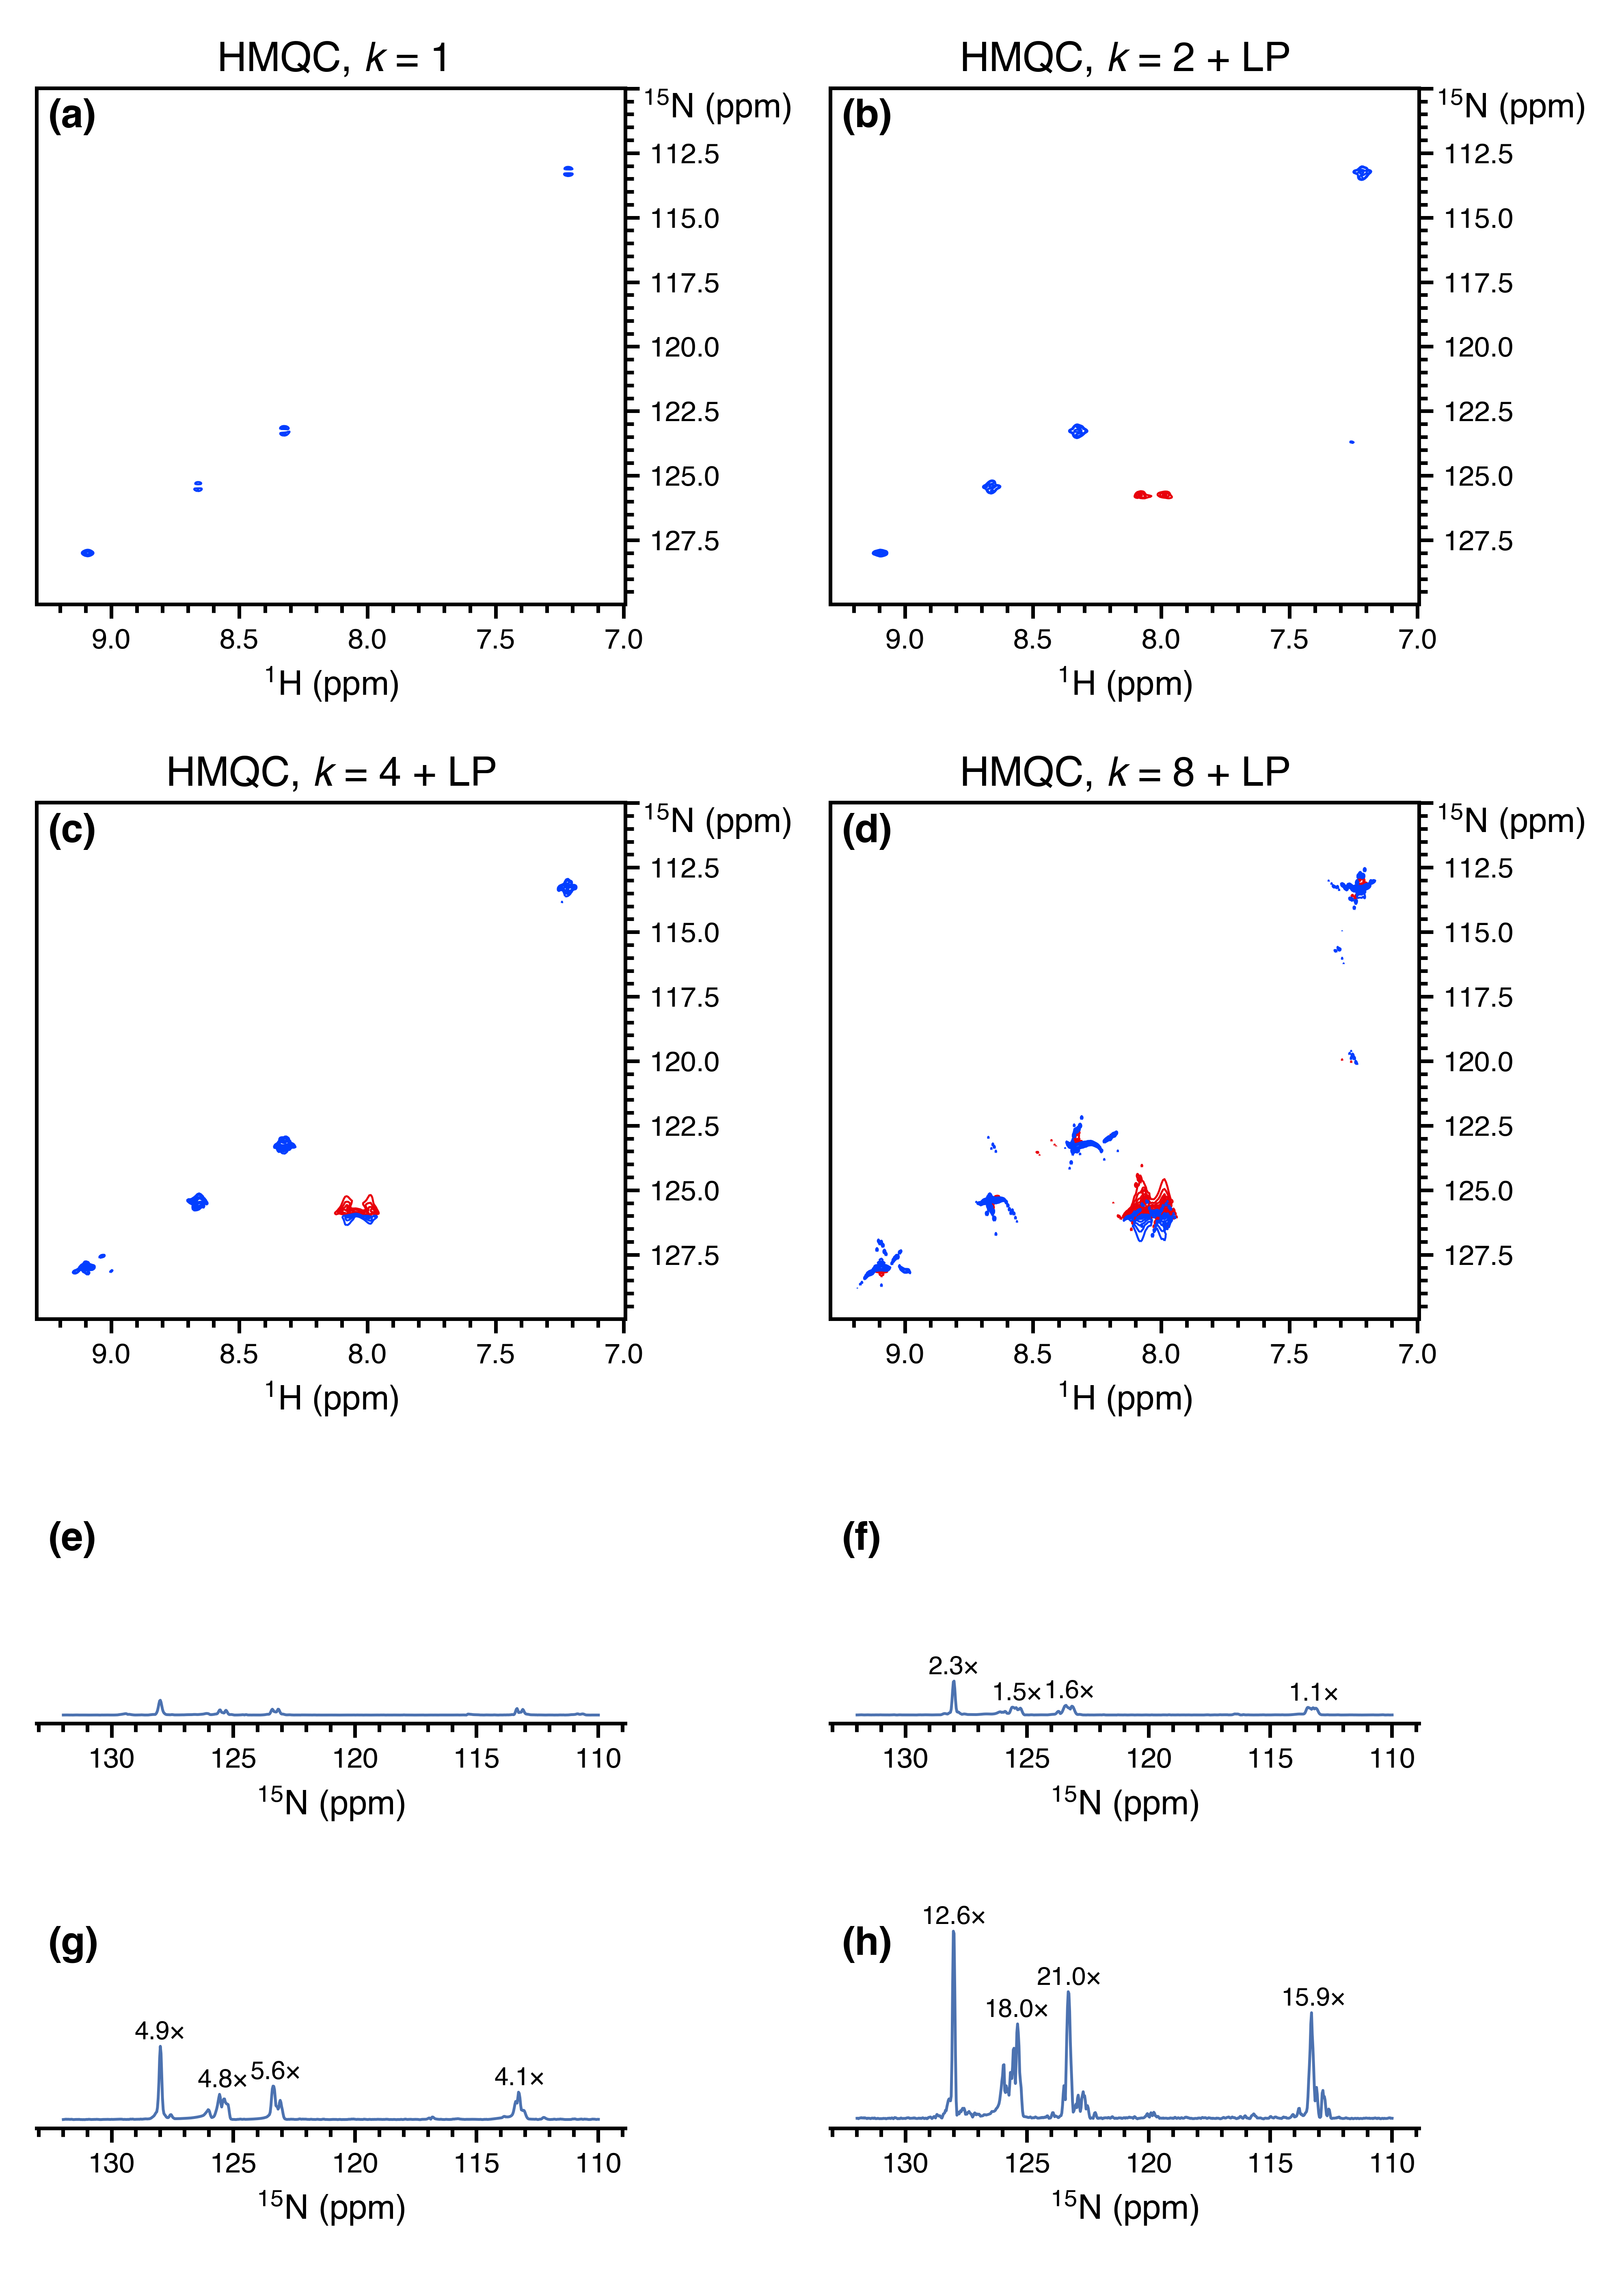
\includegraphics[width=\textwidth]{hmqc_kscale_lp.png}
    {\phantomsubcaption\label{fig:hmqc_kscale_lp_std}}
    {\phantomsubcaption\label{fig:hmqc_kscale_lp_k2}}
    {\phantomsubcaption\label{fig:hmqc_kscale_lp_k4}}
    {\phantomsubcaption\label{fig:hmqc_kscale_lp_k8}}
    {\phantomsubcaption\label{fig:hmqc_kscale_lp_sw2}}
    {\phantomsubcaption\label{fig:hmqc_kscale_lp_sw4}}
    {\phantomsubcaption\label{fig:hmqc_kscale_lp_sw8}}
    {\phantomsubcaption\label{fig:hmqc_kscale_lp_std_proj}}
    {\phantomsubcaption\label{fig:hmqc_kscale_lp_k2_proj}}
    {\phantomsubcaption\label{fig:hmqc_kscale_lp_k4_proj}}
    {\phantomsubcaption\label{fig:hmqc_kscale_lp_k8_proj}}
    {\phantomsubcaption\label{fig:hmqc_kscale_lp_sw2_proj}}
    {\phantomsubcaption\label{fig:hmqc_kscale_lp_sw4_proj}}
    {\phantomsubcaption\label{fig:hmqc_kscale_lp_sw8_proj}}
    \caption{
        \textbf{(HMQC with extra linear prediction.)}
        \nitrogen{} HMQC spectra taken from NOAH-3 \noahthree{M}{Spb}{Cc} supersequences.
        The datasets in this figure are the same as in \cref{fig:hmqc_kscale}: therefore, each column contains spectra which are \textit{acquired} with the same AQ.
        However, in this figure, all spectra have been subjected to time-domain linear prediction up to the same $\aqeff$ of \SI{120.3}{\ms}.
        \textbf{\subref{fig:hmqc_kscale_lp_std}} The ``standard'' spectrum.
        Note that this spectrum is identical to \cref{fig:hmqc_kscale_std}.
        \textbf{\subref{fig:hmqc_kscale_lp_k2}} $k = 2$.
        \textbf{\subref{fig:hmqc_kscale_lp_k4}} $k = 4$.
        \textbf{\subref{fig:hmqc_kscale_lp_k8}} $k = 8$.
        \textbf{\subref{fig:hmqc_kscale_lp_sw2}} $\mathrm{SW} \times 2$.
        \textbf{\subref{fig:hmqc_kscale_lp_sw4}} $\mathrm{SW} \times 4$.
        \textbf{\subref{fig:hmqc_kscale_lp_sw8}} $\mathrm{SW} \times 8$.
        \textbf{\subref{fig:hmqc_kscale_lp_std_proj}}--\textbf{\subref{fig:hmqc_kscale_lp_sw8_proj}} Projections of 2D spectra in \subref{fig:hmqc_kscale_lp_std}--\subref{fig:hmqc_kscale_lp_sw8} onto the $f_1$ axis.
        All spectra are plotted with the same noise levels.
        Note that linear prediction of $k$ times more points leads to a $\sqrt{k}$ increase in noise: so, for example, the projections in \subref{fig:hmqc_kscale_lp_k2_proj} and \subref{fig:hmqc_kscale_lp_sw2_proj} (with $k = 2$ and $\mathrm{SW \times 2}$ respectively) have $\sqrt{2}$ times more noise than the ``standard'' projection in \subref{fig:hmqc_kscale_lp_std_proj}.
        Numbers indicate signal-to-noise ratios relative to the ``standard'' HMQC spectrum in \subref{fig:hmqc_kscale_lp_std}, obtained by dividing the relative peak height by the increase in noise.
        The peak at $\delta_{\ce{H}} = \SI{8.03}{\ppm}$ is folded and therefore does not appear in the SW-scaled spectra.
        \grami{}
    }
    \label{fig:hmqc_kscale_lp}
\end{figure}

\begin{figure}
    \centering
    % figures/spv2_kscale_lp.py
    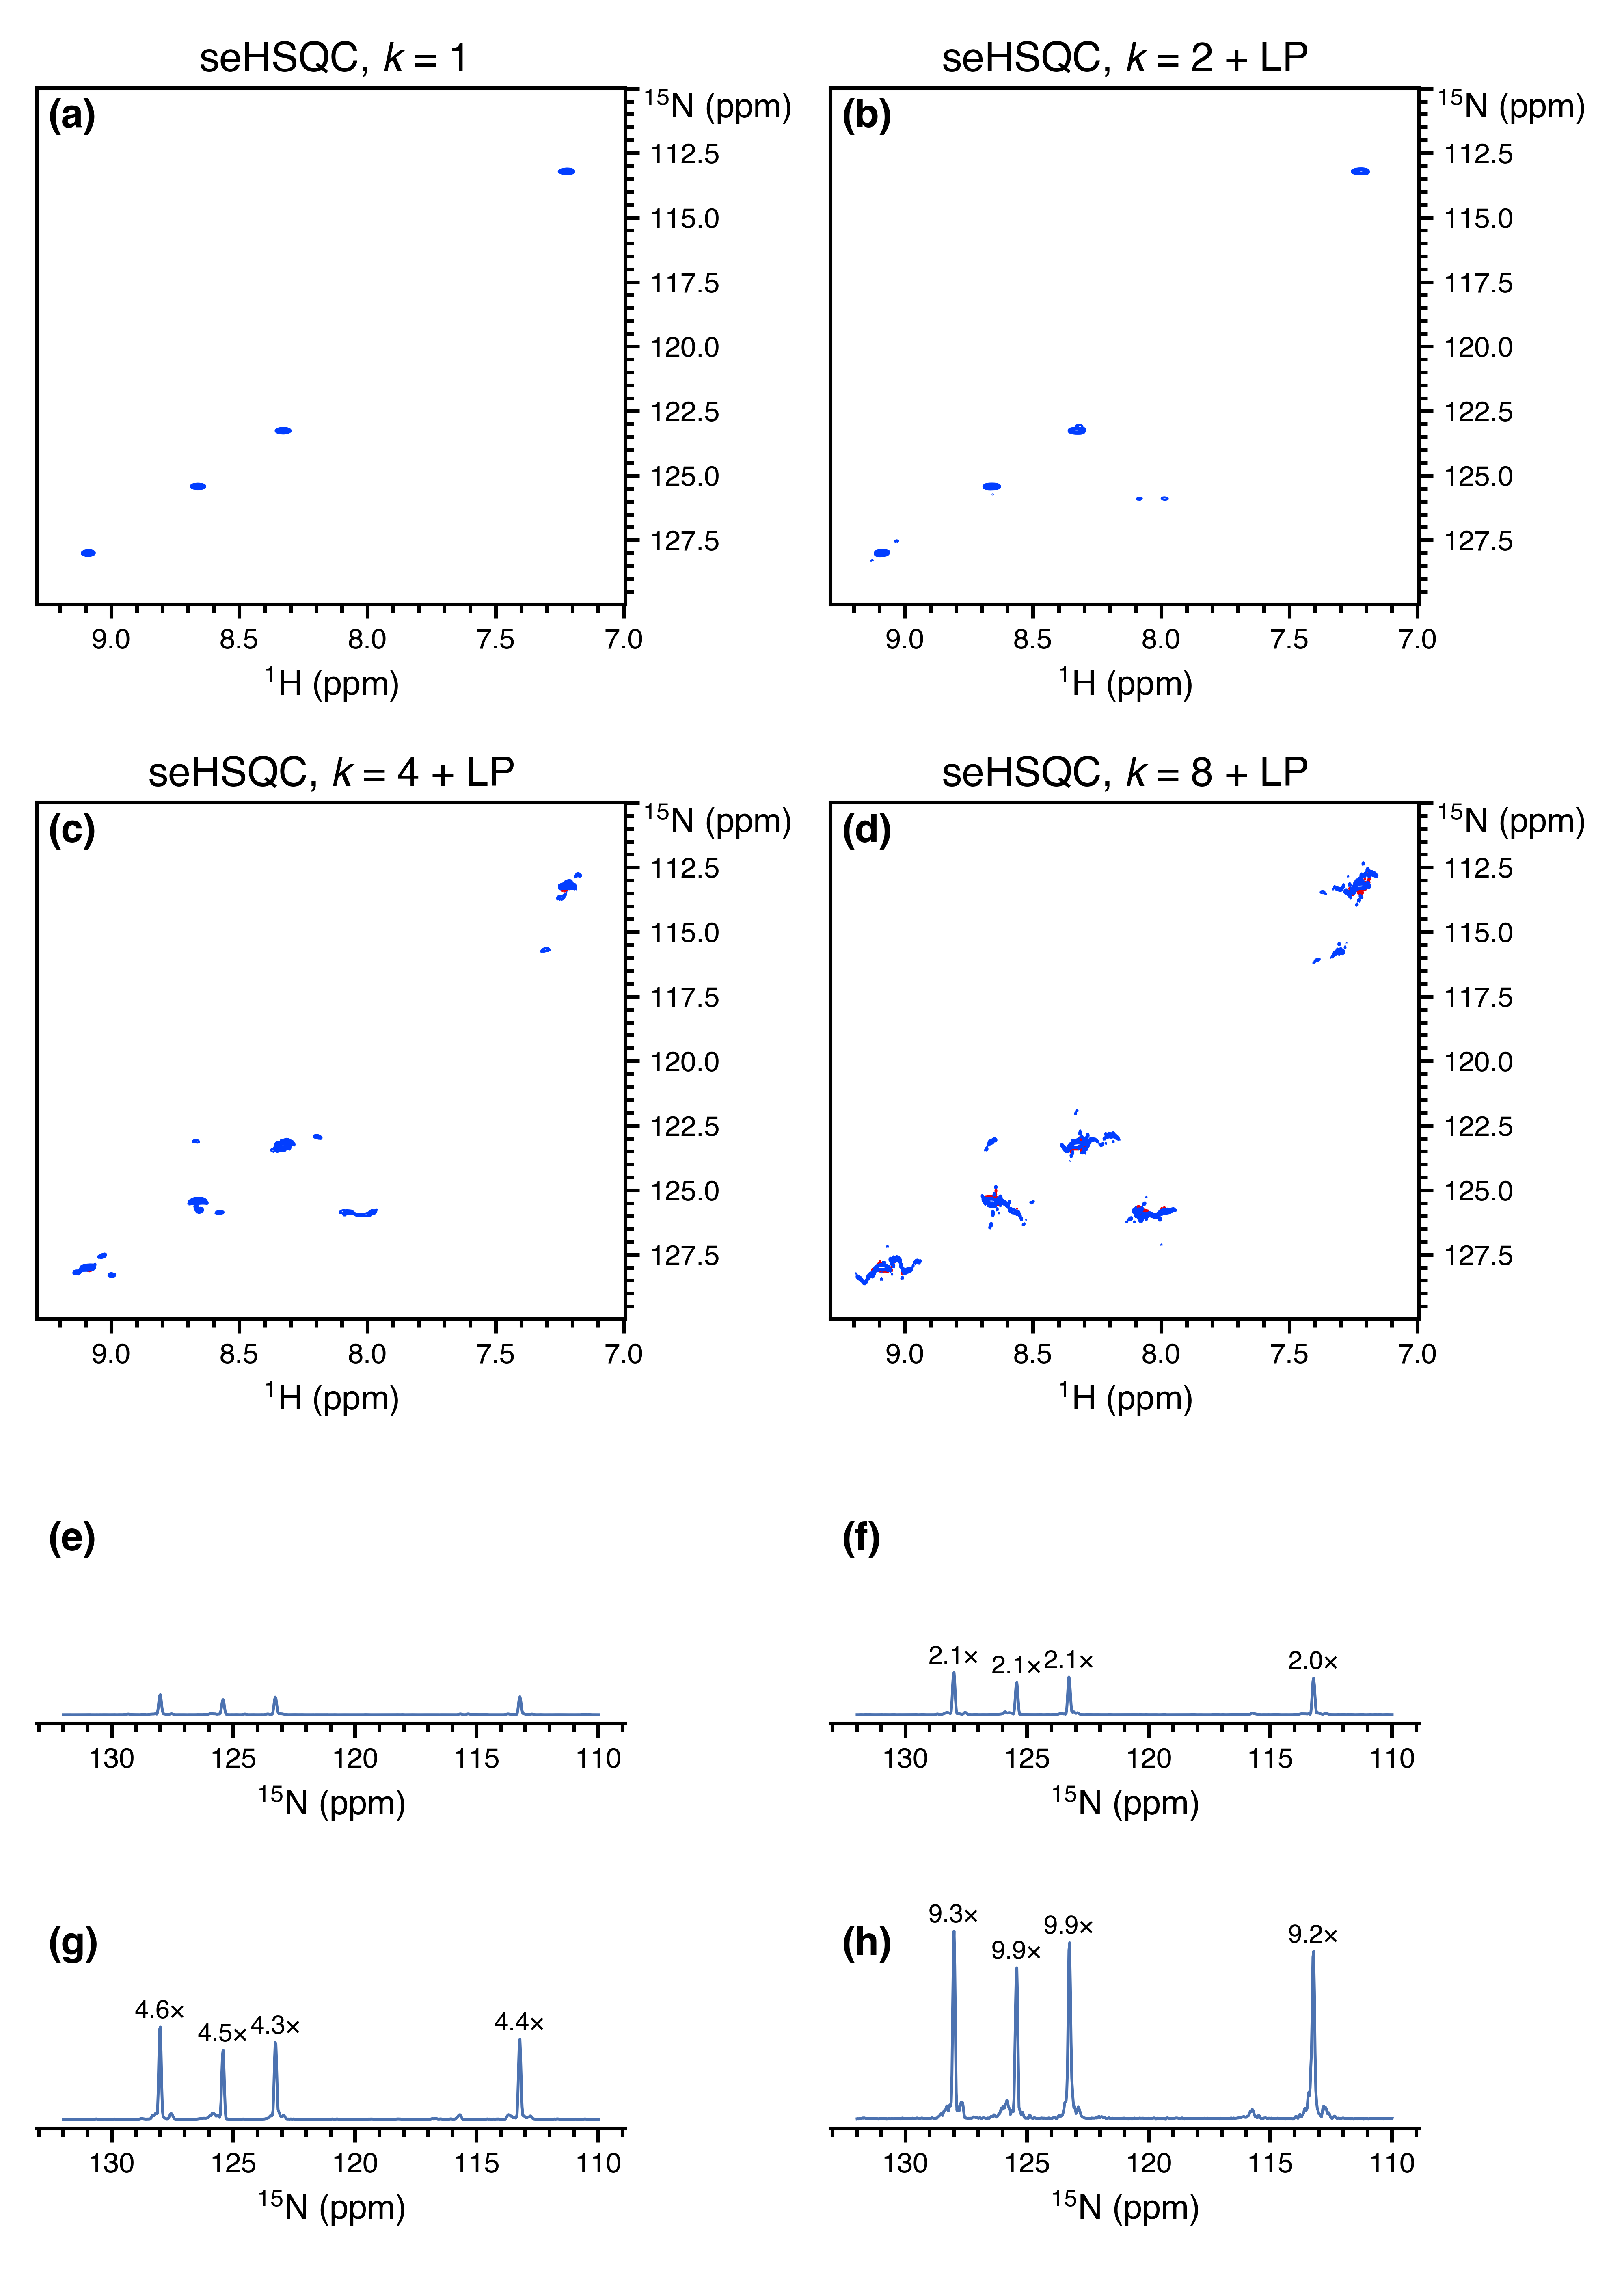
\includegraphics[width=\textwidth]{spv2_kscale_lp.png}
    {\phantomsubcaption\label{fig:spv2_kscale_lp_std}}
    {\phantomsubcaption\label{fig:spv2_kscale_lp_k2}}
    {\phantomsubcaption\label{fig:spv2_kscale_lp_k4}}
    {\phantomsubcaption\label{fig:spv2_kscale_lp_k8}}
    {\phantomsubcaption\label{fig:spv2_kscale_lp_sw2}}
    {\phantomsubcaption\label{fig:spv2_kscale_lp_sw4}}
    {\phantomsubcaption\label{fig:spv2_kscale_lp_sw8}}
    {\phantomsubcaption\label{fig:spv2_kscale_lp_std_proj}}
    {\phantomsubcaption\label{fig:spv2_kscale_lp_k2_proj}}
    {\phantomsubcaption\label{fig:spv2_kscale_lp_k4_proj}}
    {\phantomsubcaption\label{fig:spv2_kscale_lp_k8_proj}}
    {\phantomsubcaption\label{fig:spv2_kscale_lp_sw2_proj}}
    {\phantomsubcaption\label{fig:spv2_kscale_lp_sw4_proj}}
    {\phantomsubcaption\label{fig:spv2_kscale_lp_sw8_proj}}
    \caption{
        \textbf{(seHSQC with extra linear prediction.)}
        \nitrogen{} seHSQC spectra taken from NOAH-3 \noahthree{Spn}{Spb}{Cc} supersequences.
        The datasets in this figure are the same as in \cref{fig:spv2_kscale}: therefore, each column contains spectra which are \textit{acquired} with the same AQ.
        However, in this figure, \textbf{all spectra have been subjected to time-domain linear prediction} up to the same $\aqeff$ of \SI{120.3}{\ms}.
        \textbf{\subref{fig:spv2_kscale_lp_std}} The ``standard'' spectrum with $\mathrm{SW} = \SI{30}{\ppm}$, $k = 1$, 256 $t_1$ increments (linear predicted to 512 indirect-dimension points), and 2 scans per increment (denoted as $30:256:2$; AQ = \SI{60.1}{\ms}).
        \textbf{\subref{fig:spv2_kscale_lp_std}} The ``standard'' spectrum.
        Note that this spectrum is identical to \cref{fig:spv2_kscale_std}.
        \textbf{\subref{fig:spv2_kscale_lp_k2}} $k = 2$.
        \textbf{\subref{fig:spv2_kscale_lp_k4}} $k = 4$.
        \textbf{\subref{fig:spv2_kscale_lp_k8}} $k = 8$.
        \textbf{\subref{fig:spv2_kscale_lp_sw2}} $\mathrm{SW} \times 2$.
        \textbf{\subref{fig:spv2_kscale_lp_sw4}} $\mathrm{SW} \times 4$.
        \textbf{\subref{fig:spv2_kscale_lp_sw8}} $\mathrm{SW} \times 8$.
        \textbf{\subref{fig:spv2_kscale_lp_std_proj}}--\textbf{\subref{fig:spv2_kscale_lp_sw8_proj}} Projections of 2D spectra in \subref{fig:spv2_kscale_lp_std}--\subref{fig:spv2_kscale_lp_sw8} onto the $f_1$ axis.
        All spectra are plotted with the same noise levels.
        Note that linear prediction of $k$ times more points leads to a $\sqrt{k}$ increase in noise: so, for example, the projections in \subref{fig:spv2_kscale_lp_k2_proj} and \subref{fig:spv2_kscale_lp_sw2_proj} (with $k = 2$ and $\mathrm{SW \times 2}$ respectively) have $\sqrt{2}$ times more noise than the ``standard'' projection in \subref{fig:spv2_kscale_lp_std_proj}.
        Numbers indicate signal-to-noise ratios relative to the ``standard'' seHSQC spectrum in \subref{fig:spv2_kscale_lp_std}, obtained by dividing the relative peak height by the increase in noise.
        The peak at $\delta_{\ce{H}} = \SI{8.03}{\ppm}$ is folded and therefore does not appear in the SW-scaled spectra.
        \grami{}
    }
    \label{fig:spv2_kscale_lp}
\end{figure}

\section{HSQC-TOCSY/HSQC sensitivity comparisons}

The signal intensities for the NOAH-3 \noahthree{St}{S}{Cc} (HSQC-TOCSY + HSQC + CLIP-COSY) supersequences can be more conveniently measured by omitting the DIPSI-2 isotropic mixing in the HSQC-TOCSY supersequence, leading to a NOAH-3 \noahthree{S}{S}{Cc} (HSQC + HSQC + CLIP-COSY) supersequence.
This allows us to compare the different versions of double-HSQC sequences, as the two HSQC modules can be implemented either using the MFA approach, or the new ASAP/NOAH approach based on Ernst angle excitation in the first module.
In the latter implementation, the parameter $f$ can be varied between 0.4 and 1; it represents the proportion of \magn{\ce{C}} magnetisation used in the first HSQC, as described in the main text.
Furthermore, to boost the sensitivity of the second HSQC module in the NOAH supersequences, either of the two new seHSQC modules can be used in its place: we demonstrate this here with the ZIP-seHSQC (\noahSpb{}).

\begin{figure}
    \centering
    % figures/ssc_comparisons.py
    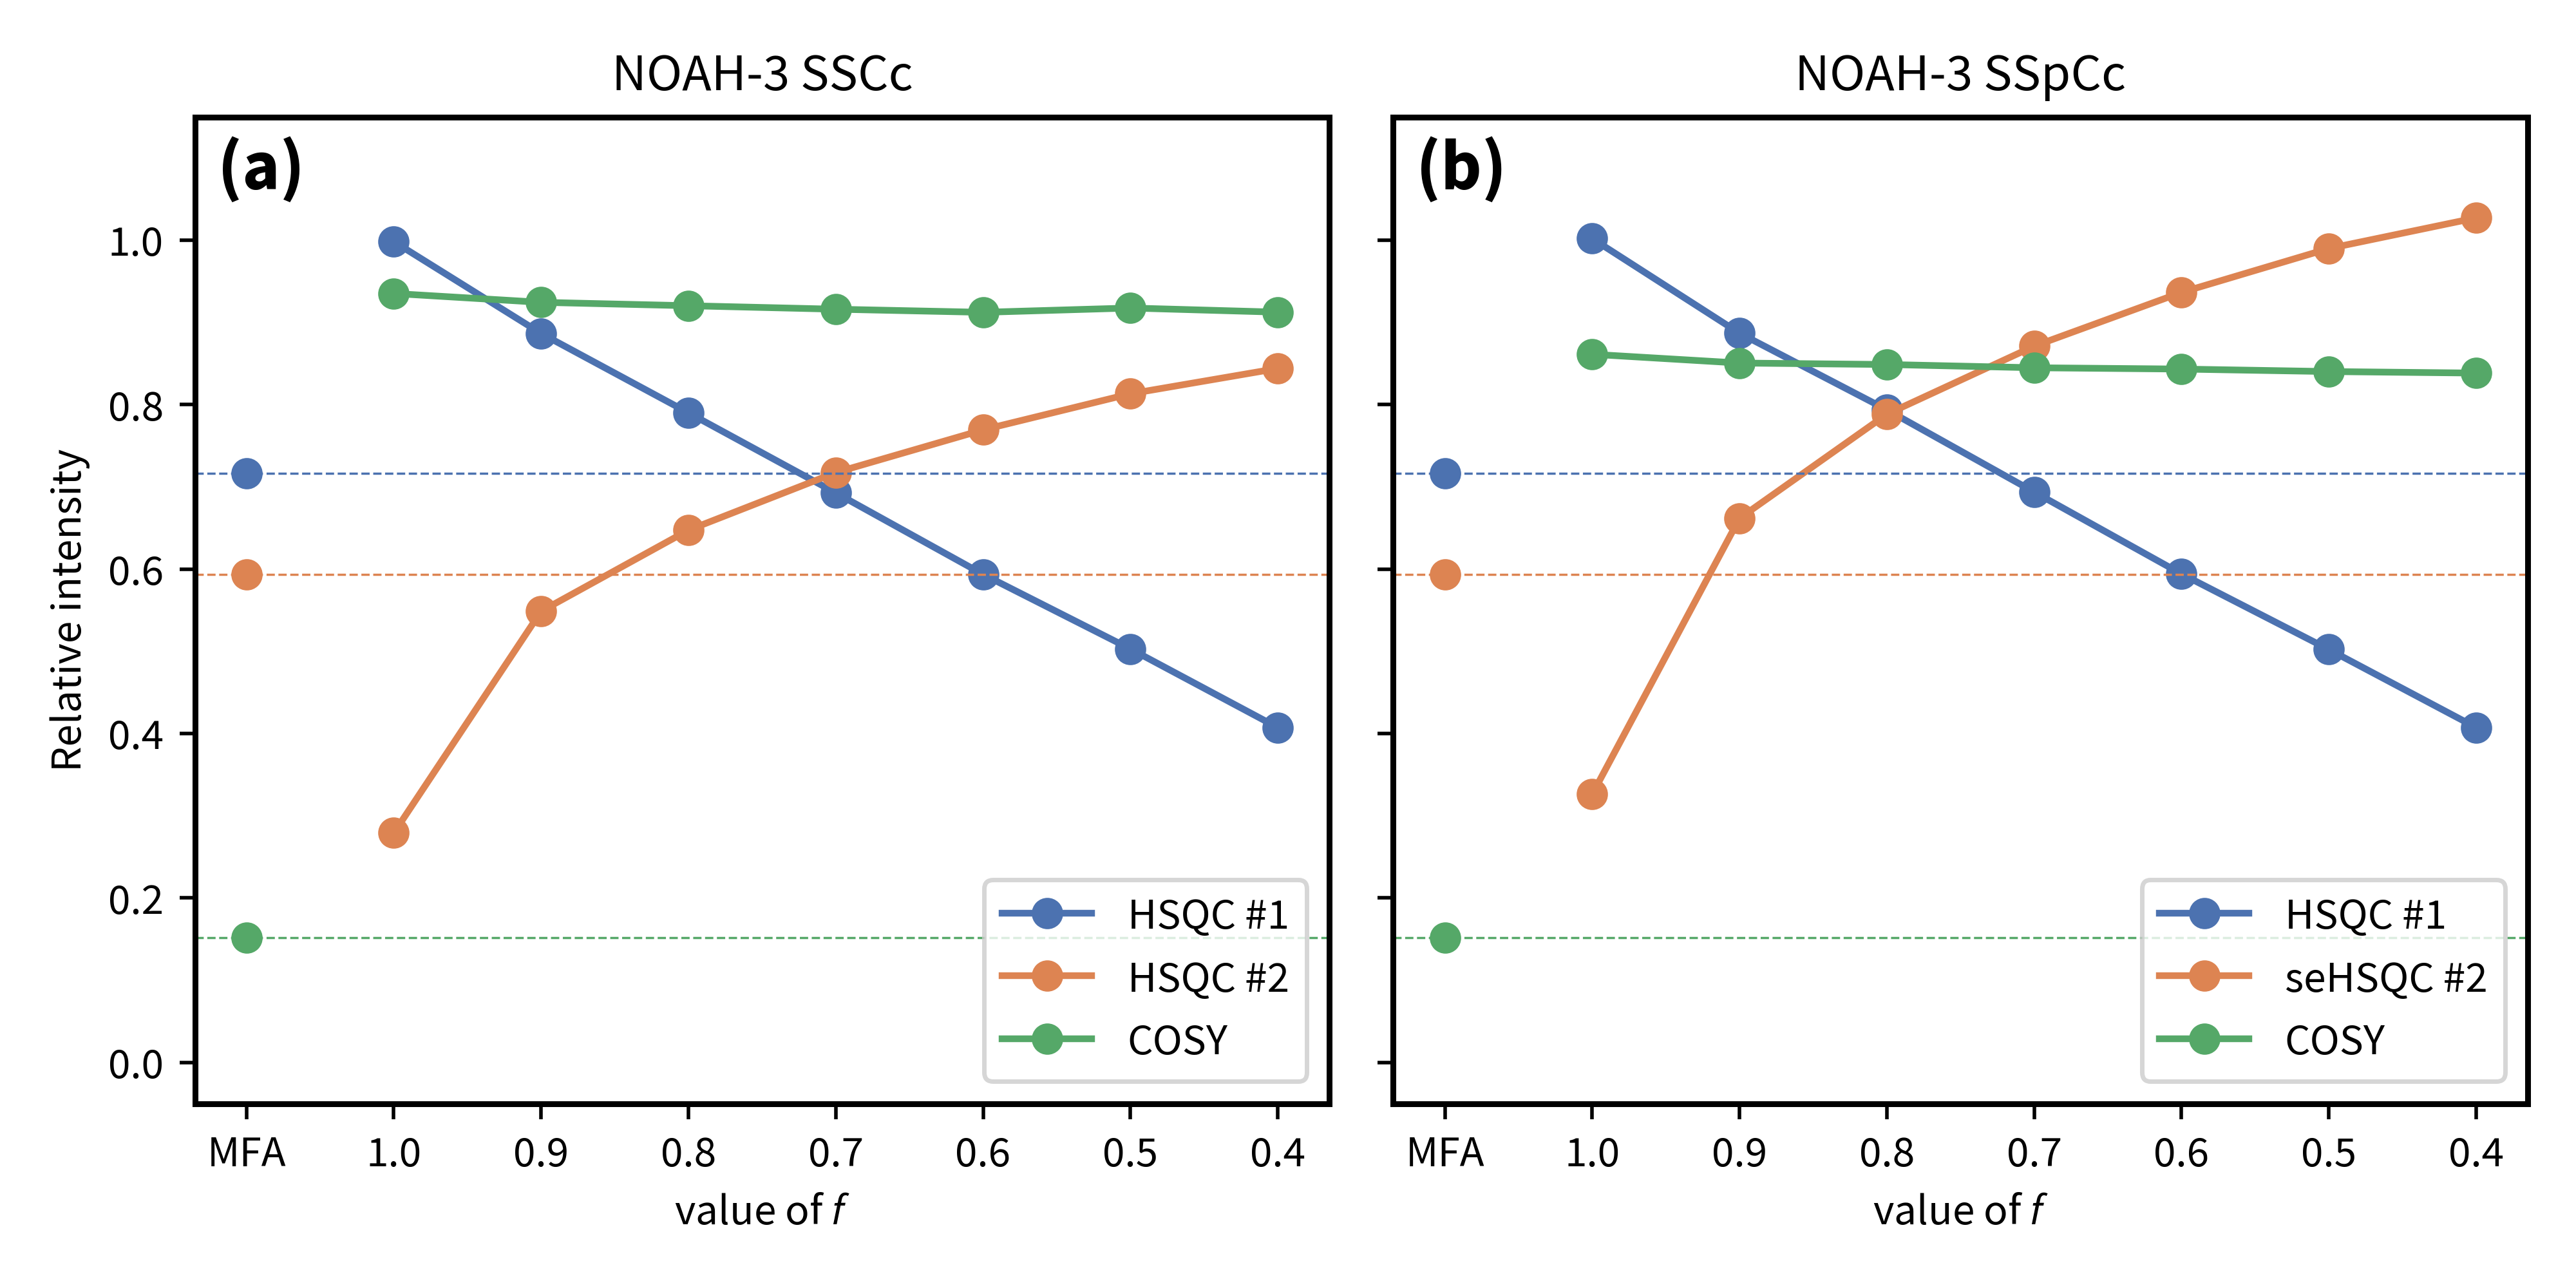
\includegraphics[width=0.8\textwidth]{ssc_comparisons.png}
    \caption{
        Sensitivities of HSQC and CLIP-COSY modules when used as part of a \noahthree{S}{S}{Cc}-type supersequence, with both the NOAH and MFA implementations of the two HSQC modules.
        Intensities are calculated relative to the HSQC and CLIP-COSY modules in a standard NOAH-2 SCc supersequence (averaged over all peaks).
        \textbf{(a)} Sensitivity of the MFA implementation (i.e.\ a MFA double HSQC experiment immediately followed by a CLIP-COSY).
        Horizontal dashed lines at these levels are drawn across all subplots to guide the eye.
        \textbf{(b)} Sensitivity of NOAH-3 \noahthree{S}{S}{Cc} modules as a function of $f$.
        Note that at $f = 0.8$, all of the NOAH spectra have a greater average sensitivity than their MFA counterparts.
        \textbf{(c)} Sensitivity of NOAH-3 \noahthree{S}{Spb}{Cc} modules as a function of $f$.
        \andro{}
    }
    \label{fig:ssc_comparisons}
\end{figure}

\cref{fig:ssc_comparisons} may be understood in the following way:

\begin{itemize}
    \item The MFA HSQC sensitivities (in (a)) are approximately half that of a standard CRK seHSQC, with the second HSQC having slightly lower sensitivity.\autocite{Nolis2019CPC}
    \item The sensitivity of the first NOAH HSQC (blue in (b) and (c)) is generally equal to $f$, supporting the interpretation of $f$ as the fraction of \magn{\ce{C}} magnetisation excited in the first HSQC.
    \item The sensitivity of the second NOAH HSQC (orange in (b)) arises from whatever is \textit{not} used by the first HSQC, plus any magnetisation that recovers during the FID of the first HSQC.
        As $f$ is decreased, the former contribution increases and the latter tapers off.
        This is true for the seHSQC as well (orange in (c)), except that there is a uniform boost in sensitivity for all values of $f$.
        This sensitivity improvement mainly applies to \ce{CH} groups, as discussed in the main text.
    \item The MFA COSY sensitivity (green) is substantially lower ($\sim 15\%$) because the bulk magnetisation is dephased by the previous modules, whereas in the NOAH approach it is (largely) preserved.
\end{itemize}

It remains to evaluate the impact of adding DIPSI-2 mixing in one of the HSQC modules on the remaining modules in the supersequence.
This depends on whether the HSQC-TOCSY module is placed first (\noahthree{St}{S}{Cc} or \noahthree{St}{Sp}{Cc}) or second (\noahthree{S}{St}{Cc}) in the sequence.
Since neither of the new seHSQC modules do preserve unused \magn{\ce{C}} magnetisation, the HSQC-TOCSY in a hypothetical \noahthree{Sp}{St}{Cc} supersequence will have greatly reduced sensitivity.
On the other hand, placing the HSQC-TOCSY sequence first allows the seHSQC module to be used subsequent to this; we therefore consider only the permutations where the HSQC-TOCSY goes first.

\begin{figure}
    \centering
    % figures/stsc_comparisons.py
    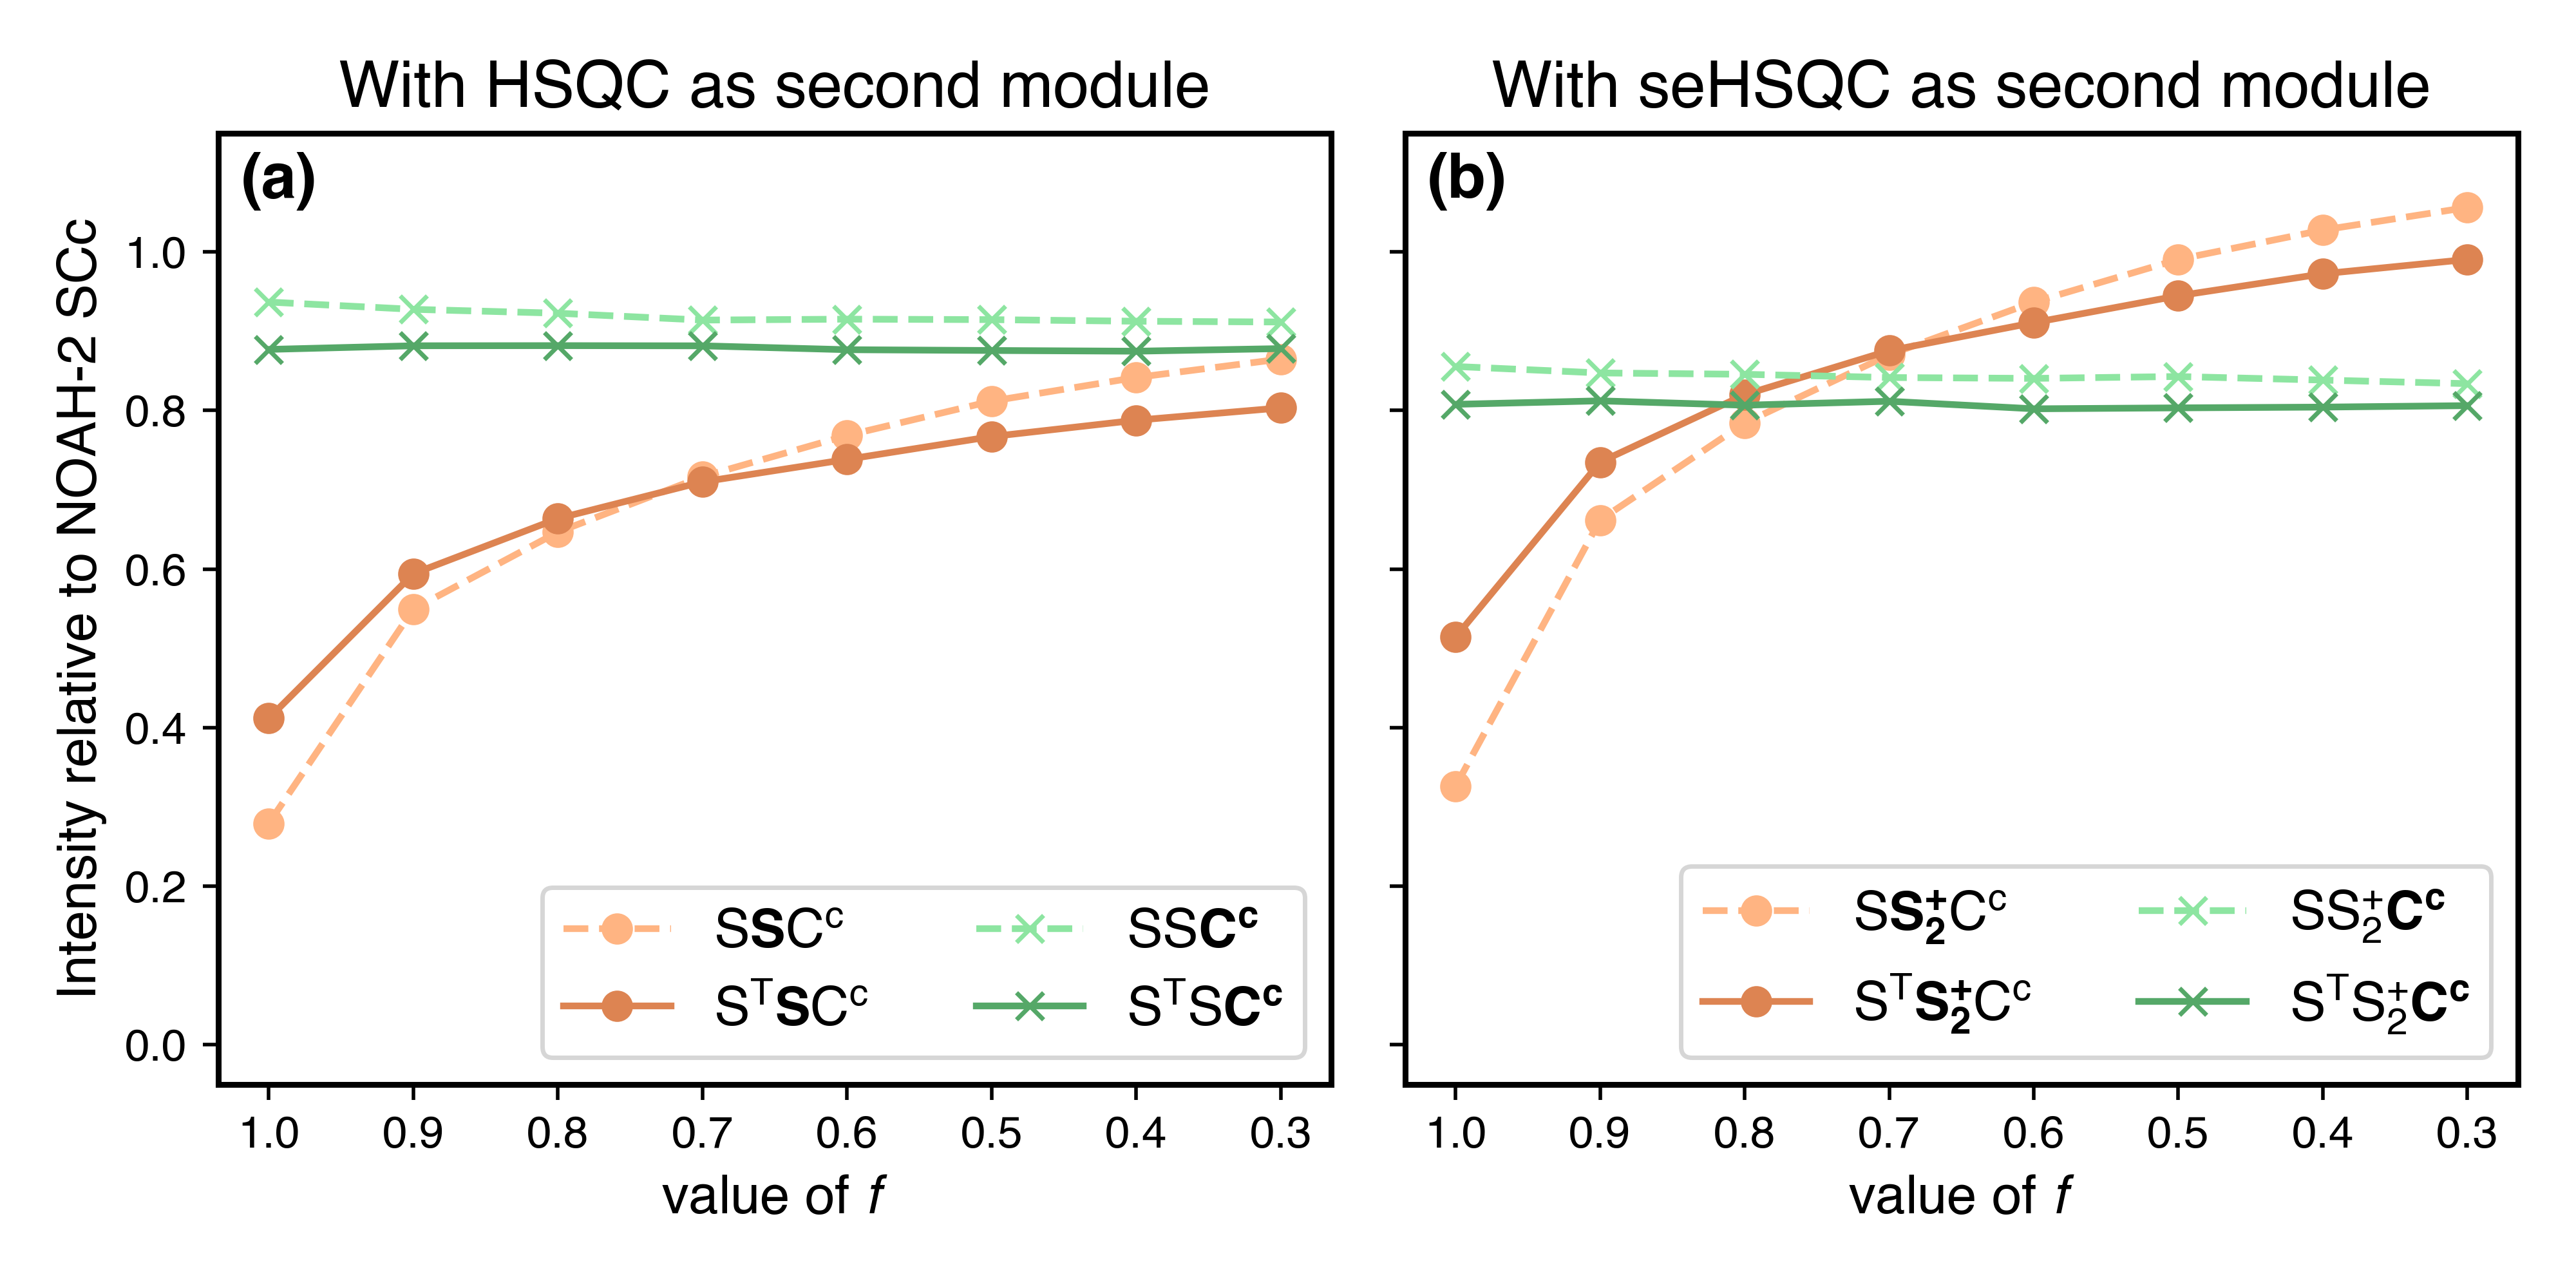
\includegraphics[width=0.8\textwidth]{stsc_comparisons.png}
    \caption{
        Comparison of signal intensities of second (HSQC or seHSQC) and third (CLIP-COSY) modules in the \noahthree{St}{S}{Cc} and \noahthree{St}{Spb}{Cc} supersequences, versus their intensities in the \noahthree{S}{S}{Cc} and \noahthree{S}{Spb}{Cc} sequences, as a function of the parameter $f$.
        The solid, darker lines indicate the supersequences beginning with the HSQC-TOCSY, whereas the dashed, lighter lines indicate the supersequences beginning with the HSQC (the latter are the same graphs as in \cref{fig:ssc_comparisons}).
        \textbf{(a)} With the HSQC as the second module.
        \textbf{(b)} With the seHSQC as the second module.
        \andro{}
    }
    \label{fig:stsc_comparisons}
\end{figure}

It can be seen from \cref{fig:stsc_comparisons} that the introduction of DIPSI-2 mixing leads to a very small drop ($< 10\%$) in the amount of \magnnot{\ce{C}} magnetisation preserved for the COSY module.
On the other hand, the HSQC (and seHSQC) sensitivites follow largely the same trend as before.
For values of $f$ above $0.7$ (where relatively little \magn{\ce{C}} magnetisation is preserved for these modules), the DIPSI-2 mixing helps to replenish some of this magnetisation.
As $f$ decreases, this effect becomes smaller, and at $f < 0.7$ it even leads to a \textit{reduction} in signal intensity (i.e.\ where the orange lines cross in \cref{fig:stsc_comparisons}).

As discussed in the main text, since the HSQC-TOCSY has a lower intrinsic sensitivity than the (se)HSQC, we recommend using a large value of $f$, such as $0.9$.
This does not compromise the HSQC-TOCSY intensity by much, and at the same time yields either a HSQC with $\sim 60\%$ of its original sensitivity, or a seHSQC which has $\sim 75\%$ of the sensitivity of a standalone NOAH HSQC module.
However, if the sensitivity of the HSQC-TOCSY component is to be maximised, then it is advisable to use the seHSQC-TOCSY module, which is based on the \noahSpb{} module.\autocite{Hansen2021AC}
This module cannot preserve any \magn{\ce{C}} magnetisation for the downstream HSQC, but does retain \magnnot{\ce{C}} magnetisation for homonuclear modules: its performance in this respect is therefore very similar to the HSQC-TOCSY with $f = 1$ (\cref{fig:sehsqc_tocsy}).
However, it provides greater sensitivity in the HSQC-TOCSY component itself, so is strictly better than the HSQC-TOCSY with $f = 1$.

\begin{figure}
    \centering
    % figures/sehsqc_tocsy.py
    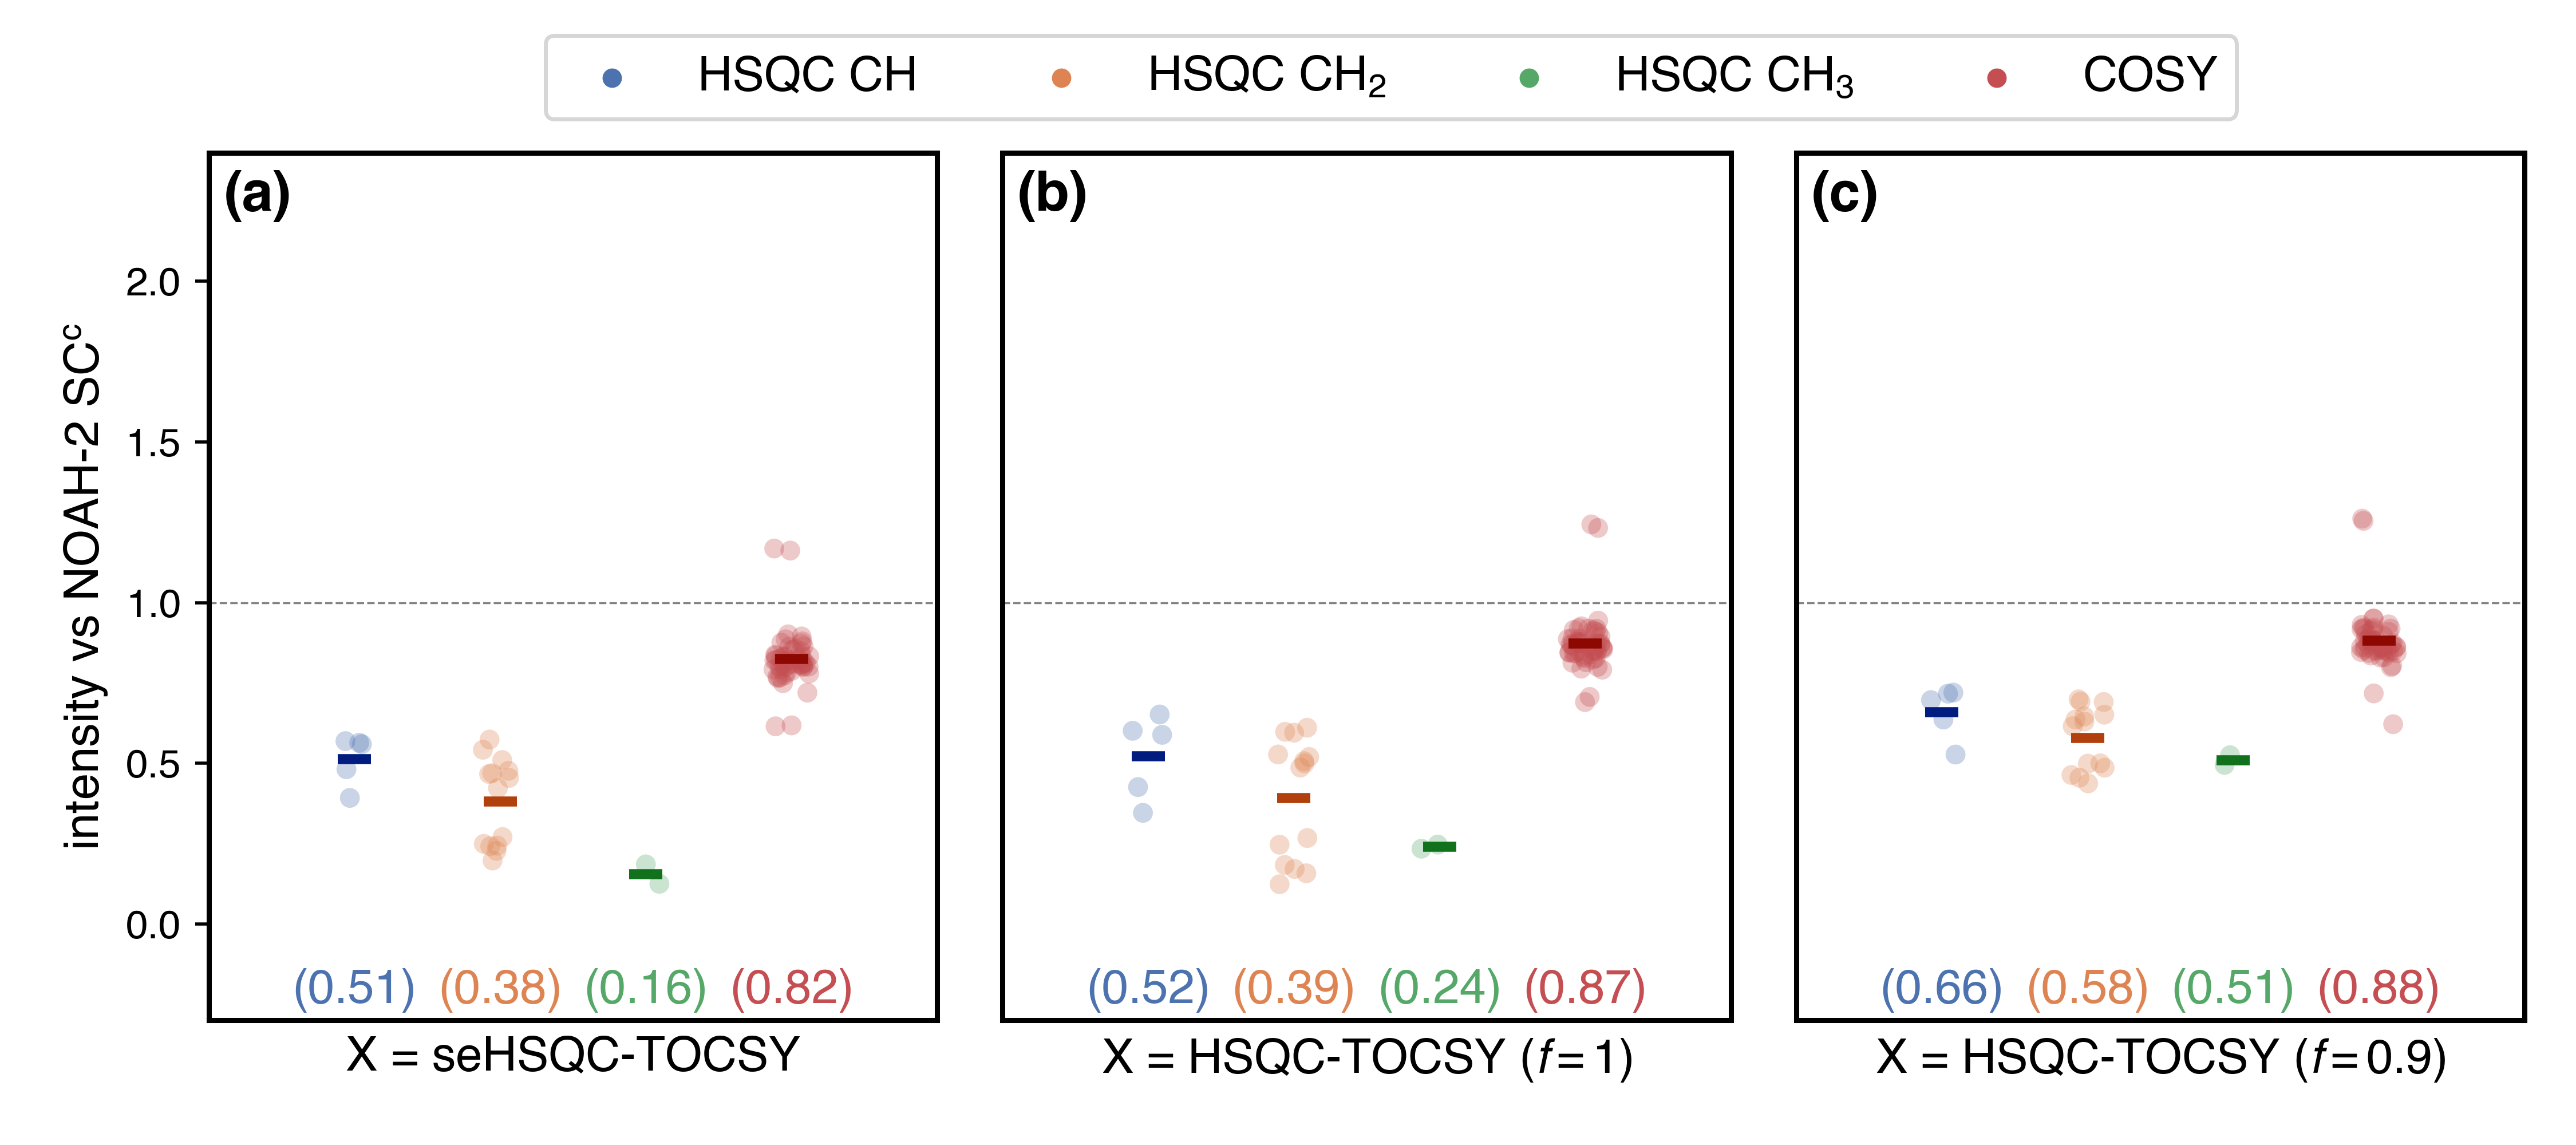
\includegraphics[width=0.8\textwidth]{sehsqc_tocsy.png}
    \caption{
        HSQC and COSY intensities in NOAH-3 \noahthree{X}{S}{Cc} supersequences, where \noahX{} is a HSQC-TOCSY variant, normalised against the intensities of the NOAH-2 \noahtwo{S}{Cc}.
        \textbf{(a)} With X as the seHSQC-TOCSY module, derived from the \noahSpb{} sequence.
        \textbf{(b)} With the unenhanced HSQC-TOCSY module ($f = 1$). Note that this provides no improvement over the seHSQC-TOCSY in the downstream HSQC and COSY modules.
        \textbf{(c)} With the unenhanced HSQC-TOCSY module ($f = 0.9$). This retains a portion of unused \magn{\ce{C}} magnetisation for the second HSQC, resulting in higher intensities.
        \andro{}
    }
    \label{fig:sehsqc_tocsy}
\end{figure}

Finally, we note that because a significant proportion of the HSQC signal derives from \magn{\ce{C}} relaxation during the HSQC-TOCSY FID, use of a longer AQ can potentially boost the HSQC sensitivity even further.
The experiments shown above were carried out with a relatively short AQ of \SI{73}{\ms}.
\textbf{However, bear in mind that the high duty cycle associated with broadband \ce{^13C} decoupling can potentially damage the probe if applied for too long, especially given that the supersequences described here have two consecutive \ce{^13C}-decoupled modules, as well as a \ce{^1H} isotropic mixing period.}

\section{Other example spectra}
\label{section:si_spectra}

\begin{figure}
    \centering
    % figures/stspct.py
    
\includegraphics{andro.png}\phantom{aaaaaa}
    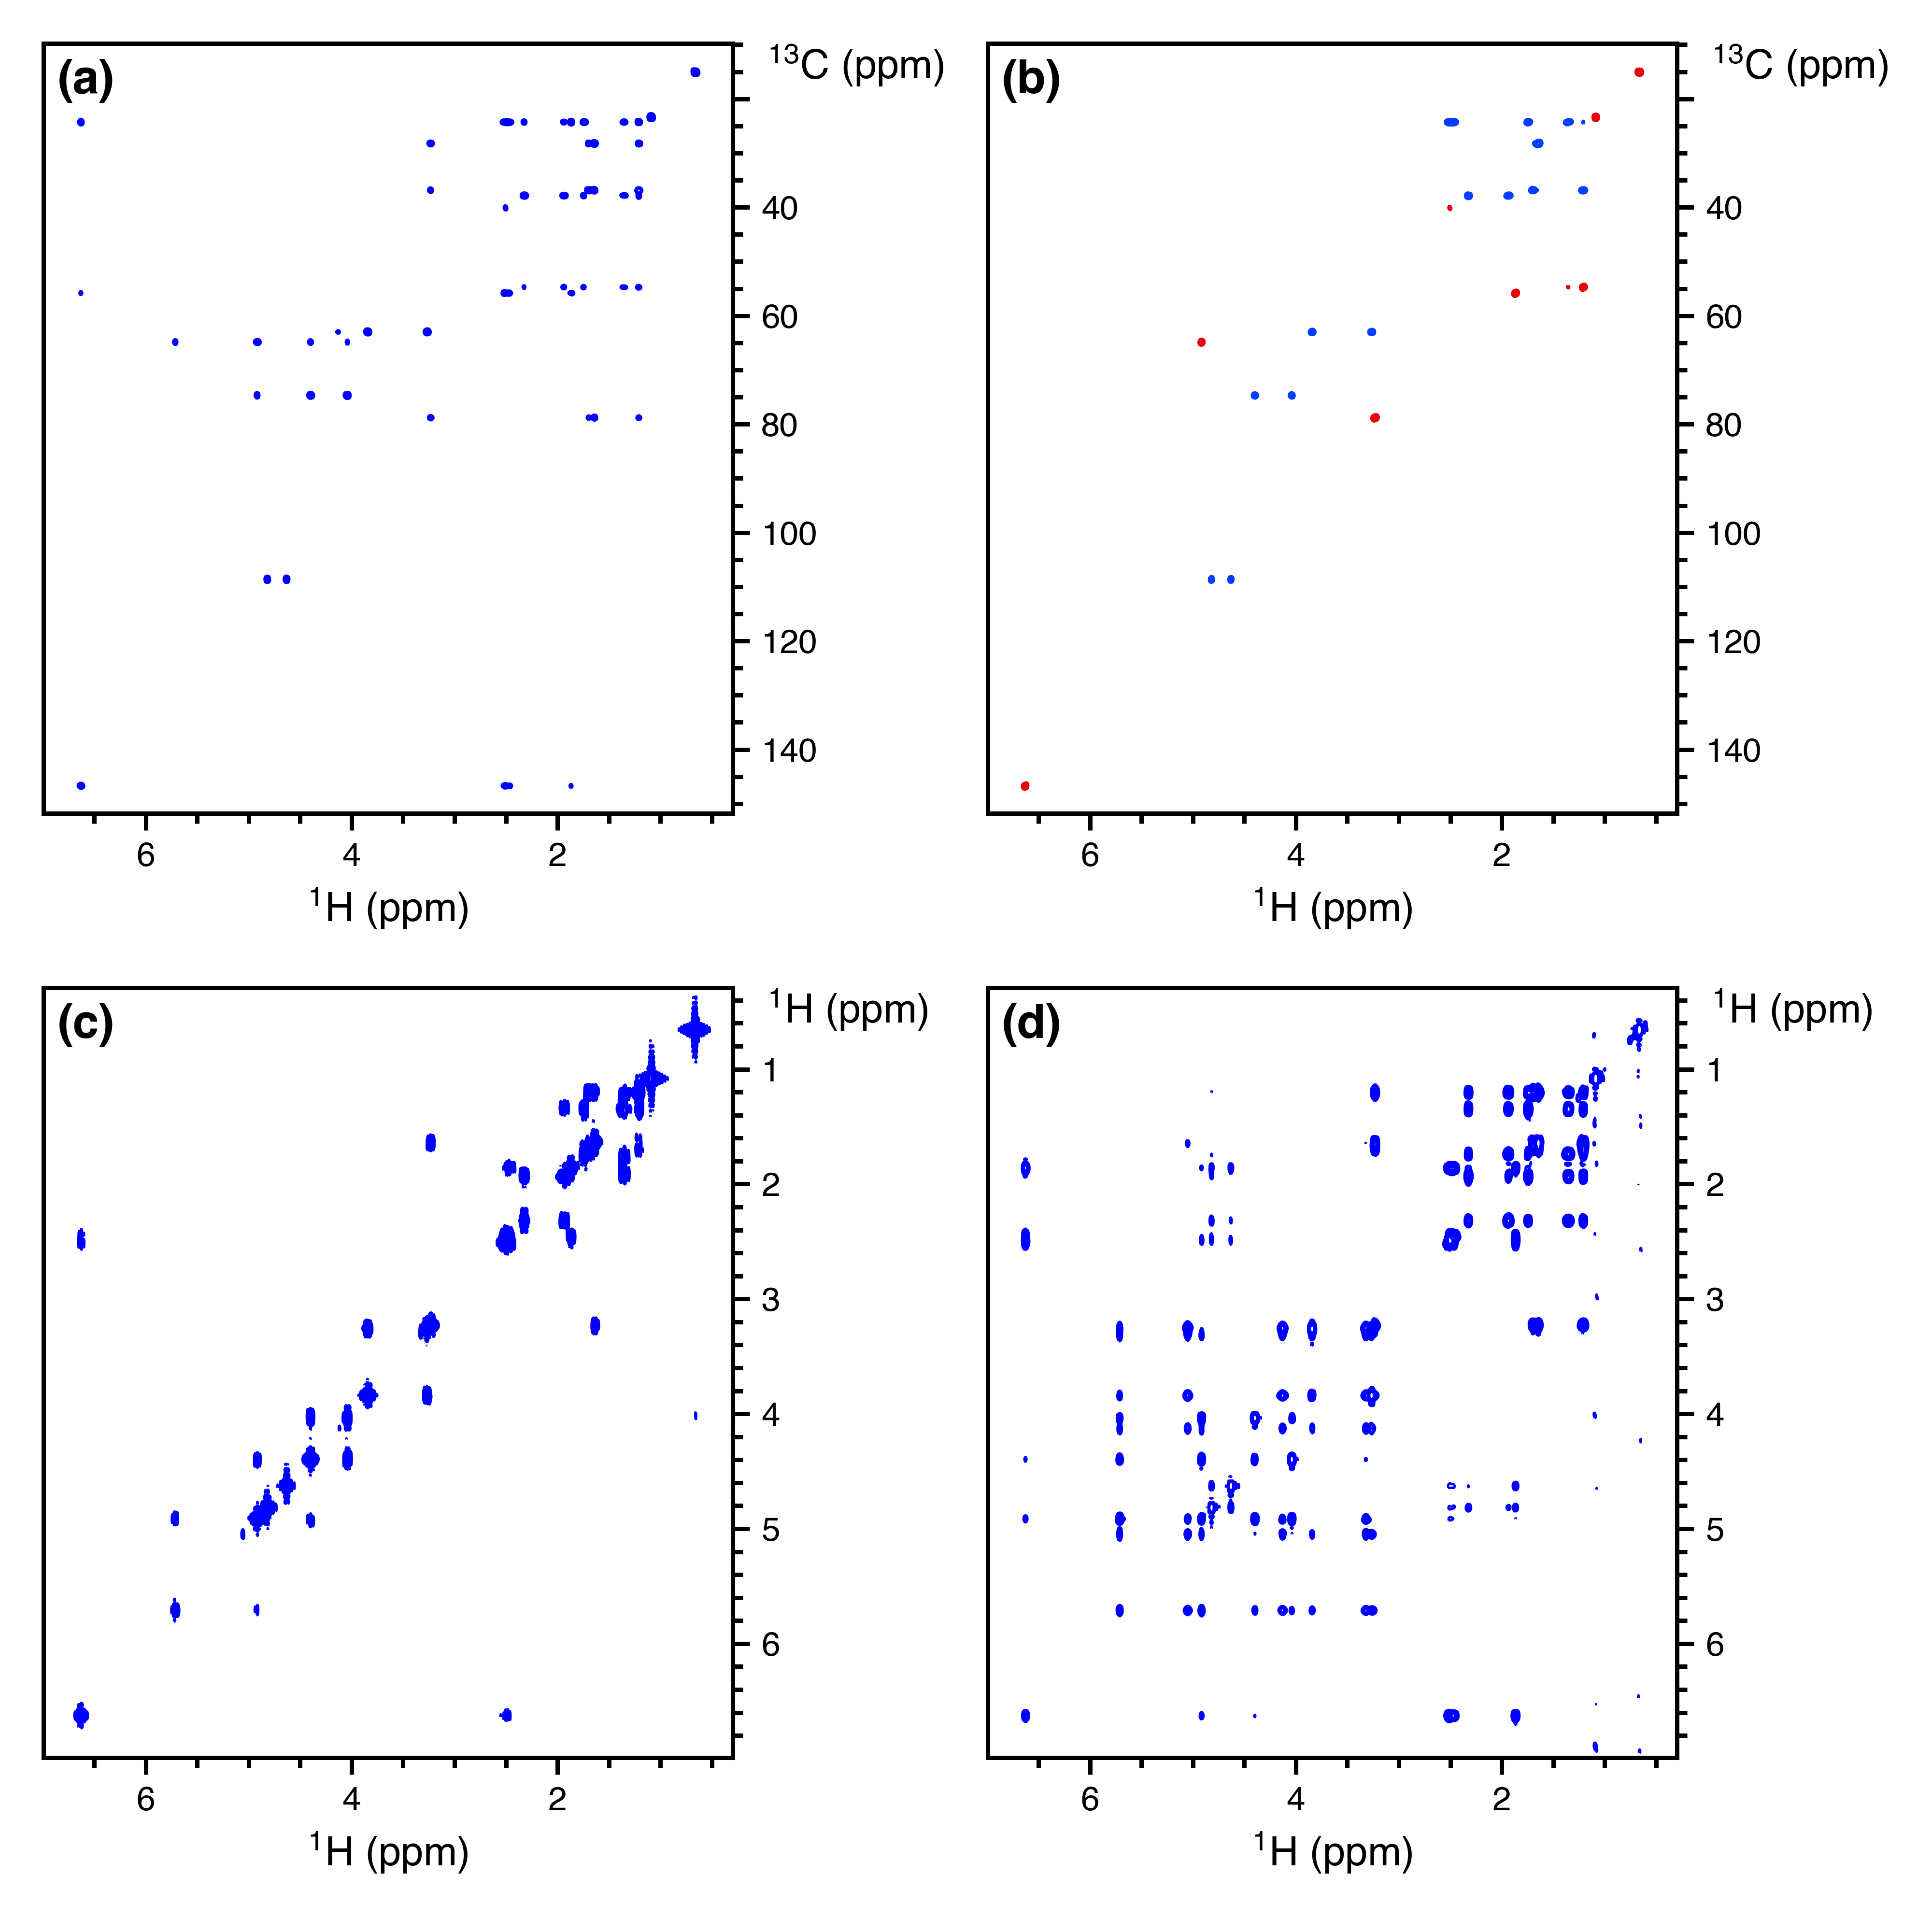
\includegraphics[width=0.8\textwidth]{stspct.png}
    \caption{
        2D spectra acquired using the NOAH-4 \noahfour{St}{Spb}{C}{T} supersequence.
        256 $t_1$ increments were used with 2 scans per increment, leading to a total experiment time of 17 minutes and 32 seconds.
        This represents a $3.25\times$ time saving relative to conventional acquisition of each of the four spectra with the same parameters, which would take a total of 57 minutes and 3 seconds.
        \textbf{(a)} HSQC-TOCSY (\SI{30}{ms} mixing time, $f = 0.9$).
        \textbf{(b)} Multiplicity edited seHSQC.
        \textbf{(c)} COSY.
        \textbf{(d)} TOCSY (\SI{60}{ms} mixing time).
        \andro{}
    }
    \label{fig:stspct}
\end{figure}

\begin{figure}
    \centering
    % figures/stspct_nus.py
    
\includegraphics{andro.png}\phantom{aaaaaa}
    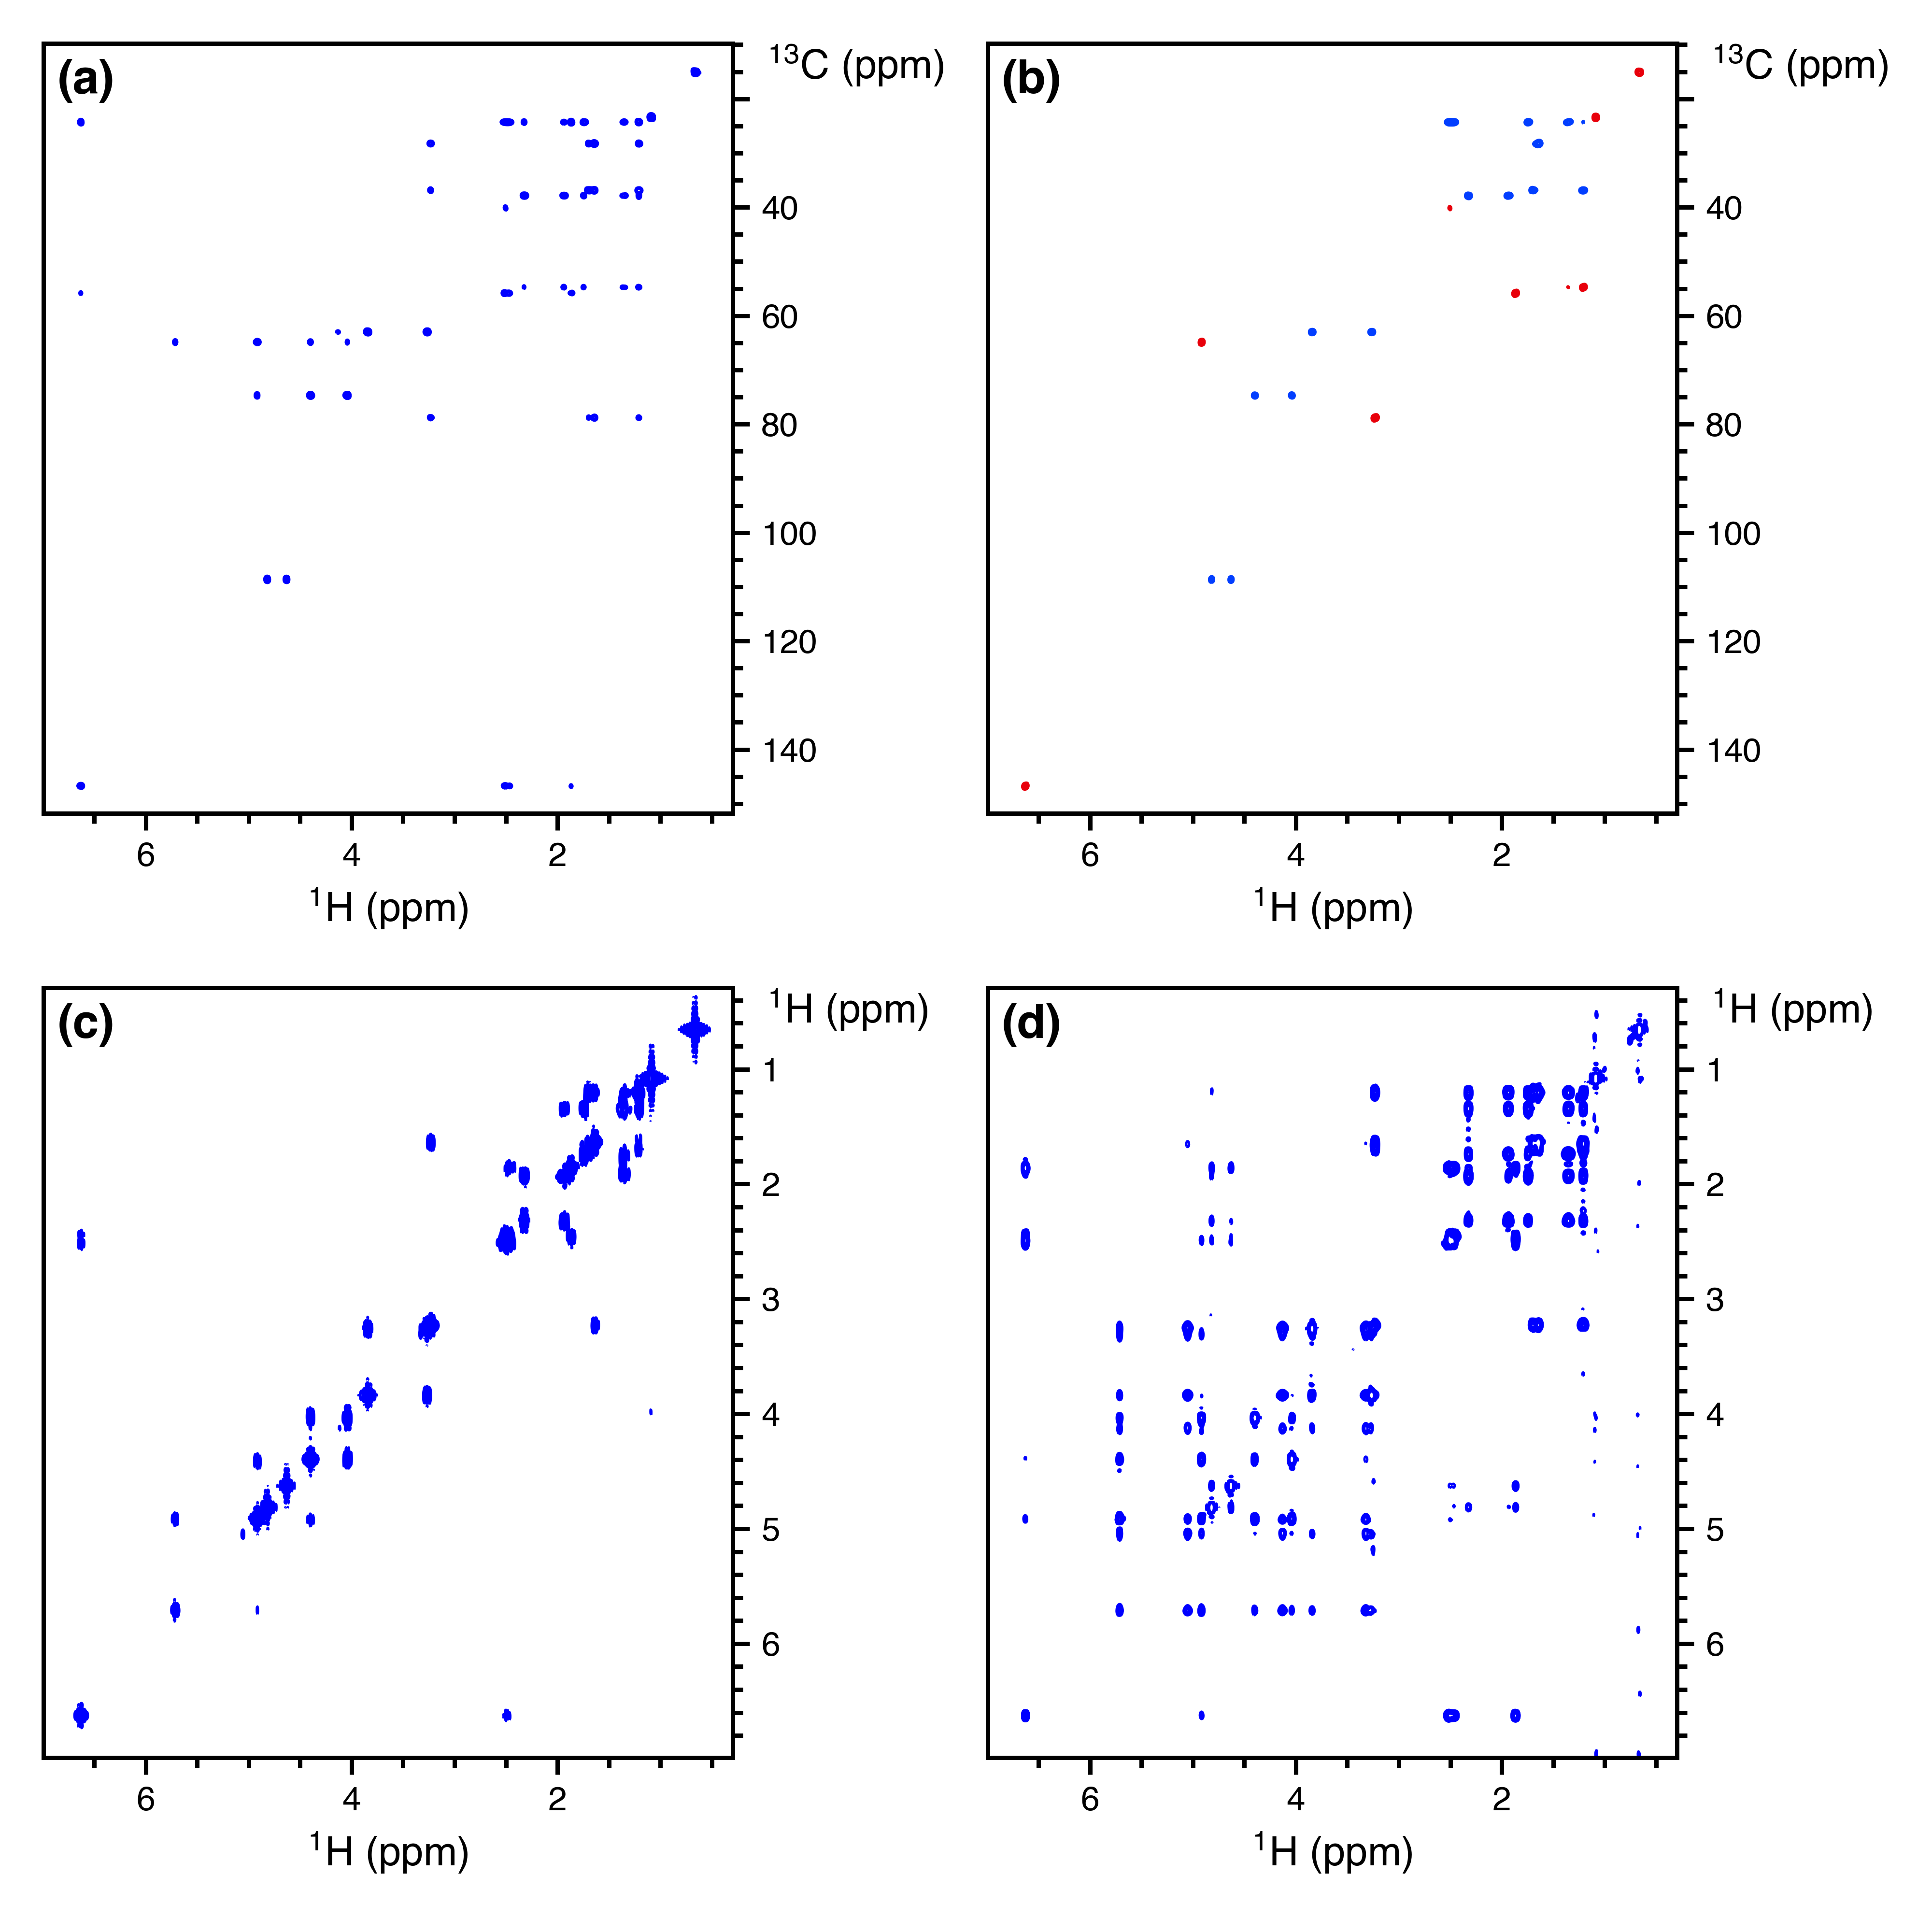
\includegraphics[width=0.8\textwidth]{stspct_nus.png}
    \caption{
        2D spectra acquired using the NOAH-4 \noahfour{St}{Spb}{C}{T} supersequence with 50\% non-uniform sampling for all modules.
        All other parameters are the same as in \cref{fig:stspct}.
        The experimental time was 9 minutes and 1 second.
        \textbf{(a)} HSQC-TOCSY (\SI{30}{ms} mixing time, $f = 0.9$).
        \textbf{(b)} Multiplicity edited seHSQC.
        \textbf{(c)} COSY.
        \textbf{(d)} TOCSY (\SI{60}{ms} mixing time).
        \andro{}
    }
    \label{fig:stspct_nus}
\end{figure}

\begin{figure}
    \centering
    % figures/bspnspcqf.py
    
\includegraphics{zolmi.png}\phantom{aaaaaa}

    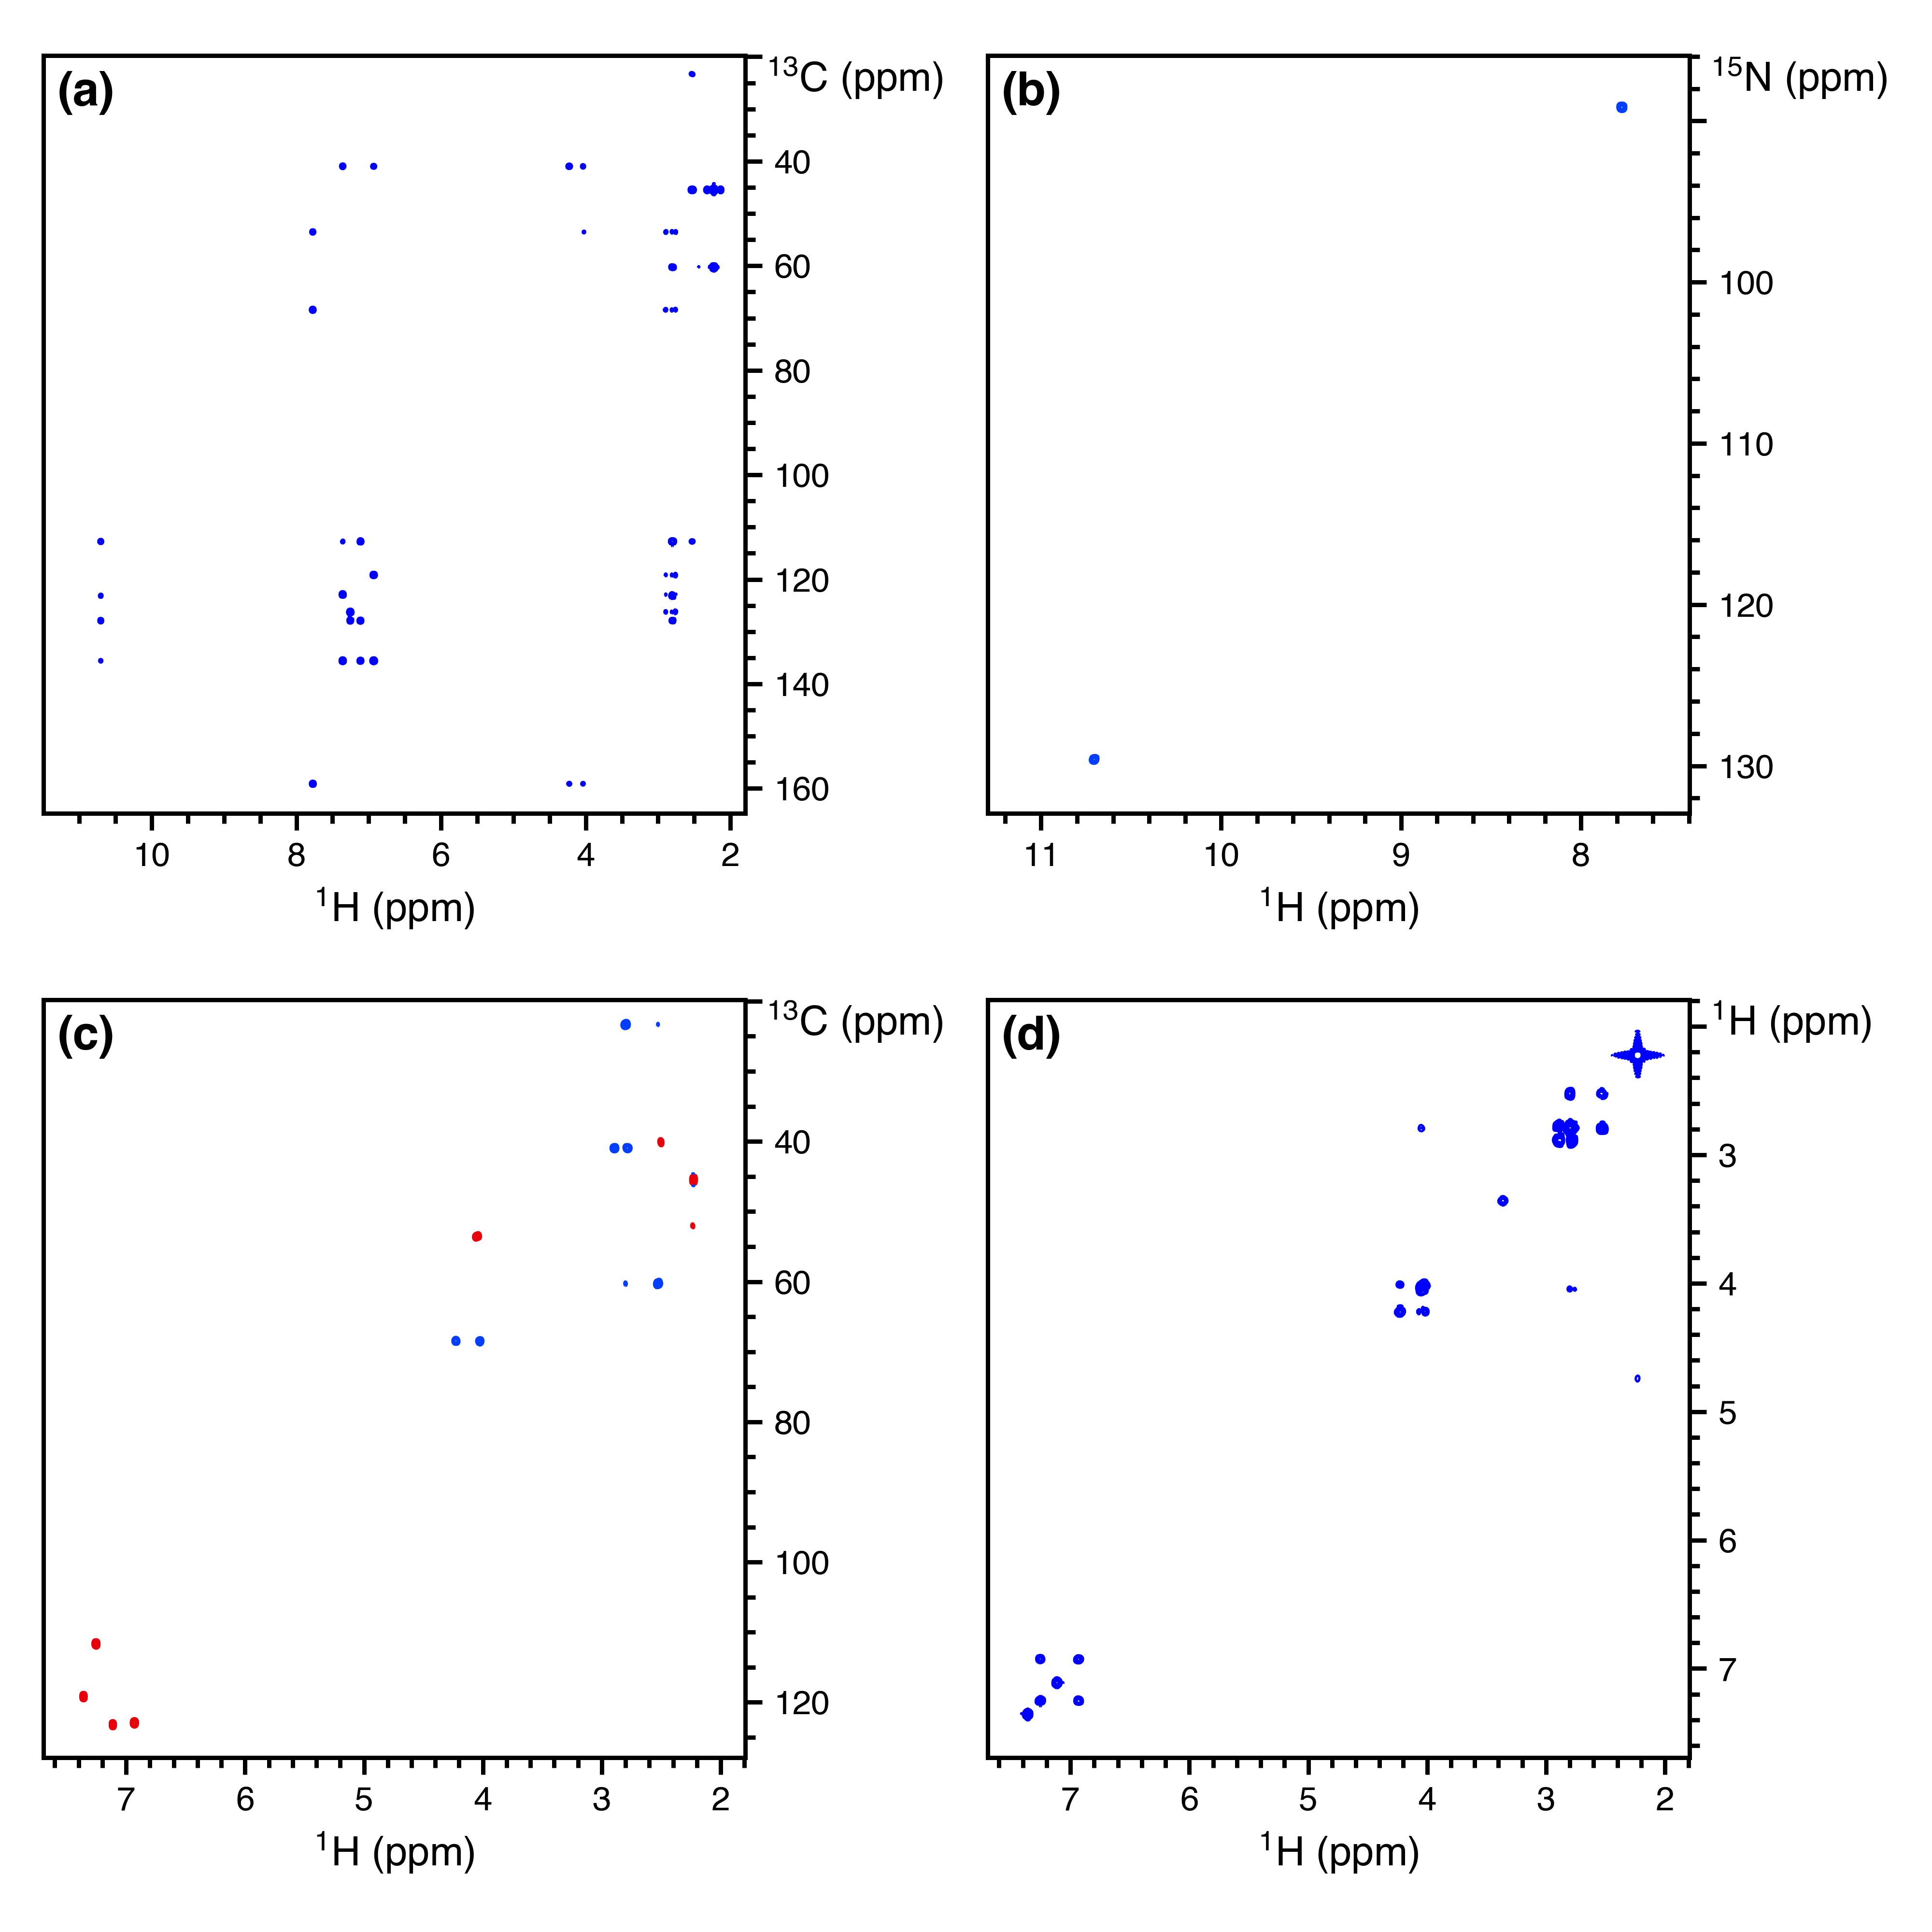
\includegraphics[width=0.8\textwidth]{bspnspcqf.png}
    \caption{
        2D spectra acquired using the NOAH-4 \noahfour{B}{Spn}{Spb}{Cqf} supersequence.
        256 $t_1$ increments were used with 2 scans per increment, leading to a total experiment time of 17 minutes and 32 seconds.
        This represents a $3.22\times$ time saving relative to conventional acquisition of each of the four spectra with the same parameters, which would take a total of 56 minutes and 28 seconds.
        \textbf{(a)} HMBC.
        \textbf{(b)} \nitrogen{} seHSQC with $k = 4$, linear predicted to 512 complex points.
        \textbf{(c)} Multiplicity edited \carbon{} seHSQC.
        \textbf{(d)} Magnitude-mode COSY (Bruker \texttt{qf} mode).
        \zolmi{}
    }
    \label{fig:bspnspcqf}
\end{figure}

\section{Sensitivity per unit time gains}

Whilst we have so far mainly focused on the \textit{time savings} that can be achieved via NOAH supersequences, it should also be noted that time savings can be translated into gains in sensitivity per unit time, according to the formula:\autocite{Kupce2019JMR,Kupce2021NRMP}

$$\varepsilon_t = R_S \cdot \sqrt{\rho_t}$$

where $\varepsilon_t$ is the relative sensitivity per unit time, $\rho_t$ is the time saving factor (i.e.\ the total experimental time needed for conventional acquisition, divided by the duration of the NOAH supersequence), and $R_S$ is a factor indicating the relative sensitivity of the NOAH module compared to a reference experiment.

$R_S$ may in general be less than 1 due to several factors:

\begin{enumerate}
    \item Imperfect retention of magnetisation by previous modules in a supersequence will reduce the value of $R_S$ for downstream modules.
        For example, the CLIP-COSY module in a \noahtwo{S}{Cc} or \noahtwo{Sp}{Cc} supersequence may have $R_S$ range from $\sim 0.1$ to $\sim 0.9$, depending on which variant of the (se)HSQC precedes it (\cref{tbl:sehsqc_comp_cosy}).
    \item Any modifications made to the sequence in order to achieve other aims such as artefact suppression or preservation of unused magnetisation components may lead to loss of signal.
        This is the case with, for example, the NOAH seHSQC modules, which have lower sensitivity compared to the original CRK implementation (\cref{fig:sehsqc_comp,fig:cnst16_diff}).
        It is also worth pointing out here that the \nitrogen{} seHSQC (\noahSpn{}) has a lower $R_S$ than the corresponding \carbon{} ZIP-seHSQC (\noahSpb{}), because of the extended CTP gradients present in the former (\cref{section:n15_cnst16_grads}).
\end{enumerate}

The value of $R_S$ for a given module therefore depends on each of the previous modules in a supersequence.
Since $R_S$ differs for each module in a supersequence, so does $\varepsilon_t$; if $\varepsilon_t > 1$ for a given module, then the supersequence can provide an increase in sensitivity per unit time for that module.

In \cref{fig:snr_modules} we demonstrated that $\varepsilon_t > 1$ for all four modules in the \noahfour{Spn}{Spb}{C}{T} supersequence.
The reference spectra there were taken to be the standalone NOAH modules, acquired as a set of four individual 2D experiments: thus, any reductions from $R_S$ must arise solely from item (1) above, as the sequences themselves are identical.

In \cref{fig:snr_bruker}, we perform the same comparison but this time using the ``gold standard'' 2D experiments (such as the CRK seHSQC) as the reference experiments: details of these experiments are provided in \cref{tbl:bruker_expts}.
This, together with the other SNR comparisons provided in this work, provide a measure of the losses in $R_S$ due to item (2) above.
Thus, the values of $\varepsilon_t$ are lower than in \cref{fig:snr_modules}.
However, we notably still have $\varepsilon_t > 1$ for the first three modules, and $\varepsilon_t \sim 1$ for the TOCSY, proving that NOAH supersequences do provide gains in sensitivity per unit time compared to conventional acquisition.

\begin{figure}
    \centering
    % figures/snr_bruker.py
    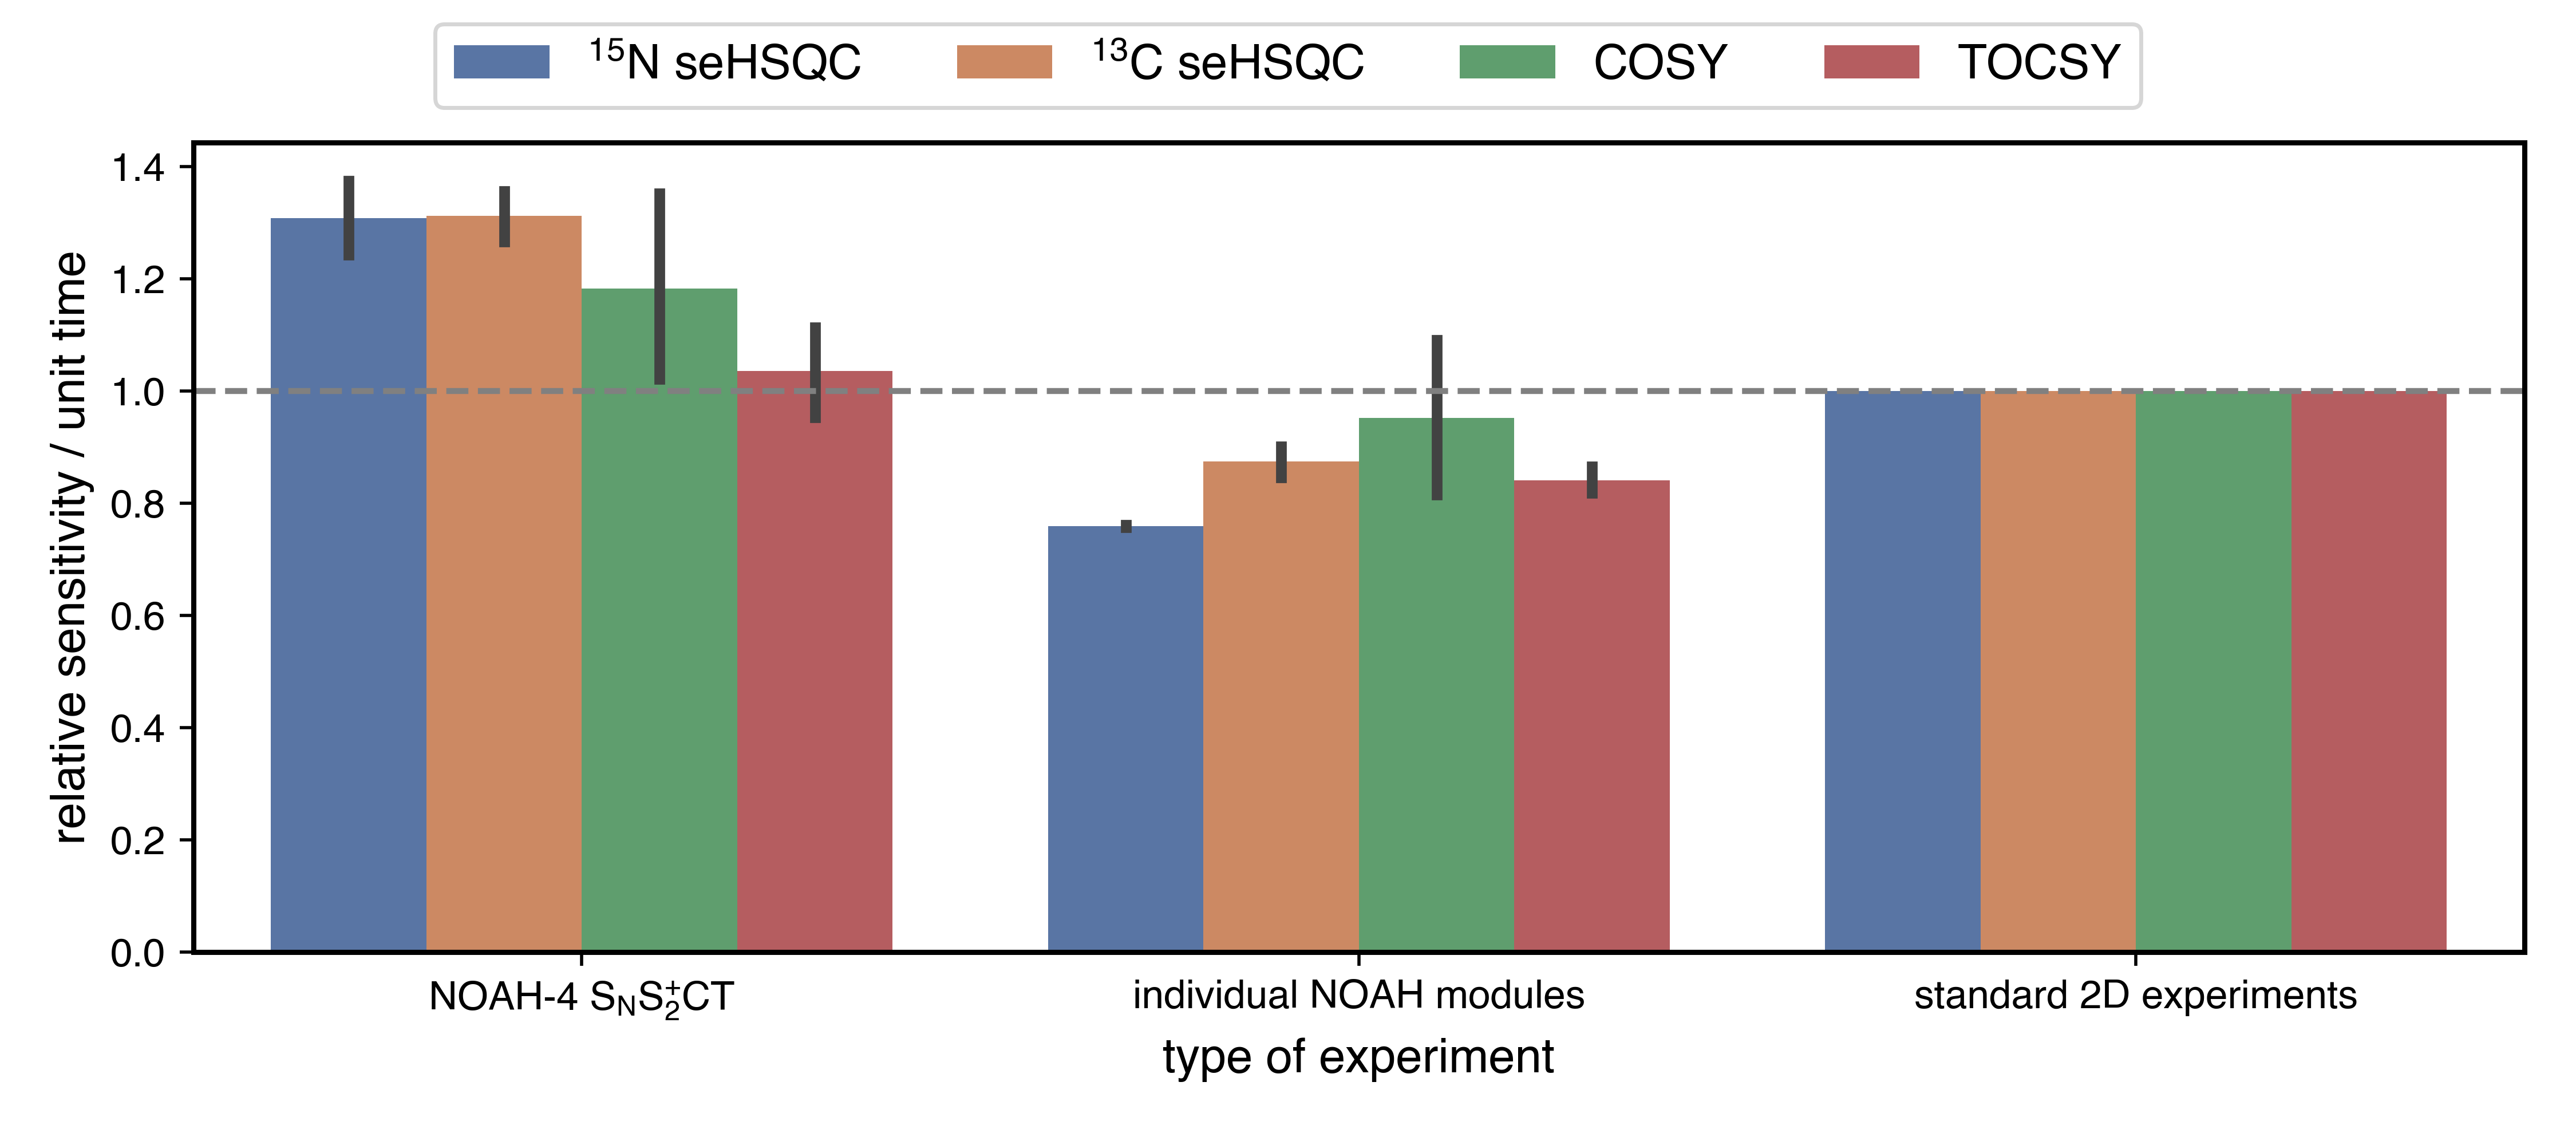
\includegraphics[width=0.9\textwidth]{snr_bruker.png}
    \caption{
        Relative sensitivities per unit time ($\varepsilon_t$) for the four modules in the \noahfour{Spn}{Spb}{C}{T} supersequence (using a TOCSY mixing time of \SI{35}{\ms}).
        Error bars indicate 95\% confidence intervals.
        Individually acquired standard 2D spectra were used as the reference spectra ($\rho_t = 3.24$).
        \zolmi{}
    }
    \label{fig:snr_bruker}
\end{figure}

{ % tbl:bruker_expts {{{2
\renewcommand{\arraystretch}{1.1}
\begin{table}
    \centering
    \begin{tabular}{cccccc}
        \toprule
        \textbf{Experiment} & \multicolumn{5}{c}{\textbf{Duration}} \\
                            & \nitrogen{} seHSQC & \carbon{} seHSQC & COSY & TOCSY & Total \\
        \midrule
        \textbf{NOAH-4}             & & & & & 17 min 28 s \\
        \midrule
        \textbf{Individual modules} & 14 min 36 s & 14 min 26 s & 14 min 13 s & 15 min 27 s & 58 min 42 s \\
        \midrule
        \textbf{Standard 2Ds}       & & & & & 56 min 35 s \\
        \texttt{hsqcetf3gpsi2}      & 14 min 5 s \\
        \texttt{hsqcedetgpsisp2.3}  & & 14 min 1 s \\
        \texttt{cosygpqf}           & & & 13 min 57 s \\
        \texttt{dipsi2gpphzs}       & & & & 14 min 32 s \\
        \bottomrule
    \end{tabular}
    \caption{
        Details of experiment times and pulse sequences used for comparisons of sensitivity per unit time (\cref{fig:snr_modules,fig:snr_bruker}).
        \zolmi{}
    }
    \label{tbl:bruker_expts}
\end{table}
} % }}}2

\printbibliography[heading=bibintoc,title={References}]
